\documentclass[12pt]{article}
\usepackage[a4paper]{geometry}
\usepackage[dvipsnames]{xcolor}
\usepackage{lipsum}
\usepackage{framed}
\usepackage{graphicx}
\usepackage[basque]{babel}
\usepackage{setspace}
\usepackage{indentfirst}
\usepackage{booktabs}  
\usepackage[table]{xcolor}
\usepackage{subcaption}
\usepackage[dvipsnames]{xcolor}
\usepackage{amsmath}
\usepackage{amssymb}
\usepackage{fontspec}
\usepackage{extpfeil}
\usepackage{siunitx}
\sisetup{output-decimal-marker = {,}}
\usepackage{wrapfig}
\usepackage{hyphenat}
\setlength{\parindent}{20pt}
\usepackage[style=phys, sorting=none, biblabel=brackets]{biblatex}
\addbibresource{tfgfisica.bib}
\usepackage{enumitem}
\usepackage{caption}
\setlength{\aboverulesep}{0pt}
\setlength{\belowrulesep}{0pt}
%%%%%%%%%%%% LETRAREN ITURRIA ALDATZEKO (EHUSerif) %%%%%%%%%%%%
\setmainfont{EHUSerif-Light.otf}[ % Nombre completo del archivo Regular
  Path = ./EHU Serif/,                        % Cambia esto si las fuentes están en una subcarpeta
  BoldFont = EHUSerif-Regular,     % Nombre completo del archivo Bold
  ItalicFont = EHUSerif-Italic, % Nombre completo del archivo Italic
  BoldItalicFont = EHUSerif-BoldItalic, % Nombre completo del archivo BoldItalic
]
\newfontface\lightfont{EHUSerif-Light.otf}[Path=./EHU Serif/]
\newfontface\blackfont{EHUSerif-Black.otf}[Path=./EHU Serif/]
\numberwithin{figure}{section}
\numberwithin{equation}{section}

\addto\captionsbasque{%
  \renewcommand{\figurename}{irudia}
}

\makeatletter
\renewcommand{\fnum@figure}{\textbf{\thefigure\ \figurename}}
\makeatother

\addto\captionsbasque{%
  \renewcommand{\tablename}{taula}
}
\makeatletter
\renewcommand{\fnum@table}{\textbf{\thetable.\ \tablename}}
\makeatother

\newcommand\blankpage{%
    \null
    \thispagestyle{empty}%
    \addtocounter{page}{-1}%
    \newpage}

\geometry{top=2.5cm, bottom=2.5cm, left=2.5cm, right=2.5cm}
\begin{document}
\setstretch{1.0}
\definecolor{light-gray}{gray}{0.87}  

\begin{titlepage}
\hspace*{-3.5cm}
    \begin{minipage}{\textwidth}
        \vspace{-2.5cm}
        \begin{center}
    

            
\includegraphics[width=\paperwidth]{LogoEHU.PNG}
        \end{center}
    \end{minipage}

\vspace{1cm}

\hspace{-3.5cm}
\noindent\fcolorbox {light-gray}{white}{

    \parbox{\paperwidth}{
     \begin{center}
     \large Gradu amaierako lana\\
     \large Fisikako gradua
     \end{center}
    }
    }


\vspace{0.8cm}

\noindent\hspace*{-2.5cm}%
\colorbox{light-gray}{\begin{minipage}{\paperwidth}%

    \vspace{1cm}

    \color{RoyalBlue}
    \centering\Large\textbf{Linac-7 azeleragailu linealerako \textit{Wien Filter}\\ 
    baten diseinua eta simulazioa}
    \\


    \vspace{8cm}\mbox{}
  \end{minipage}
}
\vspace{0.8cm}

\begin{flushright}
 Egilea:
\\
Urko Lopez Sacristan
\\
Zuzendariak:
\\
Iñigo Arredondo López de Guereñu
\\
Jorge Feuchtwanger Morales                  
\\
\end{flushright}

\vspace{1cm}

\hspace{-3.5cm}
\noindent\fcolorbox {light-gray}{white}{
    \begin{minipage}[]{1000pt}

        \parbox{\paperwidth}{
            \begin{center}
    
                 Leioa, 2025eko ekainaren 19a

            \end{center}
        }
    \end{minipage}
}
\end{titlepage}


%%%%%%%%%%%%%%%%%%%%%%%%%%%%%%%
%Hemendik aurrera hasi lana idazten%
%%%%%%%%%%%%%%%%%%%%%%%%%%%
\blankpage

\tableofcontents
\thispagestyle{empty}
\setcounter{page}{0}
\newpage

\section{Sarrera}
1927an, Ernest Rutherfordek laborategietan partikulak energia altuetara azeleratzeko beharra azpimarratu zuen, garaian desintegrazio erradioaktibo naturaletatik sortutako partikulak baino ez zirelako erabilgarriak \cite{rutherford_address_1997}. Horri erantzunez, eta soilik bost urte geroago, Cockroft eta Waltonek tentsio altuak lortzeko zirkuitu biderkatzaile bat diseinatu eta hidrogenotik sortutako protoiak 200 kV-etara azeleratzea lortu zuten \cite{cockcroft_experiments_1997}. \\

Ordutik, partikula azeleragailuen teknologia etengabe garatu da, izpien energiak keV-etatik TeV-etara igaroz, eta funtsezko tresnak bihurtu dira energia altuko fisikaren ikerkuntzan. Horren adibide esanguratsuena da 2012an LHC azeleragailuan Higgs bosoiaren existentziaren lehen froga esperimentala \cite{aad_observation_2012}. \\

Hala ere, horien erabilera ez dago oinarrizko fisikaren ikerkuntzara mugatuta. Areago, munduan existitzen diren 50000 partikula-azeleragailuetatik erdia industria aplikazioetan erabiltzen dira, ioi-ezarpenerako batez ere, eta gainontzeko handia berriz medikuntza aplikazioetan, radioterapian bereziki \cite{sheehy_applications_2024}. Aplikazio aniztasun handi honek etengabeko garapena eskatzen du, bi helburu nagusirekin: alde batetik, errendimendua eta kalitatea hobetzea; eta bestetik, eskuragarritasuna hobetzea, azeleragailu txikiago eta merkeagoak eraikiz.

\subsection{Linac-7 proiektua}
\label{sec:sarrera}
Premia horiek asetzeko, 2018an Euskal Herriko Unibertsitateko IZPILab Laborategiak Linac-7 proiektua azaleratu zuen, bertako hainbat industria-enpresen lankidetzarekin \cite{feuchtwanger_new_2022}. Proiektuaren helburua, izenak berak islatzen duen moduan, energia eta intentsitate baxuko protoi azeleragailu lineal bat diseinatzea eta eraikitzea da, ahalik eta trinkoena eta merkeena izanik. Horrez gain, Euskal Herrian partikula azeleragailuetan aditua den ikerketa-talde bat eratzea du helburu ere.\\

Linac-7-ren aplikazio nagusiena PET (\textit{Positron Emission Tomography}) diagnostikoarentzat beharrezkoak diren erradiofarmakoak produzitzea da \cite{victor_etxebarria_manufacturing_2022}. Gaur egun, aktibitate handiko eta erdibizitza luzeko erradioisotopo kaltegarriak erabiltzea ohikoa da, sortze-zentroetatik ospitaleetara garraiatu behar baitira. Ondorioz, proiektuaren kostu eta tamainaren funtsezko abantaila pazienteentzako berehalako dosiak lokalki sortzea da. Protoientzat aukeratutako 7 MeV-eko energiari esker, erdibizitza laburreko positroi-igorle ugari sor daitezke, hala nola $^{18}F$, $^{15}O$, $^{13}N$ eta $^{11}C$.\\

Esperotako energia lortzeko, azeleragailua sei etapaz osatzen da (1.1 Irudia):
\begin{enumerate}[itemsep=0em, topsep=0.8em]
    \item \textbf{\textit{Electron Cyclotron Resonance}} (ECR) ioi-iturria.
    \item \textbf{\textit{Low Energy Beam Transport}} (LEBT).
    \item \textbf{\textit{Radio Frequency Quadrupole}} (RFQ).
    \item \textbf{\textit{Medium Energy Beam Transport}} (MEBT).
    \item \textbf{\textit{Drift Tube Linac}} (DTL).
    \item \textbf{\textit{Beam Stop}}.
\end{enumerate}

\begin{figure}[h]
    \centering
    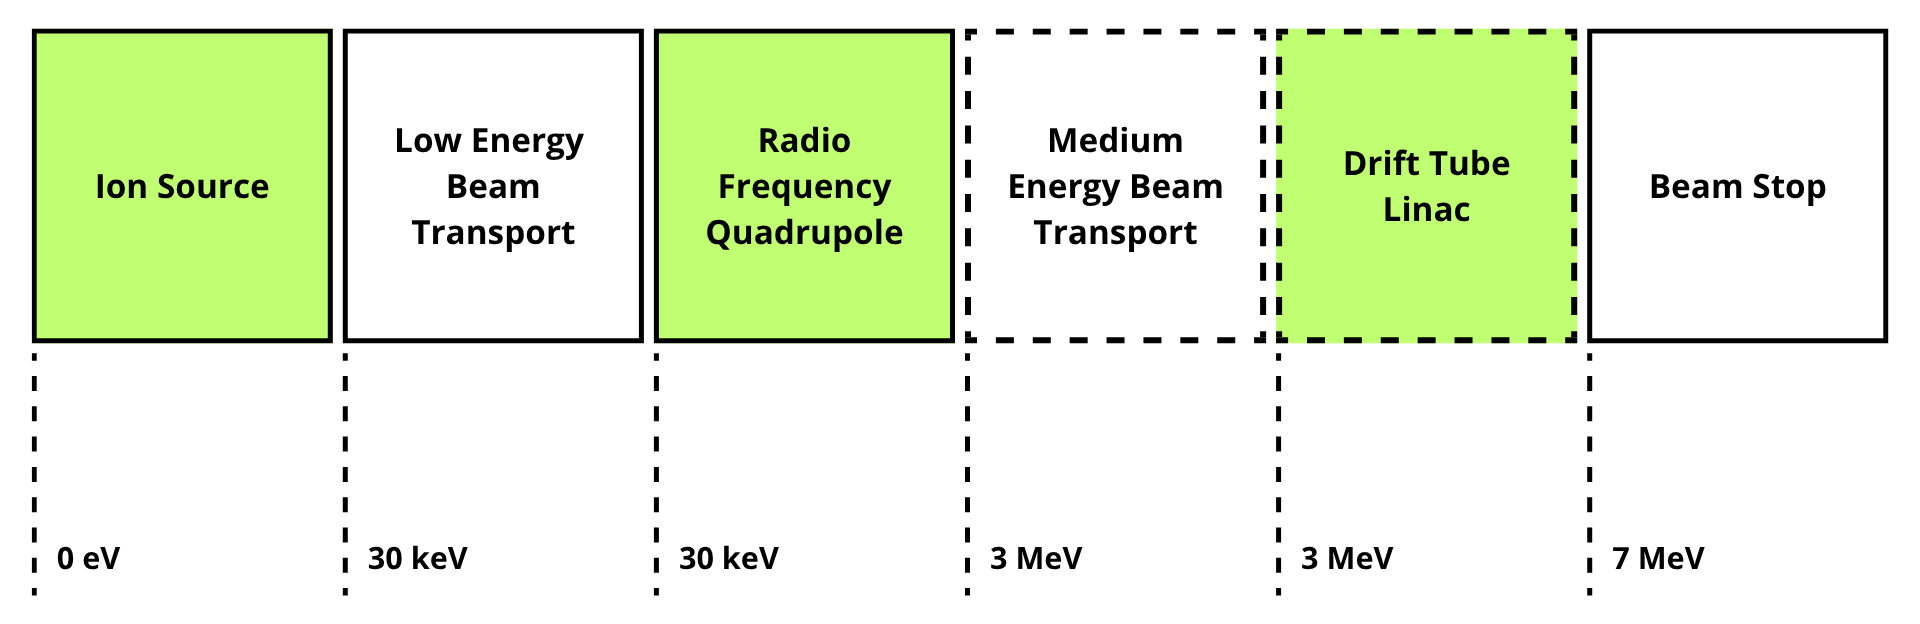
\includegraphics[width=\linewidth]{1 - Sarrera/etapas linac7.png}
    \caption{Linac-7 azeleragailuaren etapen eskema sinplea. Ertz eteneko etapak ez daude eraikita. Atzekaldea kolorezkoa dutenak azelerazio etapak dira.}
    \label{fig:linac7etapak}
\end{figure}
Lehenik eta behin, mikrouhinekin sortutako hidrogeno plasma batetik ioiak erauzten dira, 30 kV-eko elektrodo bat erabiliz. Ondoren, LEBT sistemak izpia solenoideen bidez egokitzen du RFQ-ra sartzeko egokia izan dadin, bertan 3 MeV-etaraino azeleratuko baita. MEBT-ak berriz ere izpia doitzen du hurrengo etapa azeleratzailera sartu baino lehen, bukaeran 7 MeV-eko energia lortuz, eta azkenik, izpia segurtasunez gelditzen da.\\

Lehenengo hiru etapak jada eraikita daude eta proba ugari aurrera eraman dira, baina MEBTa eta DTLa oraindik diseinu fasean daude. Testu honetan lehenengo bi etapetan soilik sakonduko da.

\subsection{ECR eta Plasma}
\label{sec:ecrplasma}

Edozein azeleragailuren lehen osagaia ioi-iturria da. Kasu honetan, PIT30 deituriko ioi-iturria erabiltzen da (\textit{Protoi Iturri Trinkoa 30 keV})\cite{elorza_romera_pit30_2021} elektroien ziklotroi-erresonantzia (ECR) erabiliz plasma ionizatzeko eta bertatik ioiak erauzteko (\ref{fig:pit30iturria}. irudia). \\

ECR ioi-iturrietan eremu magnetiko konstante bat ($\Vec{B}$) sortzen da plasma\hyp{}ganbaran, eta horren eraginpean, elektroi askeek Lorentzen indarra jasaten dute, eremu horri perpendikularra den ibilbide zirkular bat deskribatuz. Biraketa maiztasunari ziklotroi-maiztasuna ($f_{ce}$) deritzo,\\

\begin{equation}
    f_{ce} = \frac{eB}{2\pi m_{e}}
\label{eq:ziklotroi}
\end{equation}
\\
non $e$ eta $m_e$ elektroiaren karga eta masa diren, hurrenez hurren. Orduan, ganbarari eremu magnetikoaz gain kitzikapen elektromagnetiko bat transmitituz gero, kitzikapenaren maiztasuna ($f_{EM}$) ziklotroi-maiztasunarekin bat badator, ECR erresonantzia agertzen da: elektroiek energia handia irabazten dute. Beraz, plasma-ganbaran gas bat injektatuz gero, elektroiek atomo neutroak ionizatzen dituzte, karga positiboak eta negatiboak banatuz, eta plasma sortuz.

\newpage
PIT30-ren kasuan, erresonantzia 3 GHz-ko maiztasunean gertatzeko diseinatuta dago, ganbaran $TE_{111}$ modoa kitzikatuz. \eqref{eq:ziklotroi} ekuazioaren arabera, elektroiek maiztasun horretan biratzeko beharrezko eremu magnetikoaren intentsitatea $B=110mT$ ingurukoa izan behar da.

\begin{figure}[h]
    \centering
    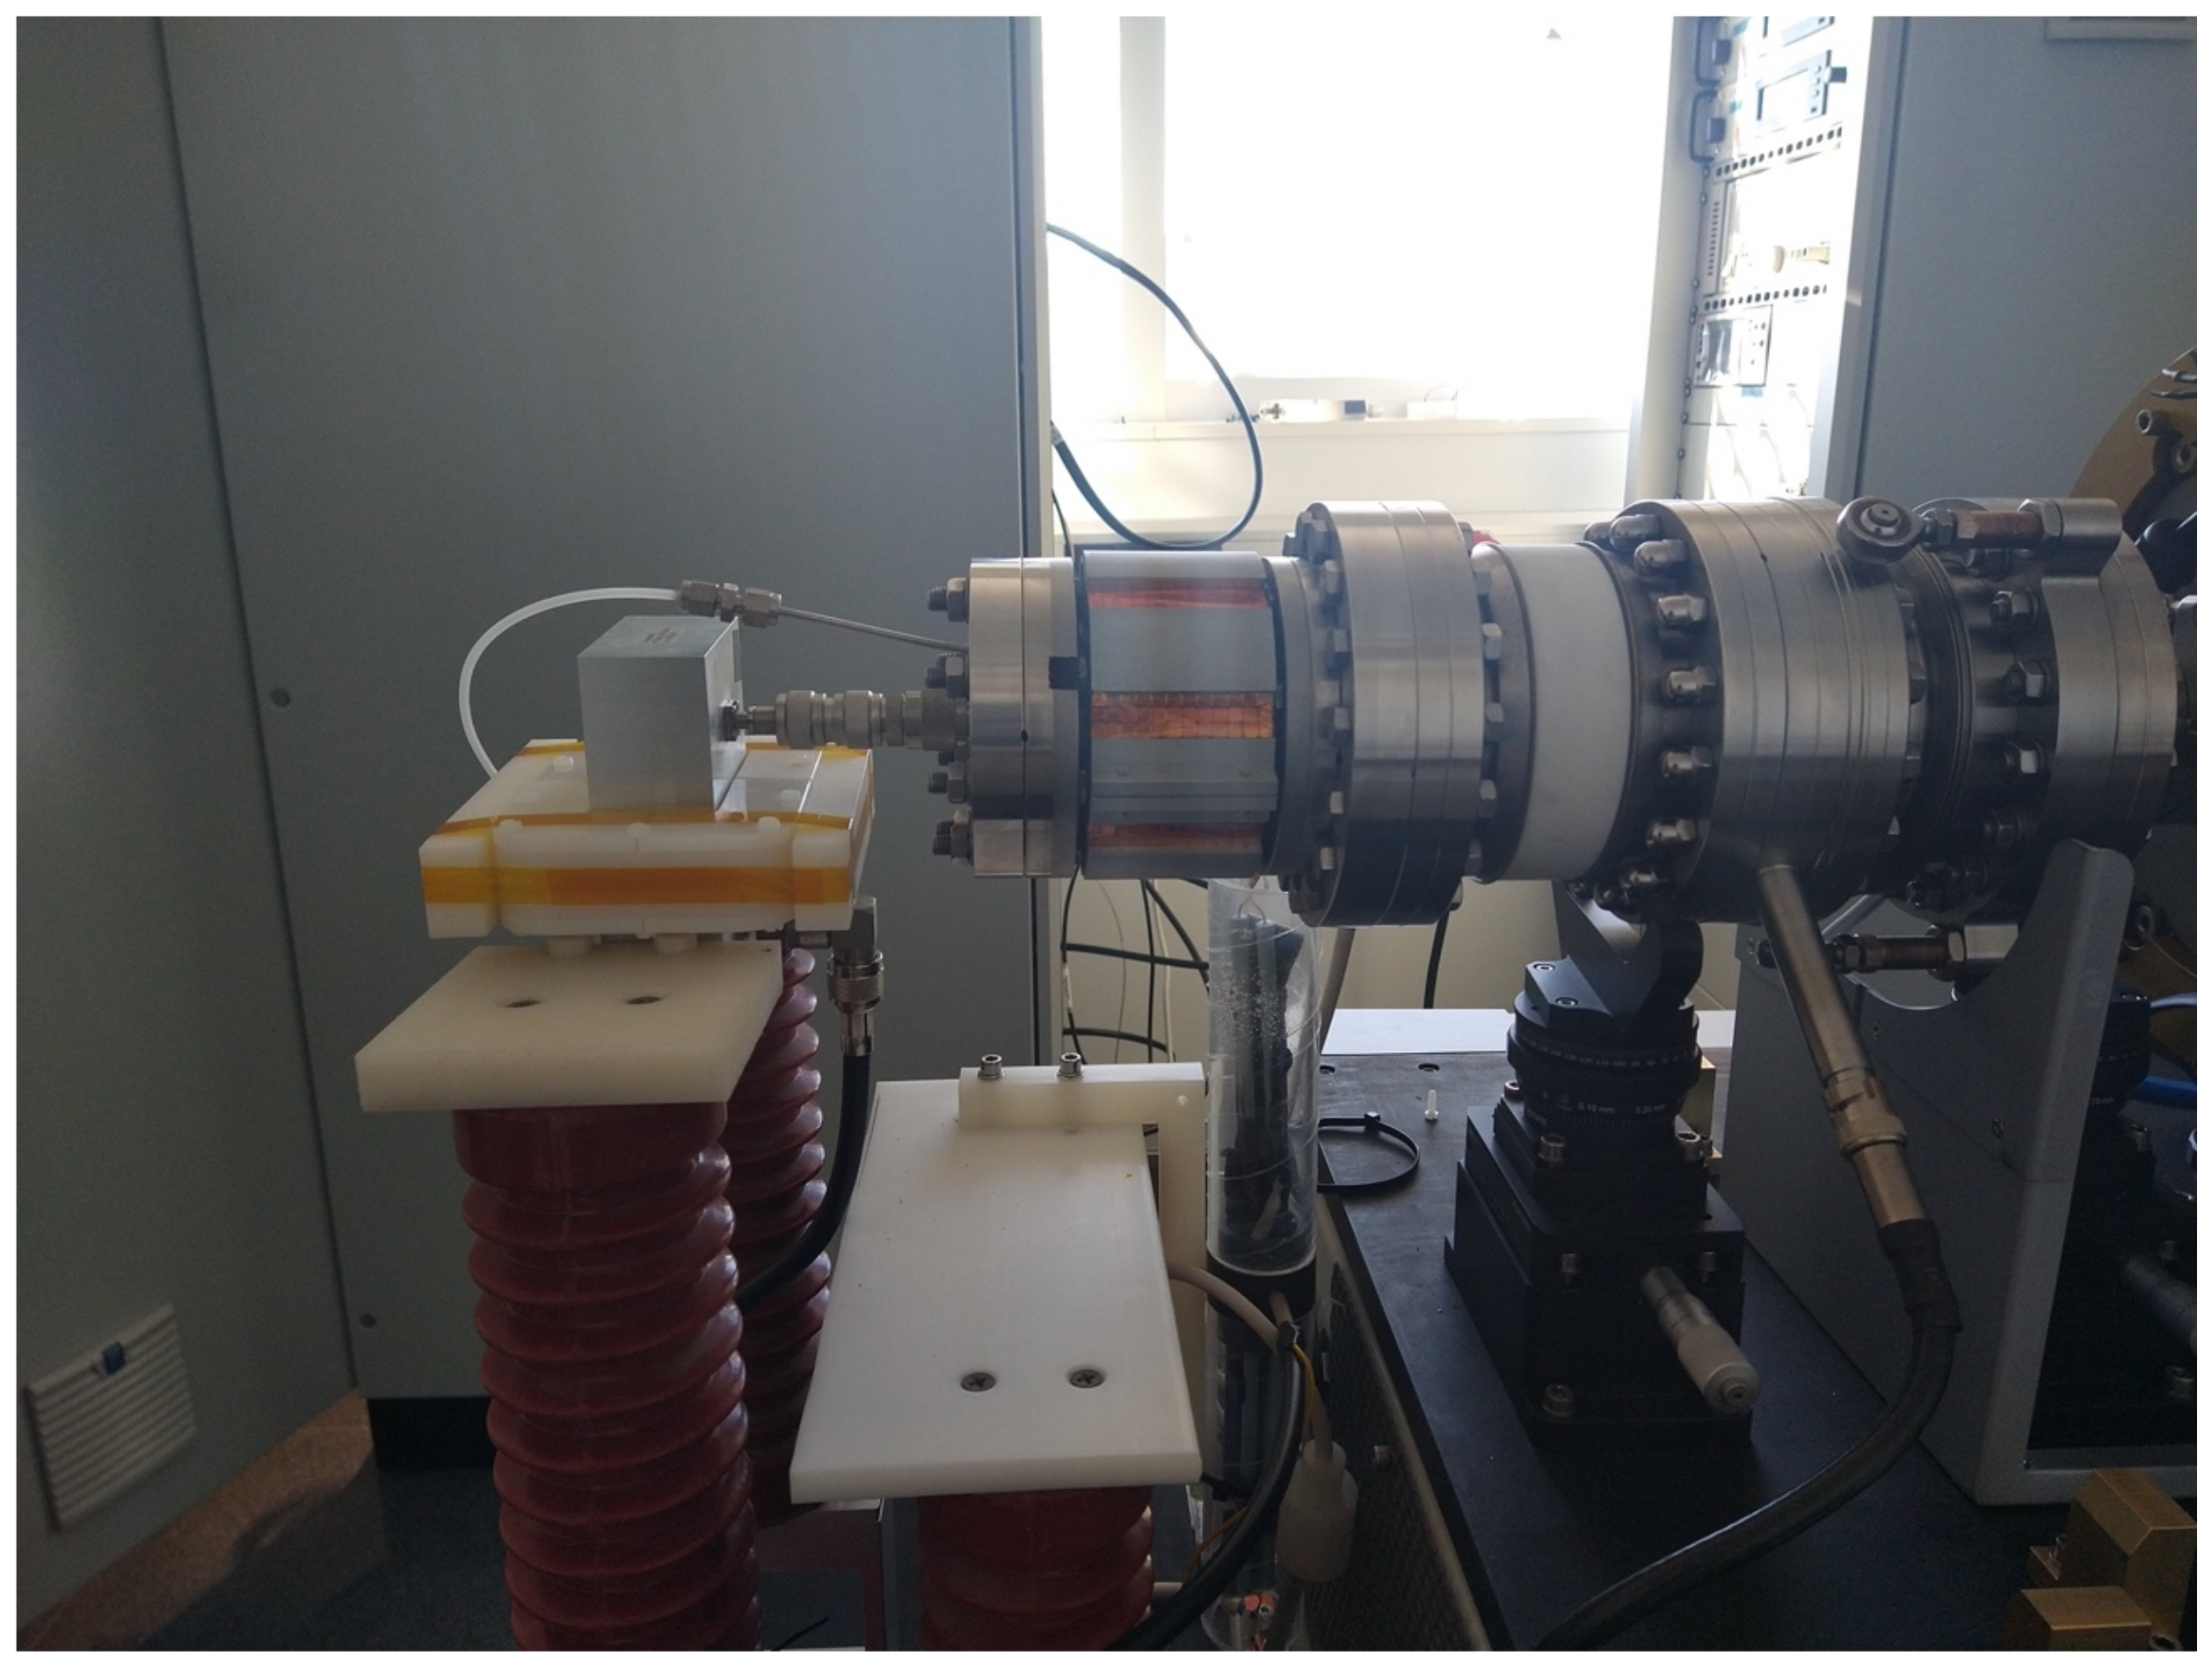
\includegraphics[width=0.5\linewidth]{1 - Sarrera/pit30argazkia.png}
    \caption{PIT30 ioi-iturriaren argazkia \cite{feuchtwanger_new_2022}.}
    \label{fig:pit30iturria}
\end{figure}

Iturri honetan plasma sortzeko erabiltzen den gasa hidrogenoa da, $H_2$, eta plasmaren erreakzioetan protoiak ($H^+$) sortzen dira. Beste hidrogeno espezie batzuk ere sortzen dira ($H_2^+$, $H_3^+$, $H$), eta ikusi da ganbarara transmititutako RF potentziaren arabera eta gas-fluxuaren arabera espezie batzuen sorkuntza beste espezieen aurrean gailentzen dela \cite{elorza_romera_modelo_2022}.

\begin{figure}[h]
    \centering
    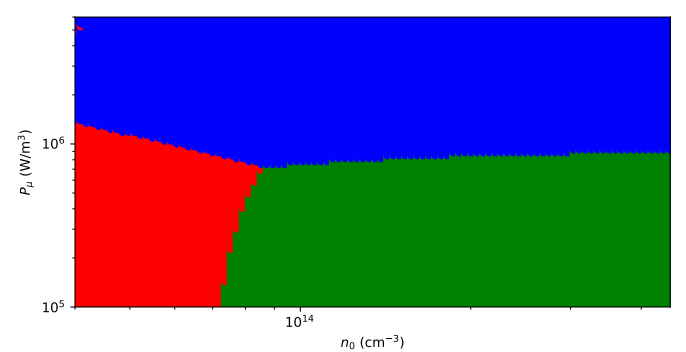
\includegraphics[width=0.8\linewidth]{1 - Sarrera/predominant_map.PNG}
    \caption{Espezie bakoitza (\colorbox{cyan}{$\mathbf{H_{ }^+}$}, \colorbox{red}{$\mathbf{H_2^+}$}, \colorbox{green}{$\mathbf{H_3^+}$}) gailentzen den zonaldeen mapa, potentzia-dentsitatearen eta gas-dentsitatearen arabera.}
    \label{fig:mapa}
\end{figure}
Azeleragailuaren hurrengo etapak protoientzat baino ez daudenez diseinatuta, garrantzitsua da protoi sorkuntza maximizatzea, parametro operazional zuzenak aukeratuz. Horrez gain, garrantzitsua da espezie desberdinen dentsitateak ezagutzea, eta posible bada, erabilgarriak ez diren espezieak iragaztea.
\newpage
\subsection{Espezieen hautaketa}

Hainbat teknika desberdin erabili daitezke espezie ionikoak hautatzeko. Lehendabizi, aipatzekoa da RFQ-ak iragazki modura jokatzen duela ere, oszilazio\hyp{}{}maiztasunekin bat ez datozen partikulak jatorriz baztertzen direlako, hurrengo etapetara sartzea saihestuz. Hala ere, ez da iragazki aktiboa, eta komenigarriagoa da diagnostiko arduratsuagoa egitea.\\

Iman hautatzaileek, adibidez, espezieak masa/karga ($m/q$) erlazioaren arabera desbideratzea ahalbidetzen dute; izan ere, kasu honetan iturrian sortutako ioiek karga berdina dutenez ($+q$) eta potentzial berdinarekin erauzten direnez ($\Delta V$), energia zinetiko berdina dute ($E_k = q \Delta V$), baina abiadura ($v$) desberdina masaren arabera. Orduan, imanek sortutako eremu magnetiko perpendikularretik ($B$) igarotzean, ibilbide zirkular desberdinak deskribatuko dituzte, ziklotroi erradioaren ($r_c$) arabera:\\

\begin{equation}
\left.
\begin{aligned}
    v &= \sqrt{\frac{2q \Delta V}{m}}\\\\
    r_c &= \frac{mv}{qB}
\end{aligned}
\right\}
\xRightarrow \\
r_c = \sqrt{\frac{m}{q}\frac{2 \Delta V}{B^2}}
\label{eq:hautatzaile}
\end{equation} \\

Horrela, imanen ondoren pantaila analizatzaile bat ipiniz gero, posiblea da espezieen bereizmena ikustea, eta talkek sortutako argitasunaren arabera baita espezieen dentsitateak lortzea ere (\ref{fig:hautatzaile}. irudia).\\

\begin{figure}[h]
    \centering
    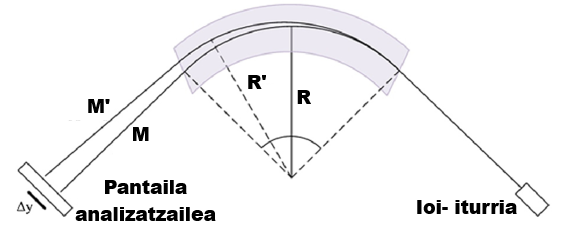
\includegraphics[width=0.5\linewidth]{1 - Sarrera/analizatzaile.png}
    \caption{90º-ko iman hautatzaile baten eskema sinplea \cite{lopes_mass_2011}.}
    \label{fig:hautatzaile}
\end{figure}

Hala ere, askotan partikulak ibilbidea kurbatu gabe banatzea beharrezkoa da, eta horretarako, \textit{Wien Filter} deituriko dispositiboak erabiltzen dira (\ref{fig:wienfilter}. irudia). Karga berdineko partikulak beren abiaduraren arabera bereizteko aukera ematen dute, eremu elektrostatiko ($E$) eta magnetostatiko ($B$) perpendikularrak baliatuz, lerro zuzenean. Eremuen konfigurazio horri esker, partikulek jasandako indar elektriko ($F_e$) eta indar magnetikoek ($F_m$) aurkako noranzkoa dute, eta  magnitudeak zuzen aukeratuz partikulen abiadura ($v_f$) hautatu daiteke,

\begin{equation}
\left.
\begin{aligned}
    F_e &= qE\\\\
    F_m &= qv_fB
\end{aligned}
\right\}
\xRightarrow \
\sum F = F_e - F_m = q (E - v_f  B) = 0\ \xRightarrow \ \boxed{ v_f = \frac{E}{B}}
\label{eq:hautatzaile}
\end{equation}

\begin{figure}[h]
    \centering
    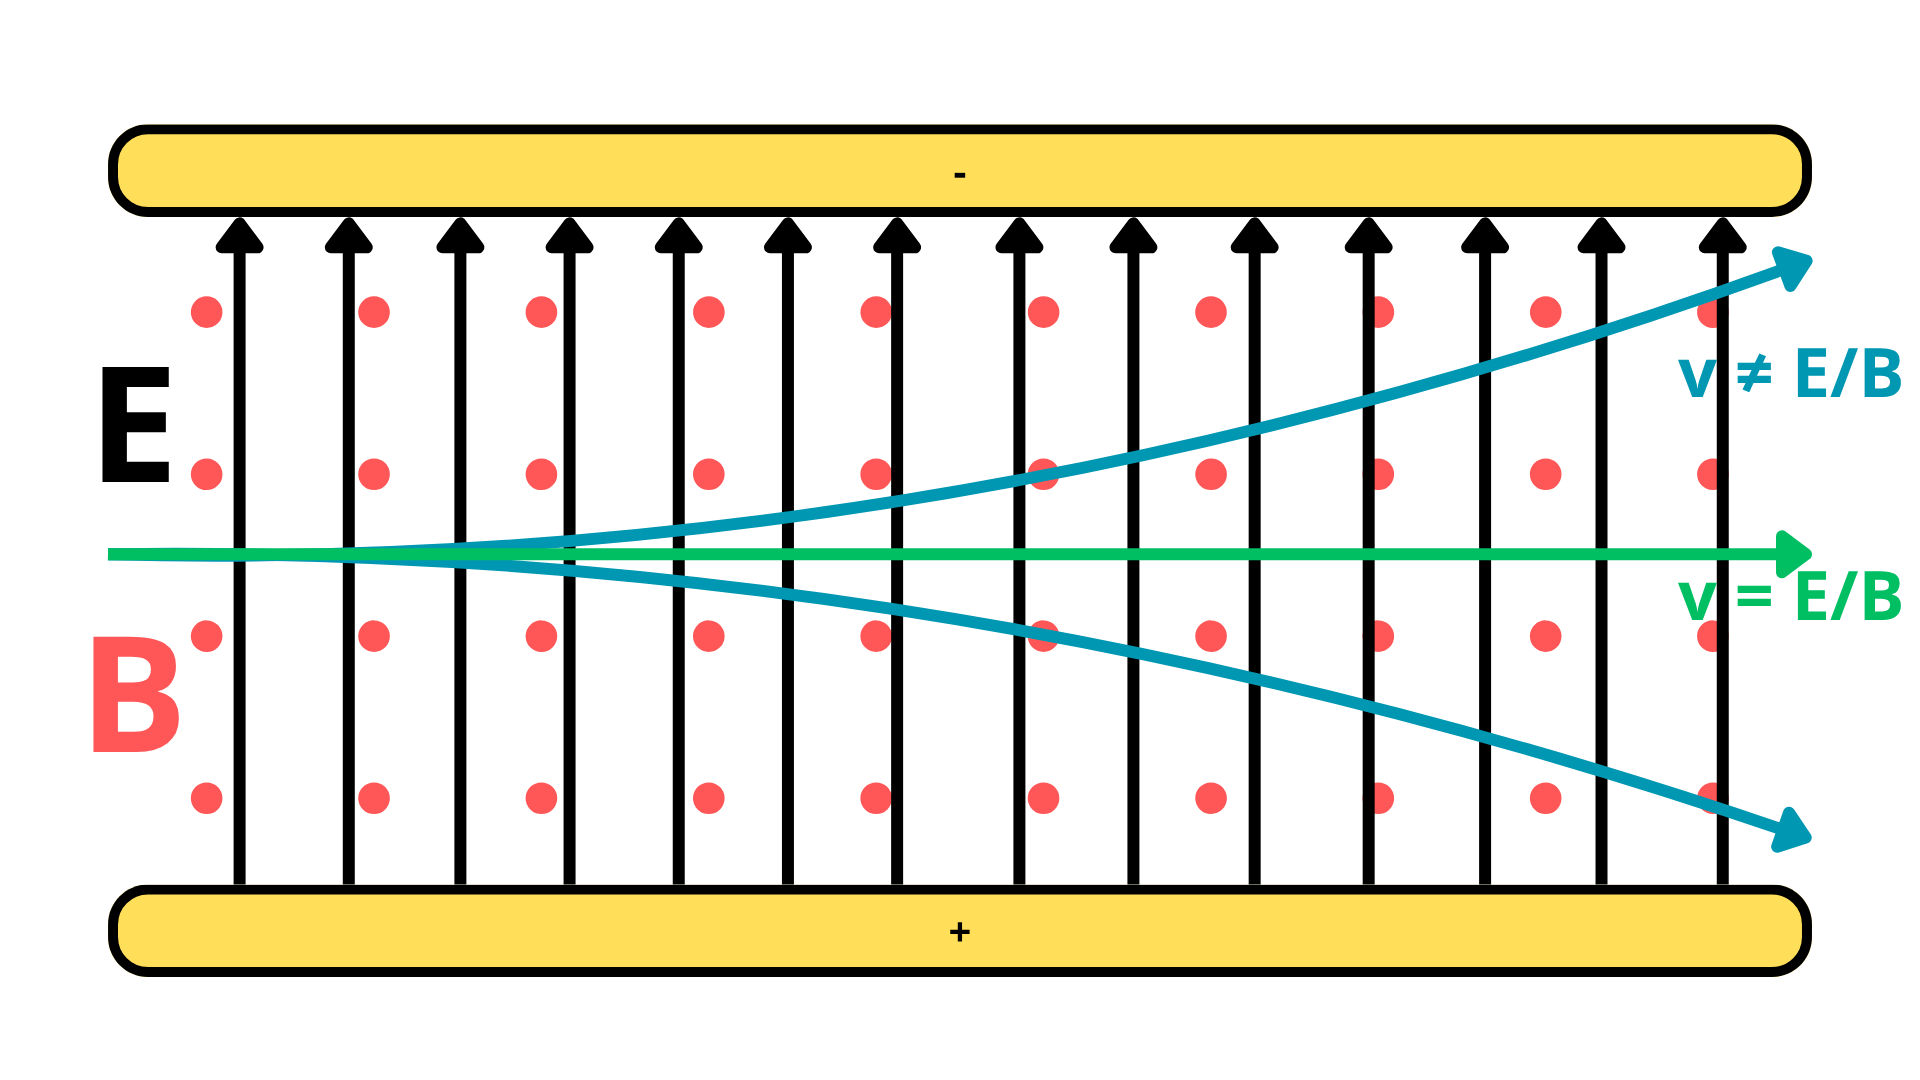
\includegraphics[width=0.5\linewidth]{1 - Sarrera/wienfilter.png}
    \caption{\textit{Wien Filter} baten eskema sinplea.}
    \label{fig:wienfilter}
\end{figure}

Aurreko guztia kontuan hartuta, eta LEBT-an sartzen diren espezieen abiadura erauzte\hyp{}potentzialak guztiz definitzen duenez, Linac-7 proiektuarentzako \textit{Wien Filter} bat diseinatzea erabaki da. Horrela, garapen prozesuan espezie desberdinak aukeratu daitezke, dentsitateak ezagutzeko eta plasmaren diagnostiko zuzen bat gauzatzeko \textit{Faraday cup}-a erabiliz (\ref{fig:faradaycup}. irudia). Areago, amaierako muntaian ere erabilgarria izango da, RFQ-ra protoiak baino ez direla sartzen ziurtatzeko.

\begin{figure}[h]
    \centering
    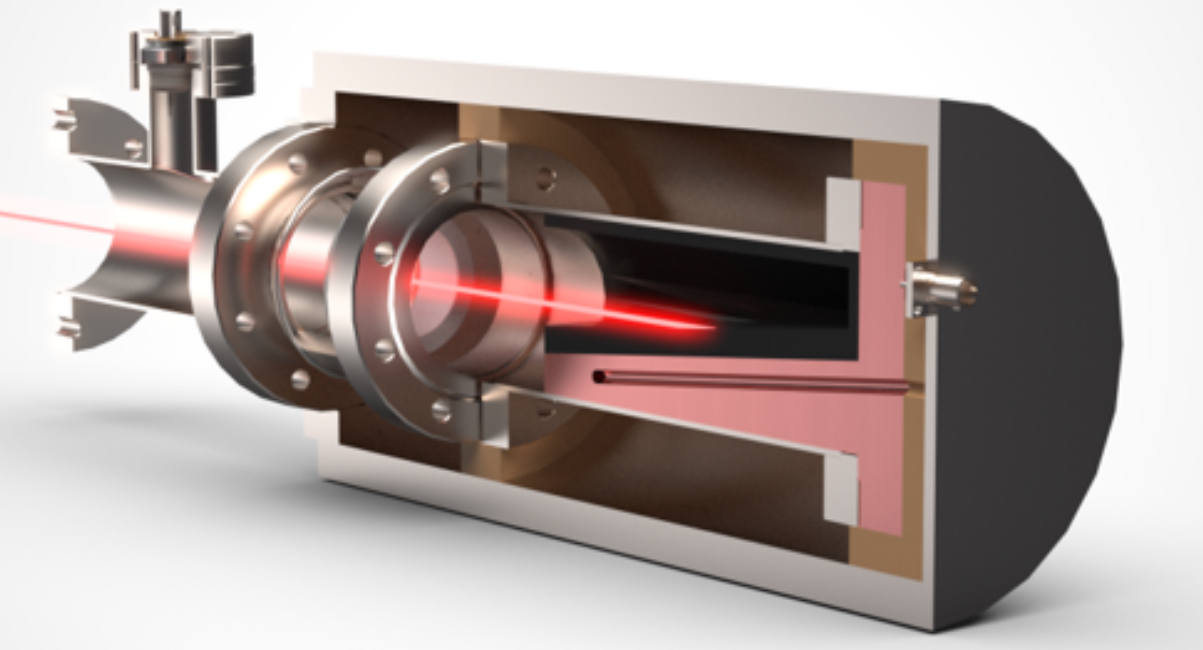
\includegraphics[width=0.45\linewidth]{1 - Sarrera/faradaycup.png}
    \caption{Linac-7 azeleragailuaren azken etapa, \textit{Faraday cup}-a (\textit{Beam Stop}) \cite{feuchtwanger_new_2022}.}
    \label{fig:faradaycup}
\end{figure}

\subsection{Helburuak}

Testu honen helburu nagusia Linac-7 proiektuarentzako \textit{Wien Filter}-aren lehen diseinu bat garatzea eta simulatzea da.\\

Hala ere, helburu hori lortzeko, garrantzitsua da lehenik dispositibora sartuko den izpia ondo ezaugarritzea, eta horretarako ezinbestekoa da plasman eta erauzte-sisteman sakontzea. Aurretik garatutako hidrogeno plasmaren modelizazio bat aurkeztu eta erabiliko da \cite{elorza_romera_modelo_2022} simulatuko diren espezieen dentsitate frakzioak zehazteko, eta izpia ulertzeko beharrezkoak diren propietateak azalduko dira. \\

Horrez gain, simulazioak gauzatzeko COMSOL Multiphysics softwarea \cite{noauthor_comsol_2025} erabiliko da, nahiz eta proiektuan orain arte SIMION softwarea \cite{noauthor_simion_2020} erabili den partikulen ibilbidea simulatzeko. Ondorioz, COMSOL-en trebatzea funtsezkoa da, eta baita aurretik egindako simulazioekin emaitzak balidatzea.\\

Azkenik, \textit{Wien Filter}-aren eremu elektriko eta magnetikoen ertz-efektuetan sakonduko da simulazioen bidez, idealtasun teorikoen mugak aztertuz, ahalik eta diseinurik errealena eta eraginkorrena gauzatzeko.



\newpage
\section{Oinarri teorikoa}
\subsection{Hidrogeno plasma}
\label{sec:plasma}
Helburuen atalean aipatu den moduan, ioi-iturrian sortzen den plasma hobeto ulertzeko, eta erauzketaren simulazioetan ahalik eta izpirik errealena lortzeko, Mikel Elorzak garatutako hidrogeno-plasmarako modelo globala erabiliko da \cite{elorza_romera_modelo_2022}.\\

Modelo honek plasman sortzen diren espezie guztien dentsitateentzako soluzio geldikor bat kalkulatzea ahalbidetzen du. Horretarako, hurrengo ekuazio\hyp{}sistema ez-lineala iteratiboki ebazten da, zentzuzko soluzio konbergente bat lortu arte:


\begin{align}
    n_{H^+} + n_{H_2^+} + n_{H_3^+} - n_e &= 0 \label{eq:neutraltasuna}\\
    \sum_{i} R_{sorrera,s,i} - \sum_{i} R_{galera,s,i} &= 0 \label{eq:partikulaoreka}\\
    \frac{P_{plasma}}{V_{plasma}}-e\sum_{j}n_1 n_2 k_j \epsilon_{c,j} - \sum_{X}u_{B,X} n_X \frac{A_{eff}}{V}(\epsilon_i + \epsilon_e) &= 0 \label{eq:termodinamikaoreka}
\end{align}

\eqref{eq:neutraltasuna} ekuazioa neutraltasun baldintza da. Plasma ioi-kargadunen multzoa izan arren, mikrometroak baino eskala handiagotan neutrotzat hartu daiteke, ioien arteko apantailamenduaren ondorioz. Beraz, positiboki eta negatiboki kargatutako espezieen dentsitateak ($n_{H^+},\;n_{H_2^+},\;n_{H_3^+},\;n_e$) orekan egon behar dira.\\

\eqref{eq:partikulaoreka} adierazpenak, ordea, bost ekuazio desberdin ematen ditu, espezie bakoitzerako ($s$) bat. Espezie bakoitzaren aldaketa-tasen orekak deskribatzen dituzte; hau da, plasman gertatzen diren erreakzio guztiak jakinik (\ref{fig:plasmaerreakzioak}. irudia), soluzio geldikorrean espezieen sorrera ($R_{sorrera,i}$) eta galera ($R_{galera,i} $) orekan egon behar da. Erreakzio-tasak honela definitzen dira,

\begin{equation}
\begin{aligned}
    R = k \prod_j n_j \qquad k = \langle \sigma v \rangle_E
\end{aligned}
\label{eq:erreakziotasa}
\end{equation}
\\
non $n_j$ erreaktiboen dentsitateak diren eta $k$ erreakzio-koefizientea den, sekzio-eraginkorraren ($\sigma$) eta partikulen abiaduraren ($v$) biderkadura gisa adierazten dena. Dena den, partikula guztiek abiadura berdina ez dutenez, energia-banaketa Maxwelldarraren gaineko batezbestekoa kalkulatzen da.\\

Azkenik, \eqref{eq:termodinamikaoreka} ekuazioan energia oreka deskribatzen da, ganbarara transmititutako mikrouhinetik plasmak xurgatzen duen potentziaren arabera ($P_{plasma}$):

\begin{itemize}
    \item Ezkerreko batukariak erreakzioetako talka elastiko eta inelastikoen bidez galtzen den energia adierazten du, $k_j$ sekzio-eraginkorraren, $n_{1,2}$ erreaktiboen dentsitateen eta $\epsilon_{c,j}$ galdutako batezbesteko energiaren funtzio. 
    \item Eskuineko batukariak ganbararen hormetan galtzen diren ioien energia zinetikoa adierazten du, $u_{B,X}$ Bohm-en abiaduraren, $n_X$ galdutako espezieen dentsitatearen, $A_{eff} = h_l 2\pi R^2$ galeren azalera efektiboaren, eta $\epsilon_i$ ioiek eta $\epsilon_e$ elektroiek galdutako batezbesteko energiaren funtzio.
\end{itemize}

\begin{figure} [h]
    \centering
    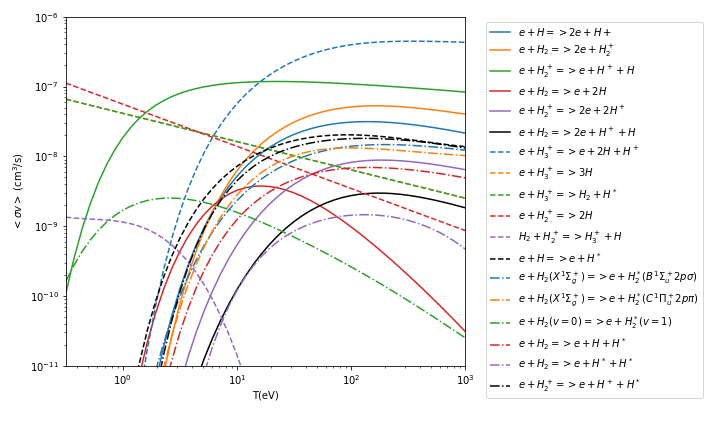
\includegraphics[width=0.9\linewidth]{2 - Oinarri teorikoa/hidrogeno erreakzioak.png}
    \caption{Elektroien eta hidrogeno espezieen arteko erreakzioak eta beren erreakzio-koefizienteak, elektroien-teneperaturaren funtzio \cite{elorza_romera_modelo_2022}.}
    \label{fig:plasmaerreakzioak}
\end{figure}

Beraz, zazpi ekuazio eta zazpi ezezagun \{$n_e,n_H,n_{H^+},n_{H_2^+}, n_{H_3^+}, T_e$\} izanik, ekuazio-sistema ebatz daiteke. $T_e$ elektroien tenperatura da, eta presio baxuko plasmetan $T_e \sim 1-10eV$ tartekoa izaten da.\\

Hainbat parametro definitzea beharrezkoa da ere: $R=\num{3.1}\;cm$ eta $L=10\;cm$ plasmaren luzera eta erradioa, $A_{eff}$ azalera efektiboaren kalkulurako beharrezkoak; $T_i=\num{0.2}\;eV$ eta $T_g=500\;K$ ioi positiboen eta gas-neutroaren tenperatura, erreakzio-koefizienteen kalkulurako beharrezkoak; eta azkenik, $\gamma=\num{0.1}$, ganbararen hormaren materialaren eta hidrogenoaren arteko errekonbinazio probabilitatea.\\

Horrez gain, PIT30-ren kasuan, ganbarara transmititutako RF potentzia eta gas-fluxua nahi bezala aldatu daitezke, baina ekuazioetan agertzen diren aldagaiak ($n_{H_2},P_\mu$) ez dira zuzenean tresnetan sartutakoak ($P_{aurrera}$ [W], $Q_{gas}$ [sccm]). Horiek lortzeko, datu esperimentaletan oinarritutako adierazpenak erabili dira,
\begin{align}
    P_\mu &= \frac{P_{plasma}}{V_{ganbara}} = \frac{(\alpha - \alpha_0)P_{aurrera}}{f\pi R^2L} \label{eq:potdentsitate} \\
    n_{H_2} &= \frac{n_{crit}}{Q_{crit}}Q \label{eq:gasfluxu}
\end{align}
\begin{itemize}
    \item Potentzia-dentsitatean ($P_{\mu}$), $(\alpha - \alpha_0)=\num{0.5}$ faktorea erabiltzen da xurgatutako ($\alpha)$ eta bero moduan xahututako ($\alpha_0$) potentzia diferentzia lortzeko. Bestalde, plasmak hartzen duen bolumena ganbararen osoa ez denez, $f=\frac{V_{plasma}}{V_{ganbara}}=\num{0.5}$ faktorea sartu behar da. 
    \item Gas-neutroaren dentsitatean ($n_{H_2}$), plasma pizteko beharrezko gas-fluxu minimoa ($Q_{crit}=\num{0.5}\;sccm$) erabiltzen da. Gainera, ereduan soluzioa existitzeko gas-neutro dentsitate minimo bat dagoela ikusi da ere ($n_{crit}=\num{2.2}\cdot 10^{13}cm^{-3}$).
\end{itemize}

Beraz, parametroak, ekuazioak eta aldagaiak izanik, espezieen dentsitateak lortu ditzakegu. Simulazioak sinplifikatzeko, soluzio bakarra bilatuko da, aldagaiak finkatuz. \ref{sec:ecrplasma} atalan aipatu den moduan, jakina da RF potentziaren eta gas\hyp{}fluxuaren arabera espezie batzuen sorkuntza gailentzen dela.

\begin{figure}[h]
    \centering
    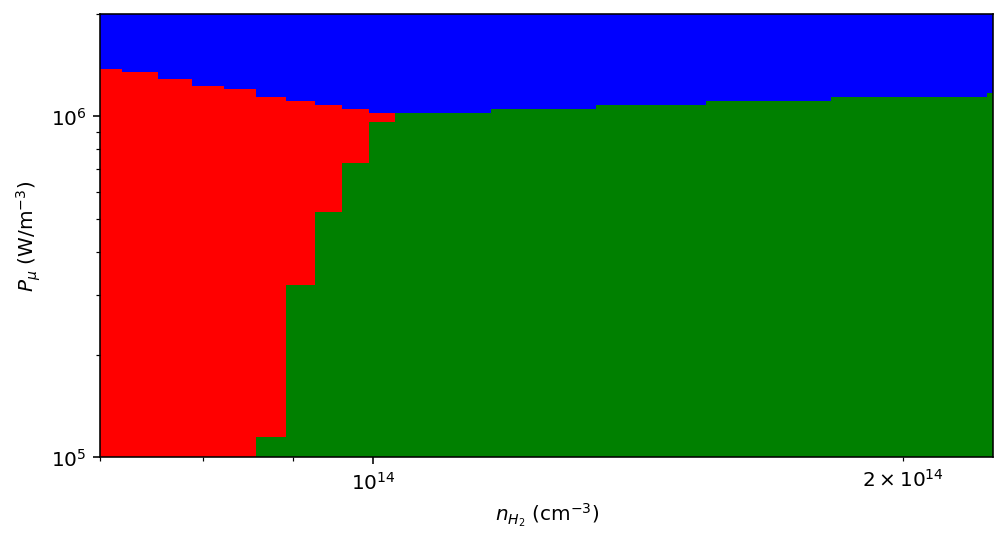
\includegraphics[width=0.7\linewidth]{2 - Oinarri teorikoa/predominant_volume.png}
    \caption{Espezie bakoitza (\colorbox{cyan}{$\mathbf{H_{ }^+}$}, \colorbox{red}{$\mathbf{H_2^+}$}, \colorbox{green}{$\mathbf{H_3^+}$}) gailentzen den zonaldeen mapa, potentzia-dentsitatearen eta gas-dentsitatearen arabera, $f=\num{0.5}$ izanik.}
    \label{fig:predominant}
\end{figure}

Hortaz, garrantzitsua da protoien sorkuntza maximizatzen duten balioak aukeratzea. \ref{fig:predominant} irudiaren arabera, $H^+$ espeziearen sorkuntza beste espezieena baino handiagoa izateko $P_\mu > \num{1.1}\cdot10^6 \; \frac{W}{m^3}$ eta $n_{H_2}>\num{1.1}\cdot10^{14}\;cm^{-3}$ izan behar dira. Balio minimo horien tresnetako baliokideak hurrengoak dira, \eqref{eq:potdentsitate} eta \eqref{eq:gasfluxu}  ekuazioak erabiliz,

\begin{equation}
\boxed{
    \begin{align}
        P_\mu &= \num{1.1}\cdot10^6 \frac{W}{m^3} \xRightarrow{} P_{eraso} \simeq 333 W \\
        n_{H_2} &= \num{1.1}\cdot10^{14}cm^{-3} \xRightarrow{} Q \simeq 5 sccm
    \end{align}
}
\end{equation}\\

Aldagai horiek finkatuko dira, potentzia gehiago handituz gero ganbararen tenperatura asko handitzen baita, eta gas-punpak ahalbidetzen duen fluxu maximoa hori baita. Orduan, sistema ebatziz gero, hurrengo espezieen dentsitateak lortzen dira,

\begin{equation}
\boxed{
    \begin{align}
        n_{H^+} = \num{3.1939} \cdot 10^{11} cm^{-3} \\
        n_{H_2^+} = \num{2.7243} \cdot 10^{11} cm^{-3} \\
        n_{H_3^+} = \num{2.9296} \cdot 10^{11} cm^{-3}\\
        n_{e^-} = \num{8.8478} \cdot 10^{11} cm^{-3}
    \end{align}
}
\end{equation}\\

Ikus daitekeenez, protoien dentsitatea ($\% \num{36.1}$) dihidrogeno katioiarena ($\% \num{30.79}$) eta trihidrogeno katioiarena ($\% \num{33.11}$) baino handiagoa da, maximizazio baldintza betez. Kostu konputazionala murrizteko simulazioetan 40000 partikula simulatzea erabaki denez, proportzioak errespetatuz \textbf{14440 $H^+$}, \textbf{12316 $H_2^+$} eta \textbf{13244 $H_3^+$} partikula simulatuko dira (\ref{sec:diseinusimulazio}. atala).

\subsection{Ioi-izpia}
Ioi-izpiak eta argi-izpiak kontzeptualki oso antzekoak dira, batez ere fotoiek eta partikula azpiatomikoek uhin-partikula dualtasuna partekatzen dutelako. Hori dela eta, ioi-izpien ibilbideak deskribatzeko optika klasikoaren formalismo matematikoa erabiltzen da, eta baita lenteen kontzeptua ere, ioien kasuan eremu elektriko eta magnetikoak erabiliz izpiaren fokuratze eta desfokuratzea lortzeko \cite{rose_geometrical_2012}. \\

Hala ere, desberdintasun nabarmenak existitzen dira horien artean. Argiaren kasuan, ingurune aldaketak bat-batekoak dira, eta baita errefrakzio-indizeen aldaketa ere. Ioi-optikan, ordea, ez dago ingurune aldaketarik, hutsa beharrezkoa baita, eta errefrakzioa eremu elektriko eta magnetikoen bidez ematen denez, errefrakzio-indize ez-konstante moduan jokatzen dute \cite{manura_simion_2008}. 

\subsubsection{Propietateak}
Ioi-izpien propietateei dagokienez, kargadun eta masadun partikulez osatuta daudela kontuan hartu behar da, argi-izpiak ez bezala. Testu honen analisirako beharrezkoak diren propietate nagusienak hiru dira: \textbf{intentsitatea}, \textbf{karga-espazioa} eta \textbf{emitantzia}.
\paragraph{Intentsitatea} \leavevmode\\

Izpiaren intentsitatea korronte-elektrikoaren baliokidetzat definitzen da \cite{scrivens_requirements_2014},

\begin{equation}
    I = q N_p
\end{equation}
\\
non $N_p$ azalera zeharkatzen duen batezbesteko partikula kopurua den, denbora-unitateko. Iturritik hainbat hidrogeno espezie erauzten direnez, partikula bakoitzarentzat intentsitate bat definitu daiteke, izpiaren intentsitate osoa horien batura izanik, \\
\begin{equation}
    I_{totala} = \sum_{j={H^+},{H_2^+},{H_3^+}}I_j = \sum_j qN_j
\end{equation}

Linac-7 proiektuan, intentsitatea \textit{Faraday Cup} baten bidez neurtzen da \cite{feuchtwanger_new_2022}.
\paragraph{Karga-espazioa}\leavevmode\\

Iturritik erauzitako partikulek karga zeinu berdina dutenez, elkar aldarapena jasaten dute indar Coulombdarren ondorioz, izpiaren dibergentzia handituz. Karga\hyp{}espazioaren efektua karga-dentsitatearen araberakoa da,

\begin{equation}
    \rho = \frac{J}{v}=\frac{I}{Av}
\end{equation}
\\
non $I$ intentsitatea, $A$ zehar-sekzioaren azalera eta $v$ izpiaren abiadura diren.\\

Geroz eta karga-dentsitatea handiagoa, orduan eta handiagoa da aldarapena. Dena den, azeleragailu honetan intentsitate baxuak neurtzen direnez ($10^{-6}A$), karga\hyp{}espazioaren eragina mespretxagarria dela onartzen da, simulazioen kostu konputazionala asko murriztuz.
\paragraph{Emitantzia}\leavevmode\\

Emitantziak ioi-izpi baten kalitatea kualitatiboki deskribatzeko oinarria ematen du. Tradizionalki, ($q,p$) koordenatu-kanonikoko 6N dimentsioko partikula\hyp{}dentsitateak fase-espazioan hartzen duen bolumena bezala definitzen da \cite{scrivens_requirements_2014}. Beraz, Liouvilleren teoremaren arabera,

\begin{equation}
    \frac{d\rho}{dt}=0
\end{equation}
\\
fase-espazioaren dentsitatea kontserbatzen denez, emitantzia kontserbatzen da; betiere indar kontserbakorren eraginpean eta karga-espazioaren eragina mespretxagarria bada. \\

Fase-espazioarekin lan egitea ez da oso praktikoa eta, partikulen elkarrekintzarik ez dagoela onartuz gero, ohikoagoa da aztarna-espazioa deiturikoa erabiltzea: izpia $x$-ardatzean hedatzen dela onartuz, plano bereko posizio eta ibilbidearen malda bikotea erabiltzea ($y,y'=\frac{dy}{dx}$)($z,z'=\frac{dz}{dx}$). Horrela, partikula guztien aldibereko aztarna-espazioen grafikoak irudikatuz, izpiaren dibergentzia edo konbergentziari buruzko informazioa lortu dezakegu, eta baita emitantziaren balioa azaleraren bitartez (\ref{fig:aztarna-espazio}. irudia).\\

\begin{figure}[h]
    \centering
    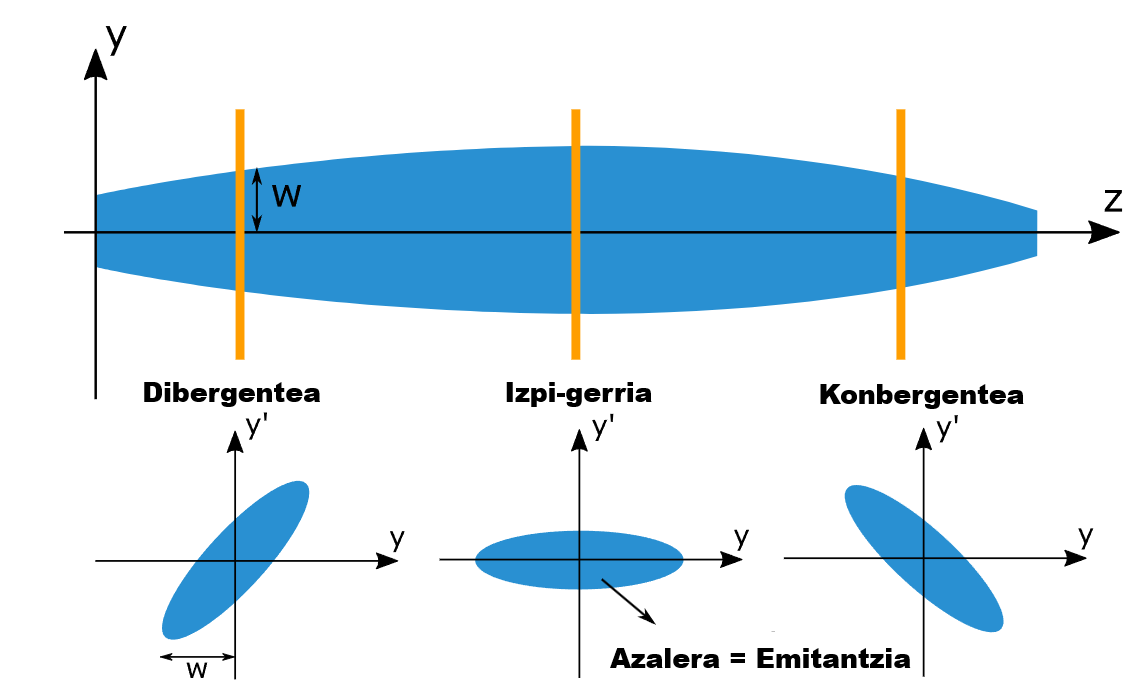
\includegraphics[width=0.9\linewidth]{2 - Oinarri teorikoa/trace_space.png}
    \caption{Ioi-izpi baten bilakaeraren eskema sinplea, zonalde bakoitzerako aztarna-espazioa irudikatuz.}
    \label{fig:aztarna-espazio}
\end{figure}

Hala ere, emitantziaren beste definizio orokorrago bat existitzen da, aztarna-espazioaren azalera ez dena, RMS-emitantzia deritzona \cite{reiser_theory_2007},

\begin{equation}
    \epsilon_{yy',rms}=\sqrt{\overline{y^2}\cdot\overline{y'^2}-\overline{yy'}^2}
\end{equation}
\\
non $\overline{y^2}$, $\overline{y'^2}$ eta $\overline{yy'}^2$ bariantzak diren. Azken terminoa partikularen posizioaren eta ibilbidearen arteko korrelazioa da, izpia dibergentea denean RMS-emitantziaren balioa handituz, eta alderantziz konbergentea denean. \\

Definizio honetarako, emitantzia ez dago normalizatuta, eta izpiaren momentuarekin aldatzen da; hortaz, emitantzia normalizatuta definitu daiteke:

\begin{equation}
    \epsilon_{yy',rms}^N=\beta \gamma \epsilon_{yy',rms}
\end{equation}
\\
non $\beta=\frac{v}{c}$ eta $\gamma=\frac{1}{\sqrt{1-\beta^2}}$ Lorentzen faktorea diren. Ez dago unitate definitu bakarrik emitantziarentzat, baina erabiliena $mm$ $mrad$ unitatea da \cite{becker_why_2006}.

\subsubsection{Erauzketa: lente elektrostatikoak}
\label{sec:lenteelektrostatiko}

PIT30 iturriko ioiak elektrodo baten bitartez erauzten dira ($V_{ext}$), eta izpiak zeharkatzen duen lehen elementua Einzel lente bat da: propagazio ardatzean ($x$) irekiera zilindrikoak dituzten hiru elektrodo, lehenengoa eta azkenengoa lurrera konektatuta, eta erdikoa, berriz, kasu honetan erauzketa-potentzialaren erdira finkatuta ($\frac{V_{ext}}{2}$).

\begin{figure}[h]
    \centering
    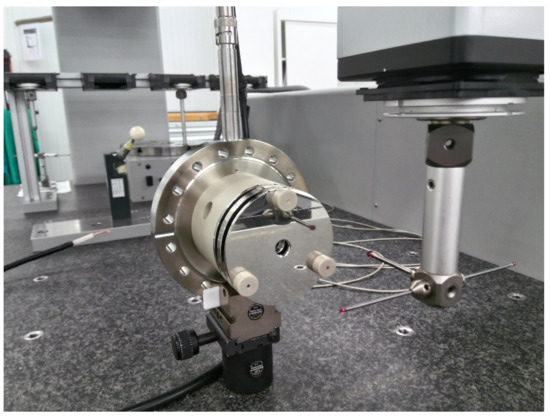
\includegraphics[width=0.45\linewidth]{2 - Oinarri teorikoa/einzel lens.jpg}
    \caption{Linac-7 proiektuan erabiltzen den Einzel lentea. \cite{feuchtwanger_new_2022}.}
    \label{fig:enter-label}
\end{figure}

Lente elektrostatikoen portaera ondo ulertzeko, ioi-optikan parte hartzen duten elementuen matrizeak emango dira, optika klasikoaren matrize formalismoa erabiliz. Simetria zilindrikoa dagoenez, $x$-ardatzeko edozein posiziorako partikula baten izpi bektorea honela definitzen da,\\

\begin{equation}
    \vec{r}(x)= \begin{pmatrix}
        r \\
        r' 
    \end{pmatrix} = 
    \begin{pmatrix}
        desplazamendu\; erradiala\\
        desbideraketa\; angeluar\; erradiala
    \end{pmatrix}
\end{equation}\\

Hortaz, sistema optiko bat zeharkatzerakoan, izpiaren koordenatu aldaketak $R(x)$ $2x2$ matrize baten bidez adieraz daiteke, garraio-matrizea deiturikoa. Einzel lenteak ulertzeko nahikoa da bi garraio-matrize definitzea: ioiek \textbf{eremu elektrostatiko uniforme} bat zeharkatzerakoan jasandakoa, eta ioiek \textbf{irekiera zilindrikoko elektrodo} batetik igarotzerakoan jasandakoa. Matrizeen garapen analitiko zehatza \ref{ap:matrizeak}. eranskinean aurki daiteke.

\paragraph{Eremu elektrostatiko uniformea}\leavevmode\\

$L$ distantziara dauden $V_1$ eta $V_2$ potentzialeko planoen artean $\vec{E}=E\cdot \hat{x}$ eremu-elektriko konstante bat sortzen da. Eremu hori zeharkatzen duen partikula baten ibilbidea hurrengo garraio-matrizearen arabera aldatuko da,

\begin{equation}
\boxed{
    R_U = \begin{pmatrix}
            1 & \frac{2L}{\sqrt{V_2/V_1}+1}\\
            0 & \sqrt{\frac{V_1}{V_2}}
    \end{pmatrix}
}
\end{equation}

Beraz, $V_1>V_2$ denean, protoiak azeleratzen dira, eta desbideraketa angeluar erradiala handitzen da. Bestalde, $V_2>V_1$ denean, alderantzizkoa gertatzen da. Gainera, $V_1=V_2$ bada, higidura askearen matrize klasikoa berreskuratzen da.

\paragraph{Irekiera zilindrikoko elektrodoak}\leavevmode\\

Praktikan, ordea, ioiek ez dituzte potentzial planoak zeharkatzen, baizik eta potentzial horiek dituzten elektrodoetako irekieretatik igarotzen dira. Irekiera horien inguruan, gainazal-ekipotentzialak kurbatzen dira, eremu-elektrikoaren osagai erradialak sartuz. Hori dela eta, irekierek lente moduan jokatzen dute, eta garraio\hyp{}matrizea hurrengoa da,

\begin{equation}
\boxed{
    R_A = \begin{pmatrix}
            1 & 0\\
            \frac{q(E_1-E_2)}{2mv_x^2} & 1
    \end{pmatrix}
}
\end{equation}
\\
non $E_1$ eta $E_2$ irekieraren ezker eta eskuinaldeko eremu elektrikoak diren, hurrenez hurren. Matrize hori argi lente klasiko baten garraio-matrizearekin alderatuz \cite{liebl_applied_2008}, lente elektrostatikoen foku-distantzia lortu dezakegu,

\begin{equation}
    R_{lente}=\begin{pmatrix}
        1 & 0\\
        -\frac{1}{f} & 1
    \end{pmatrix} \quad \Longrightarrow \quad f=\frac{2mv_x^2L}{q(E_2-E_1)}
\end{equation}\\

Beraz, $E_1>E_2$ denean, distantzia fokala negatiboa da, irekiera lente dibergente moduan jokatuz; $E_2>E_1$ denean, ordea, distantzia fokala positiboa da, lente konbergente moduan jokatuz.
\paragraph{Einzel lenteak}\leavevmode\\

\ref{sec:lenteelektrostatiko} ataleko sarreran aipatu den moduan, Einzel lenteak irekiera zilindrikoko hiru elektrodoz osatutako sistemak dira. Garatutako formalismoaren arabera, honela ikus daitezke (\ref{fig:einzeleskema}. irudia):

\begin{center}
    \textbf{\textit{1.irekiera~$\Rightarrow$~1.eremu unif.~$\Rightarrow$~2.irekiera~$\Rightarrow$~2.eremu unif.~$\Rightarrow$~3.irekiera}}
\end{center}

Garraio-matrizea honela adierazi daiteke,

\begin{equation}
\boxed{
    R_{einzel}=R_{A1}\cdot R_{U1}\cdot R_{A2}\cdot R_{U_2} \cdot{R_{A3}}
}
\end{equation}

Gainera, elektrodoen potentzialak $V_1-V_2-V_1$ direnez, $V_2>V_1$ izanik, honela jokatzen dute:

\begin{center}
    \textbf{\textit{lente dib.~$\Rightarrow$~dezelerazioa~$\Rightarrow$~lente konb.~$\Rightarrow$~azelerazioa~$\Rightarrow$~lente dib.}}
\end{center}

Diseinu simetrikoari esker, izpiaren lehenengo kolimazioa burutu daiteke partikulen energia aldatu gabe.

\begin{figure}[h]
    \centering
    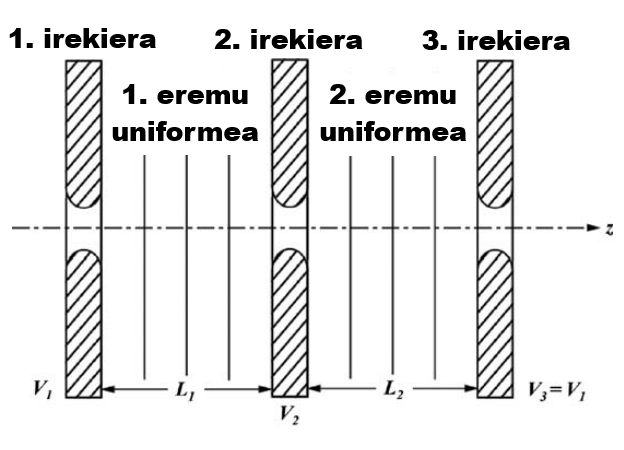
\includegraphics[width=0.6\linewidth]{2 - Oinarri teorikoa/einzel_lens_scheme.png}
    \caption{Einzel lente baten eskema, elementu sinpleagoetan zatituta.}
    \label{fig:einzeleskema}
\end{figure}

\subsection{Wien Filter-a}
Einzel lentetik igarotzean partikulen energia aldatzen ez denez, erauzitakoan emandako energia berdina dute ($E_k=q\Delta V_{ext}$). Hala ere, espezie desberdinek karga berdina eta masa desberdina dutenez, abiaduraren arabera desberdindu ditzakegu. PIT30 iturriaren erauzte-potentzialaren balio nominala $V_{ext}=30\;kV$ izanik,

\begin{equation}
    \frac{1}{2}m_iv_i^2=qV_{ext} \quad \Longrightarrow v_i =\sqrt{\frac{2qV_{ext}}{m_i}} \quad \Longrightarrow \quad \boxed{ \begin{aligned}
        H^+: \quad & v_{H^+}=\num{2.398}\cdot10^6\quad m/s\\
        H_2^+: \quad & v_{H_2^+}=\num{1.695}\cdot10^6\quad m/s \\
        H_3^+: \quad & v_{H_3^+}=\num{1.384}\cdot10^6\quad m/s
\end{aligned}
}
\end{equation}\\

\textit{Wien Filter}-en bitartez posiblea da partikula baten abiadura hautatzea, eremu elektriko eta magnetikoen bidez, honek indarrik ez jasateko eta beste espezieak desbideratzeko. Eremuak izpiaren hedatze-ardatzarekiko perpendikularrak aukeratuz, beti aurki daitezke bi norabide, euren artean perpendikularrak ere, partikulek jasandako indarrak aurkakoak izateko. Adibidez, izpia $+x$-ardatzean hedatzen dela onartuz, eremu elektrikoa ($E$) $+y$-ardatzean finkatuz, eta eremu magnetikoa ($B$) $+z$-ardatzean finkatuz gero (\ref{fig:enter-wieneskema}. irudia),

\begin{equation}
    \left.
    \begin{aligned}
        \vec{F_e}&=q\vec{E}=qE\cdot \hat{y} \\
        \vec{F_m}&=q (\vec{v}\times \vec{B})=qvB(\hat{x}\times \hat{z})=qvB\cdot(-\hat{y})
    \end{aligned}
    \right\}
     \Longrightarrow \vec{F}_{net}=\sum_j F_j=q(E-vB) \cdot \hat{y}
     \label{eq:prewien}
\end{equation}\\

Hortaz, pasatzen utziko den partikularen abiadura ($v_f$) hautatzeko, indarrik jasan behar ez duenez, honelakoa da \textbf{\textit{Wien} baldintza},

\begin{equation}
    \vec{F_{net}}=q(E-v_fB)\cdot {\hat{y}}=0 \quad \Longrightarrow \quad \boxed{v_f = \frac{E}{B}}
    \label{eq:wienproperty}
\end{equation}\\
\begin{figure}[h]
    \centering
    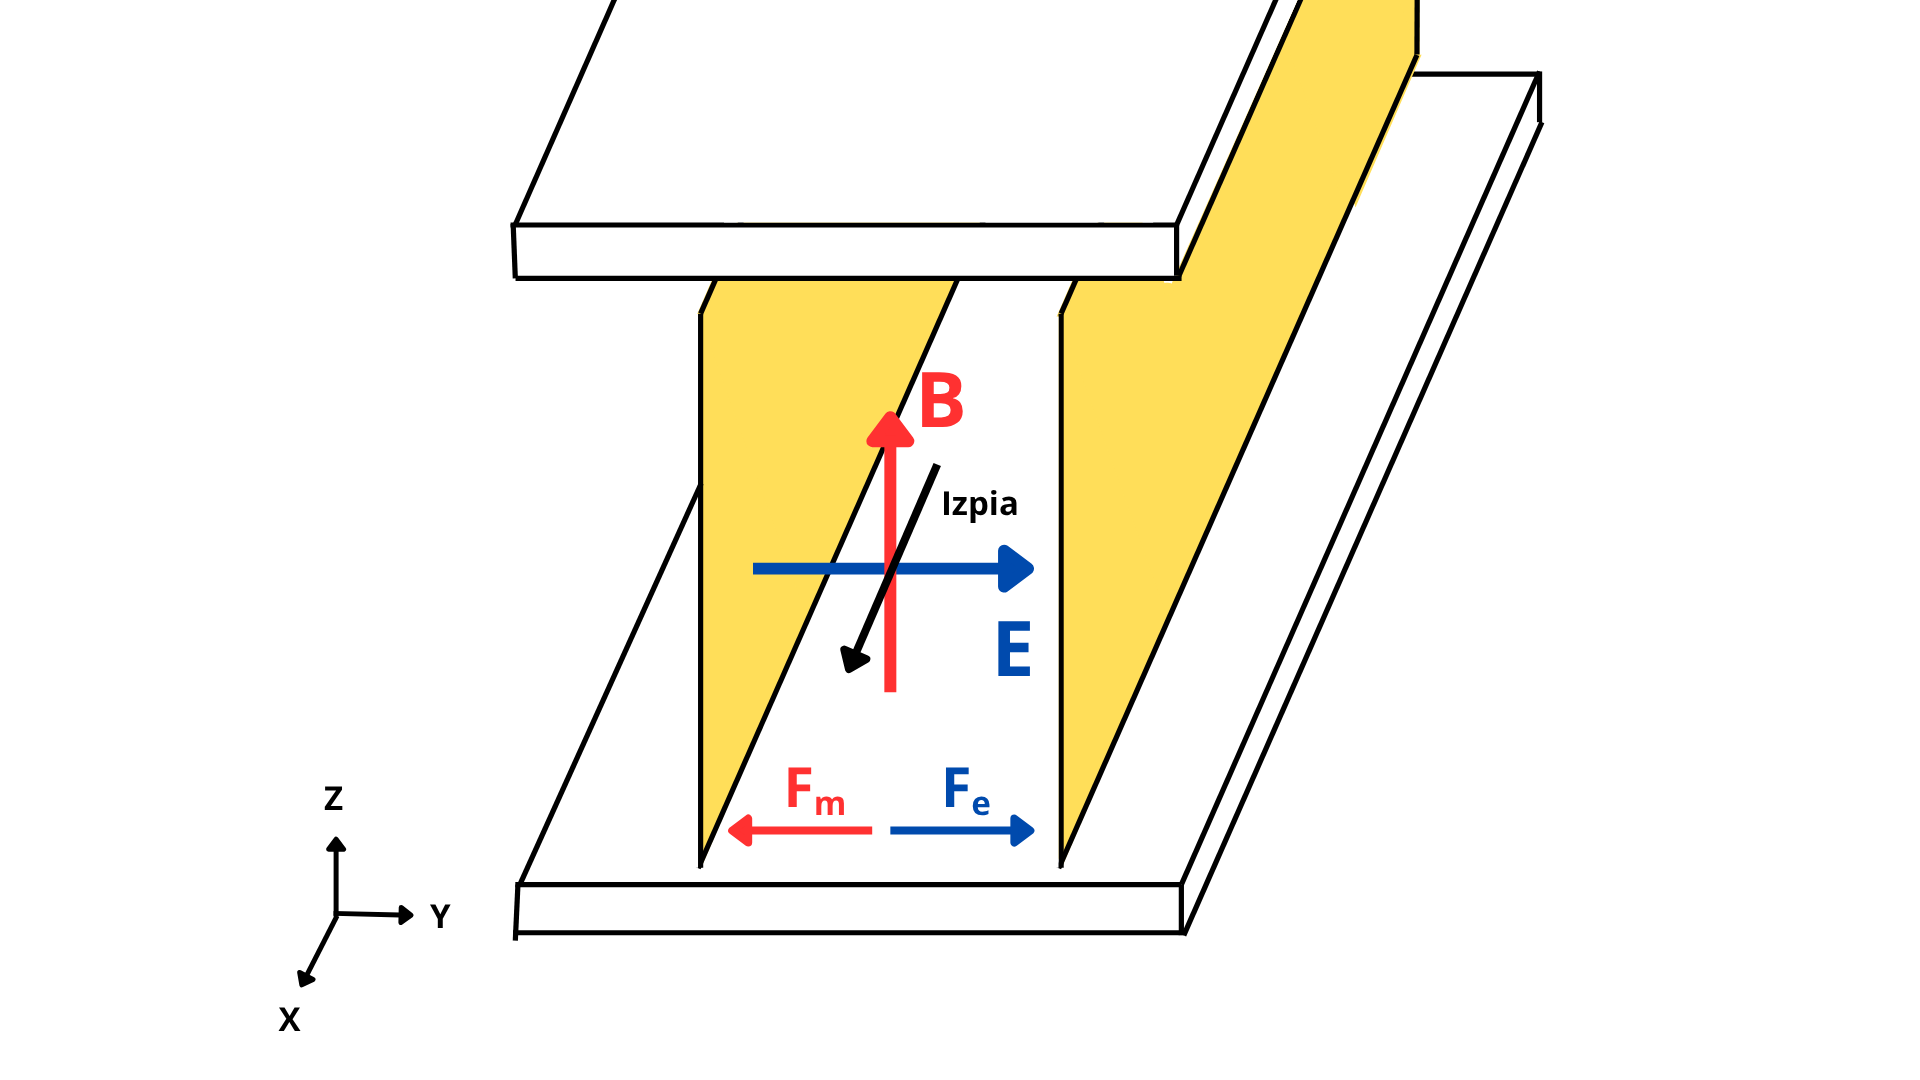
\includegraphics[width=0.9\linewidth]{2 - Oinarri teorikoa/wienfilter_eskema.png}
    \caption{\textit{Wien Filter} baten eskema sinplifikatuta.}
    \label{fig:enter-wieneskema}
\end{figure}

\textit{Wien Filter}-en diseinuan oso garrantzitsua da eremuen aukeraketa; izan ere, Wien baldintza hautatutako partikularen abiadurarekin guztiz bat ez badator, partikulek indarrak jasango dituzte, izpiaren kalitateari eraginez. Ondorioz, ahalik eta eremu uniformeenak lortzea ezinbestekoa da.

\subsubsection{Eremu elektrikoa: elektrodo paraleloak}
\label{sec:elektrodo_paraleloak}

Eremu elektrikoaren kasuan, ohikoa da bi xafla eroale, lau eta paralelo erabiltzea eremu uniformeko zonalde bat sortzeko. Kalkuluak errazteko infinitua, laua eta uniformea dela onartuz, $\sigma$ gainazal-karga duen xafla batek sortutako eremu elektrikoa, Gaussen legearen arabera \cite{griffiths_introduction_1999},\\

\begin{equation}
\vec{E}=\frac{\sigma}{2\epsilon_0}\hat{n}
\end{equation}
\\
non $\hat{n}$ gainazalaren bektore-normal unitarioa eta $\epsilon_0$ hutsaren permeabilitatea diren. Orduan, aurkako gainazal-karga ($+\sigma , -\sigma$) duten bi xafla aurrez-aurre $d$ distantziara jarriz gero (\ref{fig:eroaleparalelo}. irudia), xaflen arteko eremutik kanpoko eremuak elkar deuseztatzen dira, eta bien arteko zonaldeko eremua, berriz,

\begin{equation}
    \vec{E} = \frac{\sigma}{\epsilon_0}\hat{n}
\end{equation}

Gainera, eroaleen gaineko potentzial elektrikoa (V) konstantea denez, bi eroaleen arteko potentzial-diferentzia eremu elektrikoarekin erlaziona daiteke,

\begin{equation}
    \Delta V = V_{+} - V_{-} = -\int_{-}^+ \vec{E} \cdot d \vec{l} \quad \Longrightarrow \quad  \boxed{E=\frac{\Delta V}{d}}
    \label{eq:eremue_paralelo}
\end{equation}

\begin{figure}[h]
    \centering
    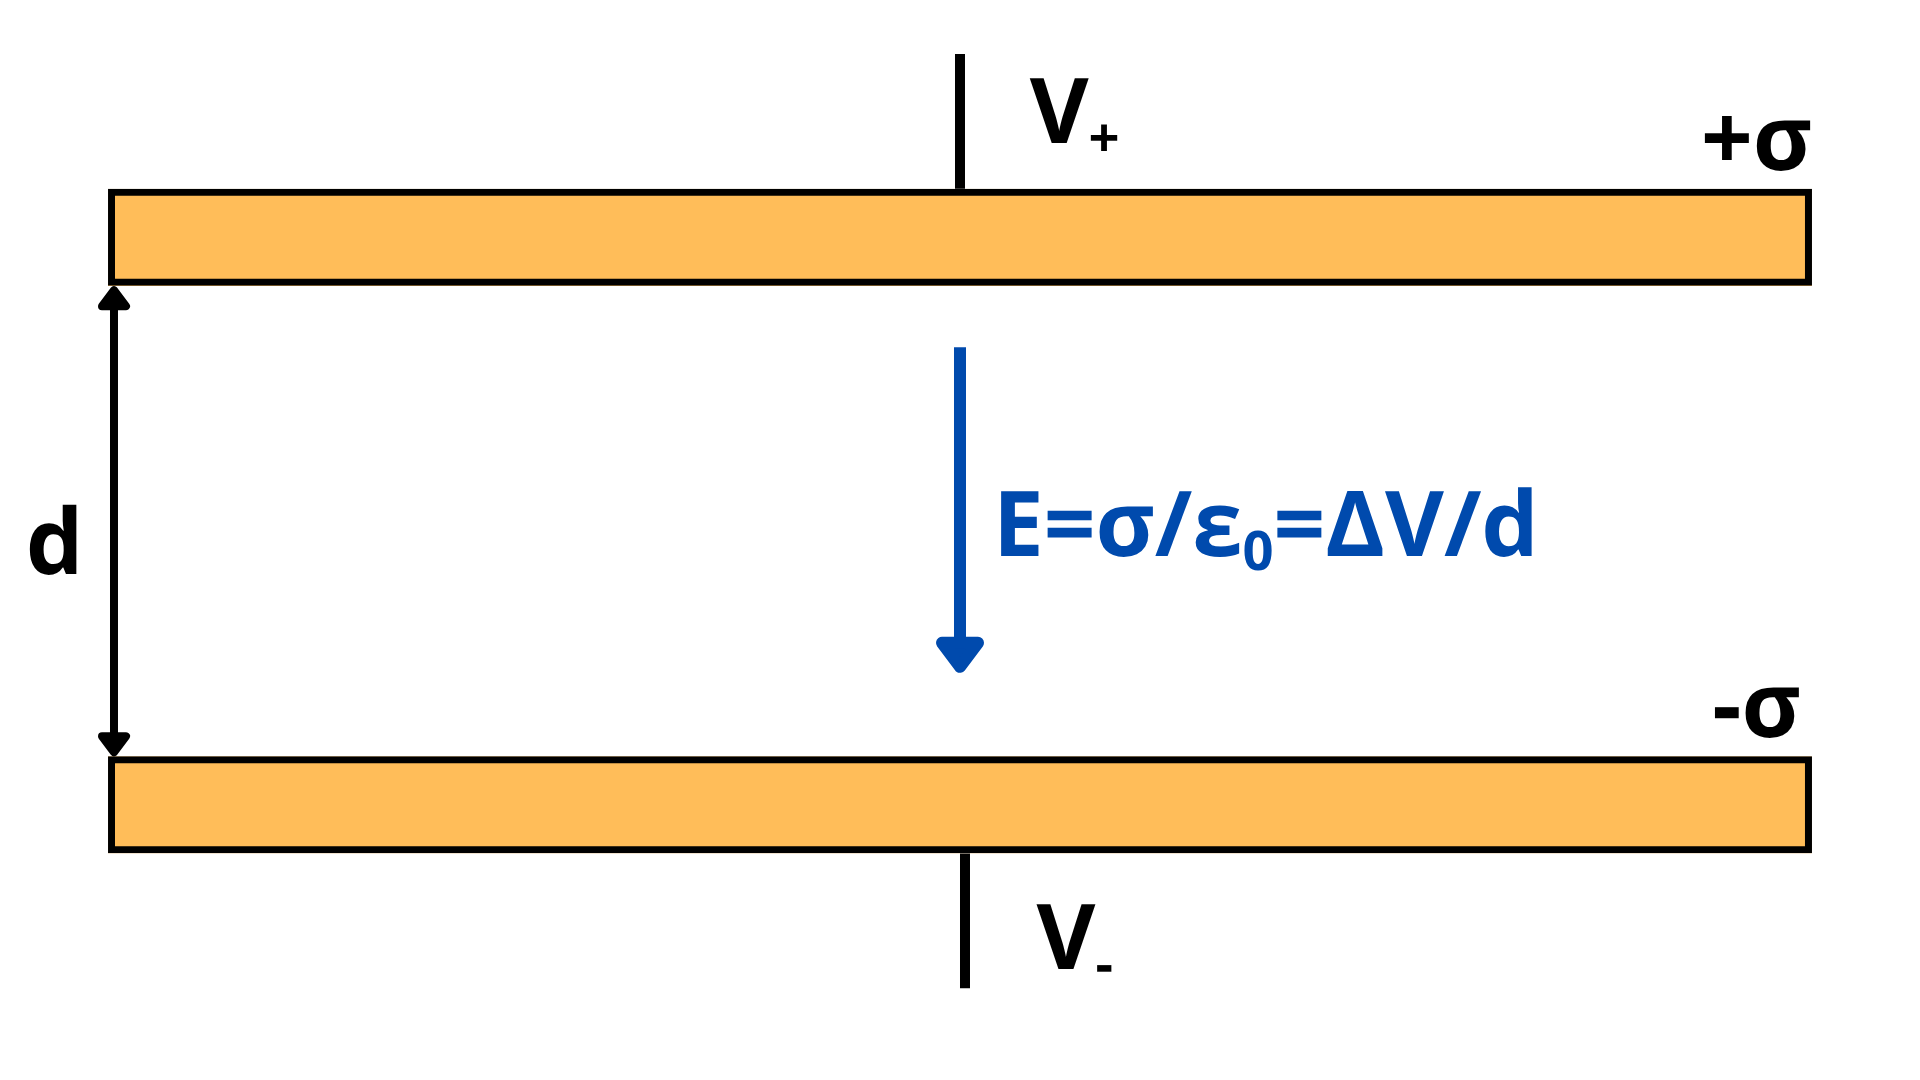
\includegraphics[width=0.7\linewidth]{2 - Oinarri teorikoa/parallel_plate.png}
    \caption{Bi xafla eroale, lau eta paraleloen arteko eremu-elektrikoa.}
    \label{fig:eroaleparalelo}
\end{figure}

Horrela, xaflen arteko distantzia eta potentzialak zehaztuz, Wien baldintza betetzeko beharrezko eremu elektrikoa sortu daiteke. Hala ere, errealitatean xaflak ezin dira infinitoak izan, eta lortutako adierazpenak ertzetan ez dira betetzen. \textbf{Ertz-efektuak} oso garrantzitsuak dira \textit{Wien filter}-en diseinuan, baldintza edozein puntutan betetzea ezinbestekoa baita, eta diseinuaren atalean horietan sakonduko da (\ref{sec:diseinu-finala}. atala).
\subsubsection{Eremu magnetikoa: iman iraunkorrak}
\label{sec:iman_iraunkorrak}

Eremu magnetiko uniformeko zonalde bat sortzeko, ordea, ohikoa da iman iraunkorrak erabiltzea, batez ere oso merkeak direlako, eta elikadura behar duten elektroimanen edo solenoideen erabilera saihesteko. \textit{Wien Filter}-etan erabiltzen diren iman iraunkor gehienak material ferromagnetiko gogorrez osatuta daude, beren indukzio magnetiko erremanente ($B_r$) handiari esker.\\

Bloke laukizuzen batek bere inguruan sortzen duen eremu magnetikoa kalkulatzea ez da erraza; blokearen neurrien, materialaren eta magnetizazio norabideren araberakoa da. Hortaz, ohikoa da ordenagailuzko simulazioak erabiltzea horiek lortzeko. Dena den, \textit{supermagnete} \cite{noauthor_calcular_nodate} fabrikatzaileak formula hau eskaintzen du,

\begin{equation}
    B = \frac{B_r}{\pi}[\arctan(\frac{LW}{2z\sqrt{4z^2+L^2+W^2}})- \arctan(\frac{LW}{2(D+z)\sqrt{4(D+z)^2+L^2+W^2}})]
\end{equation}
\\
non $L$, $W$ eta $D$ imanaren luzera, zabalera eta altuera diren, hurrenez hurren, eta $z$, berriz, gainazal polar baten simetria-ardatzarekiko distantzia (\ref{fig:bloke_magnetiko}. irudia).\\

Eremu elektrikoen analogiaz, eremu magnetiko uniformeko zonaldeak sortu daitezke bi iman iraunkorrekin: aurkako poloak aurrez-aurre jarrita, eremu-lerroak baten ipar polotik atera eta bestearen hego polotik sartuko dira. Horrela, imanen arteko distantzia aurpegien azalerarekiko behar bezain txikia bada, eremu magnetiko uniforme bat lortu daiteke.

\begin{figure}[h]
  \centering
  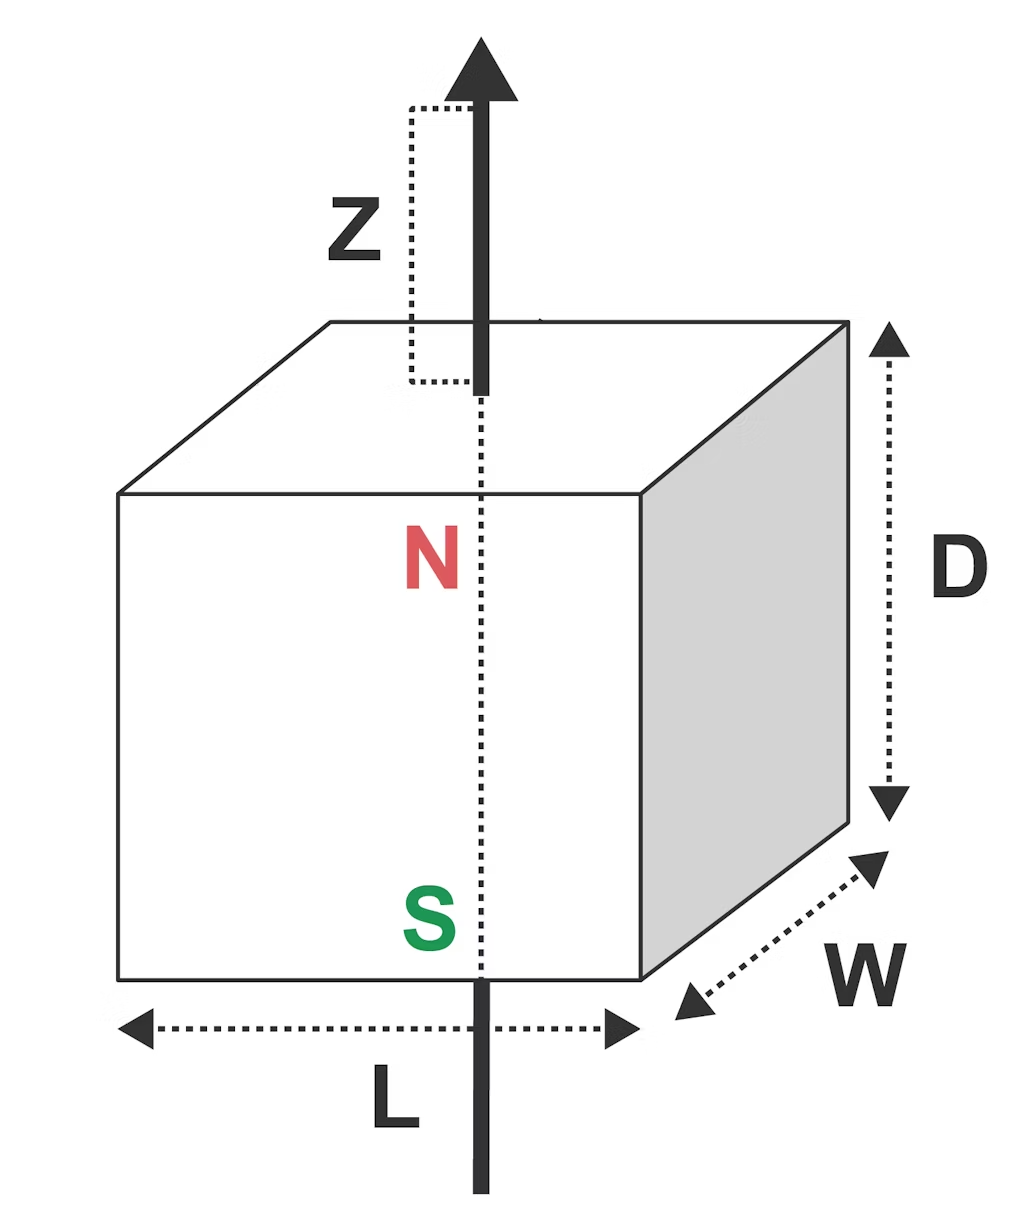
\includegraphics[width=0.35\textwidth]{2 - Oinarri teorikoa/magnetic_formula.png}
  \caption{Iman laukizuzen baten neurriak, $z$-norabidea magnetizazio norabidea izanik.}  \label{fig:bloke_magnetiko}
\end{figure}
\newpage
\subsubsection{Desbideraketa minimoa}
Baldintza mekanikoak betetzeko neurri batzuk aukeratu daitezke. Neurri horiek zehaztuta eta partikula baten abiadura aukeratuta, beste espezie bat irteerako erradiotik guztiz desbideratzeko beharrezko eremu minimoak kalkulatu daitezke. Dena dela, iragazkiaren diseinua prozesu iteratibo bat da, eta kalkulatutako eremuaren balioak onargarriak ez badira, diseinu mekanikoa aldatu beharko da. Luzera ($L$), sarrera erradioa ($r_{in}$) eta irteera erradioa ($r_{out}$) izanik (\ref{fig:desbideraketa_eskema}. irudia),

\begin{equation}
    \begin{aligned}
        v_i = \frac{L}{t_i} \quad \Longrightarrow& \quad t_i =\frac{L}{v_i}\\
        d_{y,i} = 2r_{out}+(r_{in}-r_{out}) \quad \Longrightarrow& \quad d_{y,i} =r_{in}+r_{out}= \frac{1}{2}a_{y,i}t_i^2
    \end{aligned}
    \label{eq:minimo}
\end{equation}
\\
non $d_{y,i}$ partikularen desbideraketa minimoa den, eta $t_i$ partikulak dispositiboan ematen duen denbora. Gainera, azelerazioa indarrak ere ematen duenez,

\begin{equation}
    m_i a_{y,i}=q(E-v_iB) \quad \Longrightarrow \quad a_{y,i}=\frac{q(E-v_iB)}{m_i}
\end{equation}
\\
eta \ref{eq:minimo} ordezkatuz, Wien baldintza (\ref{eq:wienproperty}) erabiliz eremu batentzat askatu daiteke,

\begin{equation}
    \frac{2(r_{in}+r_{out})v_i^2}{L^2}=\frac{q}{m_i}E(1-\frac{v_i}{v_f}) \quad \Longrightarrow \quad \begin{aligned}
        E&=\frac{2m_iv_i^2(r_{in}+r_{out})}{qL^2(1-\frac{v_i}{v_f})}\\
        B&=\frac{E}{v_f}=\frac{2m_iv_i^2(r_{in}+r_{out})}{qL^2(1-\frac{v_i}{v_f})v_f}
    \end{aligned}
\end{equation}

Azkenik, energia zinetikoa erauzketakoa dela onartuz, $\frac{1}{2}m_iv_i^2=qV_{ext}$,

\begin{equation}
    \boxed{
    E=\frac{4V_{ext}(r_{in}+r_{out})}{L^2(1-\frac{v_i}{v_f})} \hspace{1cm} B=\frac{4V_{ext}(r_{in}+r_{out})}{L^2(1-\frac{v_i}{v_f})v_f}
    }
    \label{eq:desbiderapena}
\end{equation}

Horrela, aukeratutakoa ez den partikula bat guztiz desbideratzeko eremu minimoa lortzen da. Hiru hidrogeno espezie izanik, aukeratutako bakoitzerako bi eremu minimo daude, eta beti handiena hartu behar da, beste biak guztiz iragazteko. 
\begin{figure}[h]
    \centering
    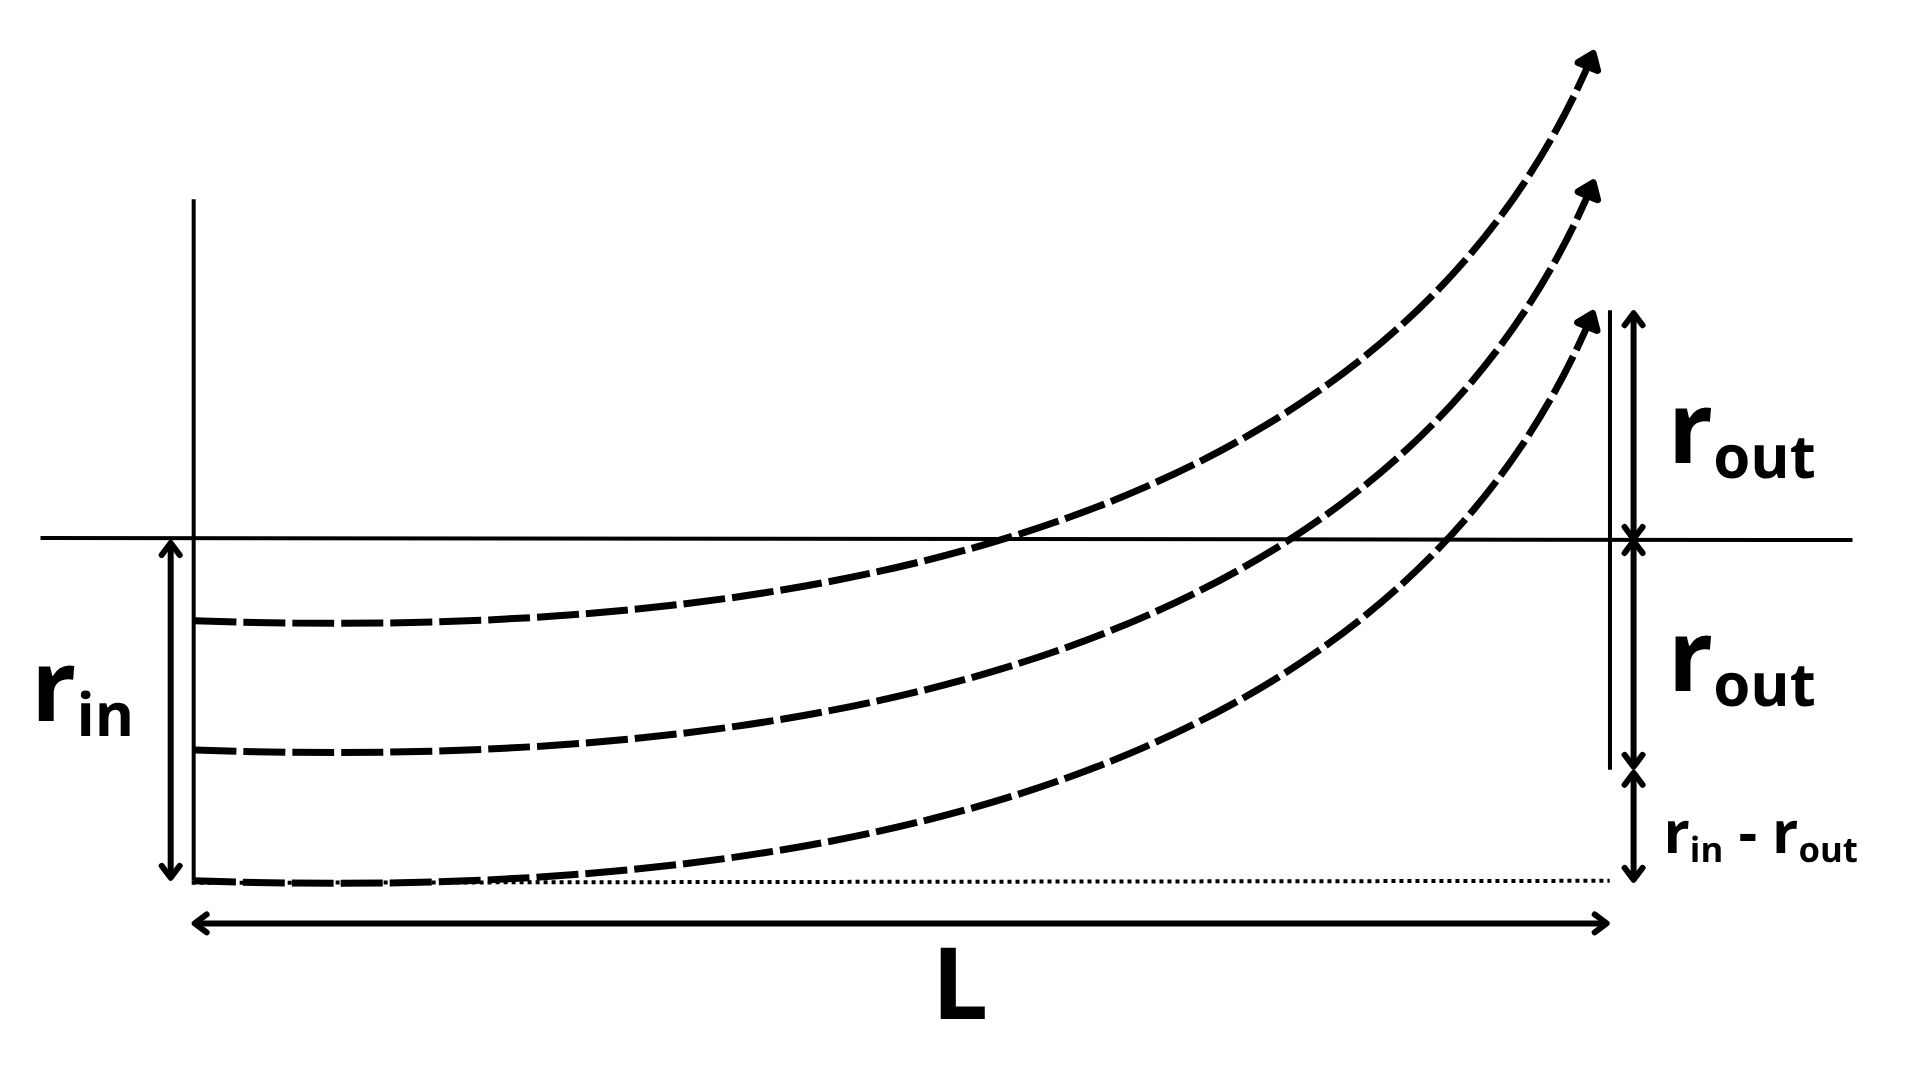
\includegraphics[width=0.5\linewidth]{2 - Oinarri teorikoa/desbideraketa_eskema.png}
    \caption{Partikula baten desbideraketaren eskema sinplea.}
    \label{fig:desbideraketa_eskema}
\end{figure}
\newpage
\section{COMSOL Multiphysics}
Iturritik erauzitako ioiak teorian ikusitako dispositiboetan duten portamoldea analizatzeko ordenagailuzko simulazioak oso lagungarriak dira. Orain arte, Linac-7 proiektuan SIMION erabili da, partikula kargadunen ibilbideen simulazioan espezializatutako softwarea \cite{noauthor_simion_2020}. Oraingoan, ordea, \textit{Wien Filter}-a diseinatzeko eta simulatzeko COMSOL Multiphysics \cite{noauthor_comsol_2025} softwarea erabiltzea erabaki da.
\subsection{Software Konparaketa}
\paragraph{SIMION}\leavevmode\\

SIMION-ek ioi-optikako simulazioetarako bi edo hiru dimentsioko espazio bat definitzen du, eta erabiltzaileak zehaztutako elementu infinitesimaletan banatzen da. Honi \textbf{potentzial-matrizea} deritzo, eta horren elementuek potentzial elektrostatiko edo magnetostatiko bat dute. Bi motako elementuak existitzen dira: elektrodoak eta ez-elektrodoak. Programatik kanpo sortutako artxibo bat erabiliz, elektrodoen geometria zehazten da, eta horien potentzialak zehazten dira. Ez\hyp{}elektrodoentzat, potentzialak Laplaceren ekuazioa ($\nabla^2V=0$) diferentzia finituen bidez ebatziz lortzen dira (\textit{potential refining}).

\begin{figure}[h]
    \centering
    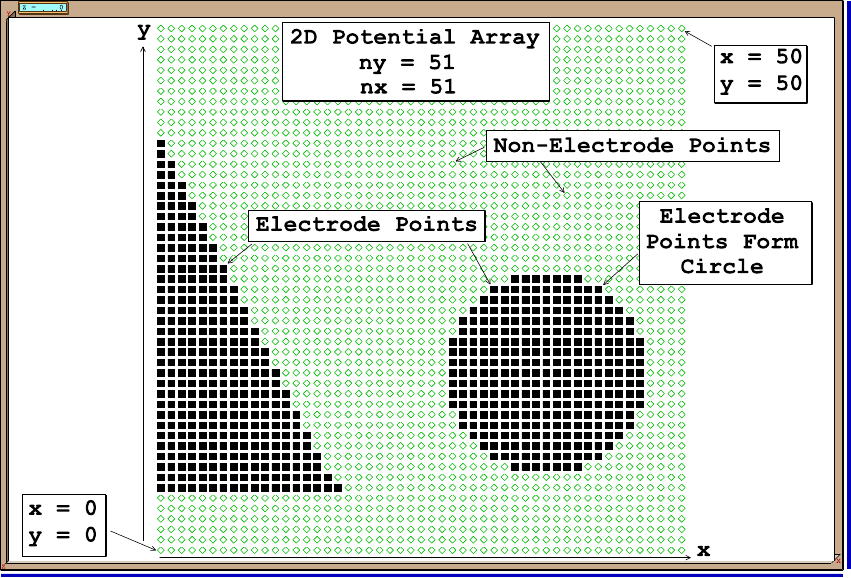
\includegraphics[width=0.6\linewidth]{3 - COMSOL/potential_array.png}
    \caption{Potentzial-matrize baten adibidea 2D-n \cite{manura_simion_2008}.}
    \label{fig:potential_array}
\end{figure}

Bestalde, simulazioan parte hartuko duten partikulak definitu behar dira. Taldeka definitu daitezke, partikula kopurua, banaketa distribuzioa, masa, karga, hasierako abiadura eta norabidea zehaztuz. Partikula bakoitzaren ibilbidea simulatzeko, SIMION-ek Runge-Kutta 4 erabiltzen du hurrengo pausuko posizioa eta abiadura lortzeko, potentzial-matrizetik lortutako eremuek emandako Lorentzen indarra kontuan hartuta.\\

Abantaila ugari eskaintzen ditu: programazio aldetik oso pertsonalizagarria da Lua programazio lengoaiari esker; aldagai ugari doitu daitezke, eta baita emitantzia bezalako magnitudeak kalkulatu. Mugapenak ere baditu: simulazioen ebazpena ez dago simetriarik gabeko sistementzat optimizatuta, eta horiek gauzatzeko denbora nabarmen handitzen da.
\newpage

\paragraph{COMSOL Multiphysics}\leavevmode\\

COMSOL Multiphysics elkarrekintza fisiko konplexuak simulatzea ahalbidetzen duen softwarea da, Elementu Finituen Metodoaz (FEM) baliatuz. Horren interfaze intuitibo eta optimizazio handiari esker, \textit{Wien Filter}-ak bezalako simetriarik gabeko sistemak modu eraginkorragoan simulatzea posiblea da. Erabiltzaileak geometria programan bertan definitzen du, eta baita geometria elementu bakoitzari esleitutako materiala ere (\ref{fig:comsol_geometry}. irudia).

\begin{figure}[h]
    \centering
    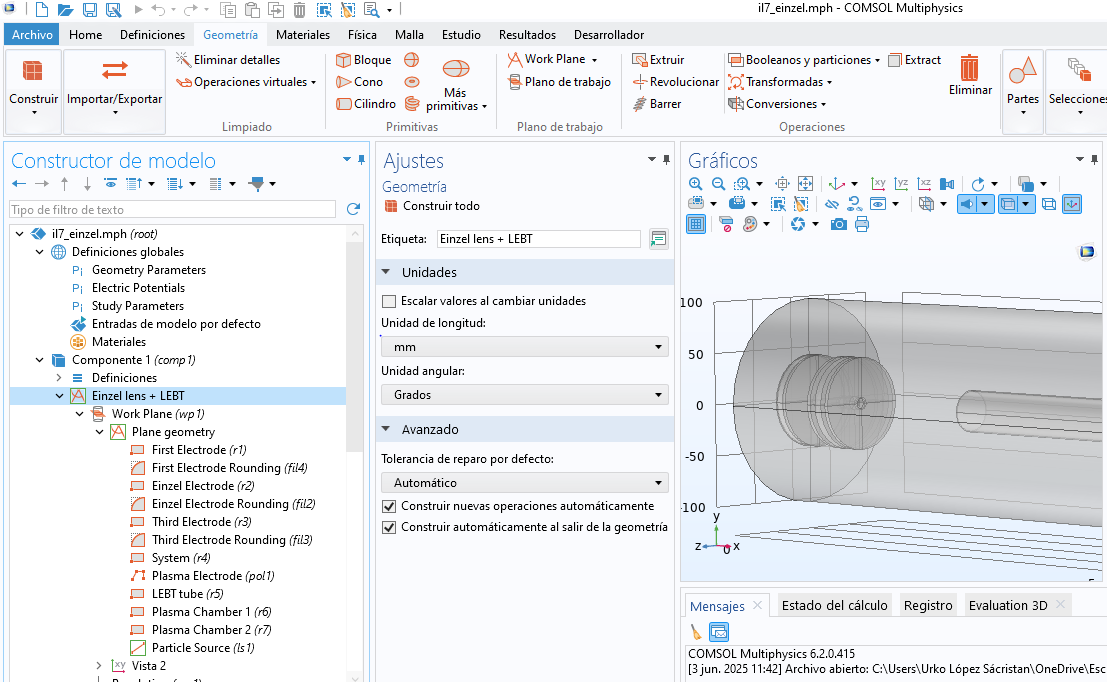
\includegraphics[width=0.85\linewidth]{3 - COMSOL/comsol_geometry.PNG}
    \caption{COMSOL Multiphysics-en interfaze nagusia. Ezkerrean, modeloa eraikitzeko beharrezko osagaiak; eskuinean, sistema osoaren 3D-ko ikuspegia.}
    \label{fig:comsol_geometry}
\end{figure}

Sistemarentzat beharrezkoak diren fisikak moduluen bidez inplementatzen dira. Kasu honetan, bi modulu dira beharrezkoak: \textbf{AC/DC modulua} eta \textbf{Partikula-Ibilbideen modulua} (\textit{Particle Tracing Module}). Horiek ebazteko, geometriak \textbf{sareetan} (\textit{\textbf{mesh}}) banatzen dira, elementu finituetan diskretizatuz, eta bakoitzerako ekuazio diferentzialak ebazten dira. Hainbat sare definitu daitezke, zehaztasuna elementuaren arabera doituz.

\begin{itemize}
    \item \textbf{AC/DC modulua:}  Eremu elektriko eta magnetikoak definitzeko aukera ematen du. Kasu honetan, eremu elektrikoak sortzeko, elektrodoen potentzialak eta lurrak zehazten dira; iman iraunkorrentzat, ordea, nahikoa da geometriari materiala esleitzea eta iman bezala definitzea, poloak aukeratuz. Horrela, materialaren propietateak erabiliz, solidoentzako Ampereren legea ebazten da, eremu magnetikoa lortuz.\\
    \item \textbf{Partikula-Ibilbideen modulua:} Hainbat partikulen propietateak definitzeko aukera eskaintzen du. Horiekin partikula-izpiak definitzen dira, hasierako posizioa, emitantzia, energia eta norabidea zehaztuz. Gainera, partikulen indarrak zehazten dira ere, beste moduluaz kalkulatutako edo eskuz sartutako eremuen arabera.\\
\end{itemize} 

Linac-7 proiektuan lortutako izpiaren intentsitatea baxua denez ($\sim 10^{-6}A$), karga-espaziorik ez dagoela onartuko dugu. Horrela, lehenik AC/DC modulua simulatuko da, eremuen soluzio geldikorra lortzeko, eta ondoren, soluzio geldikor horiek baliatuz, partikulen ibilbideak simulatuko dira. Bi moduluak independenteki ebazteak kostu konputazionala asko murrizten du. Nolanahi ere, nahi izanez gero karga-espazioa kontuan hartu daiteke bi moduluak aldi berean simulatuz.

\subsection{Sistemaren balidazioa}
\textit{Wien Filter}-aren diseinuarekin hasi baino lehen, COMSOL-en egindako simulazioak zuzenak direla egiaztatzea funtsezkoa da. Erauzketa sistemaren SIMION-eko simulazioetan lortutako emaitzak \cite{bermejillo_seco_optical_2021} COMSOL-en lortutakoekin konparatuko dira, eta bateragarriak badira, sistema fidagarritzat hartuko da.\\

Lehenik eta behin, erauzte-elektrodoaren eta Einzel lentearen elektrodoen geometria sortu dira. Sistemak biraketa-simetria duenez, geometria plano batean definitzeko eta biraketa bidez osatzeko aukera ematen du COMSOL-ek (\ref{fig:erauzketa_sistema}. irudia). 

\begin{figure}[h]
    \centering
    \begin{subfigure}[b]{0.6\textwidth}
        \centering
        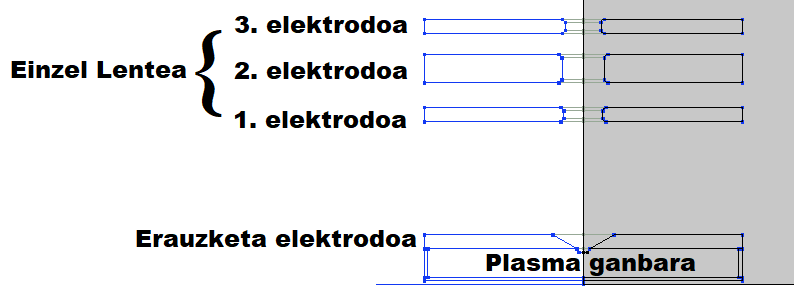
\includegraphics[width=\linewidth]{3 - COMSOL/extraction_plane.png}
        \caption{Planoan.}
        \label{fig:3d_plane}
    \end{subfigure}
    \hspace{0.02\textwidth}
    \begin{subfigure}[b]{0.26\textwidth}
        \centering
        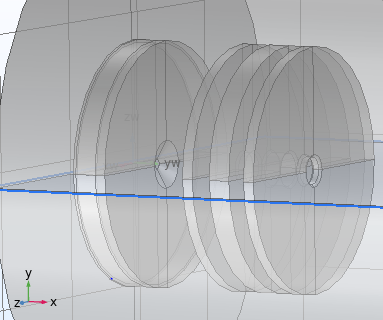
\includegraphics[width=\linewidth]{3 - COMSOL/extracion_3d.PNG}
        \caption{3D-n (biraketaz).}
        \label{fig:3d_extraction}
    \end{subfigure}
    \caption{Erauzketa sistemaren geometria.}
    \label{fig:erauzketa_sistema}
\end{figure}

Ondoren, AC/DC moduluaz elektrodoen tentsioak finkatu dira: $V_{ext}=30\;kV$ erauzketa-elektrodoan, $V_2=15\;kV$ lentearen erdiko elektrodoan, eta $V_1=V_3=0$ besteetan. Horrela, eremu elektrikoaren soluzio geldikorra lortu da (\ref{fig:eremugeldikor}. irudia).

\begin{figure}[h]
    \centering
    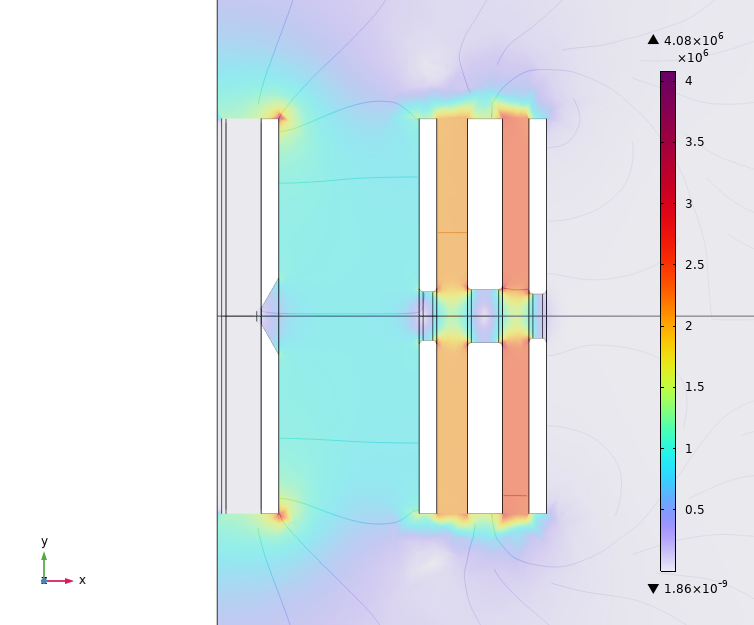
\includegraphics[width=0.5\linewidth]{3 - COMSOL/eremu_elektrikoa.png}
    \caption{Eremu elektriko geldikorra ($V_{ext}=30\;kV$, $V_2=15\;kV$, $V_1=V_3=0$).}
    \label{fig:eremugeldikor}
\end{figure}

Azkenik, partikula-izpia definitzeko \ref{sec:plasma} atalan aipatutako konfigurazioa erabili da: 40000 partikula, horietatik 14440 $H^+$, 12316 $H_2^+$ eta 13244 $H_3^+$, hasierako posizioek $r=\num{1.2}\;mm$ erradioko banaketa Gaussiarra jarraituz. Hasierako energia $E_0=\num{0.2}\;eV$ aukeratu da, modeloan erabilitako ioien tenperaturarekin ($T_i$) bat etortzeko. Orduan, partikulen ibilbideak simulatu dira (\ref{fig:partikula_ibilbideak}. irudia).

\begin{figure}[h]
    \centering
    \begin{subfigure}[b]{0.45\textwidth}
        \centering
        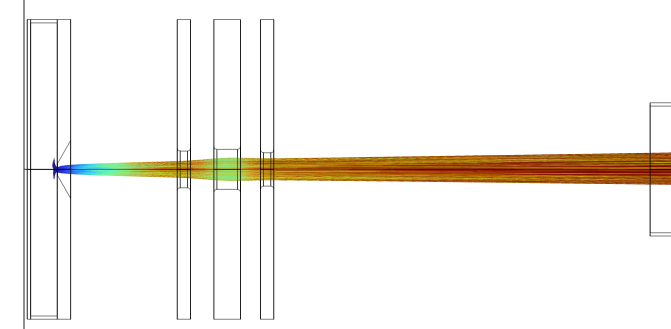
\includegraphics[width=\linewidth]{3 - COMSOL/balidazioak-ibilbideak.png}
        \caption{COMSOL-en.}
        \label{fig:comsol_trajectories_validation}
    \end{subfigure}
    \hspace{0.02\textwidth}
    \begin{subfigure}[b]{0.45\textwidth}
        \centering
        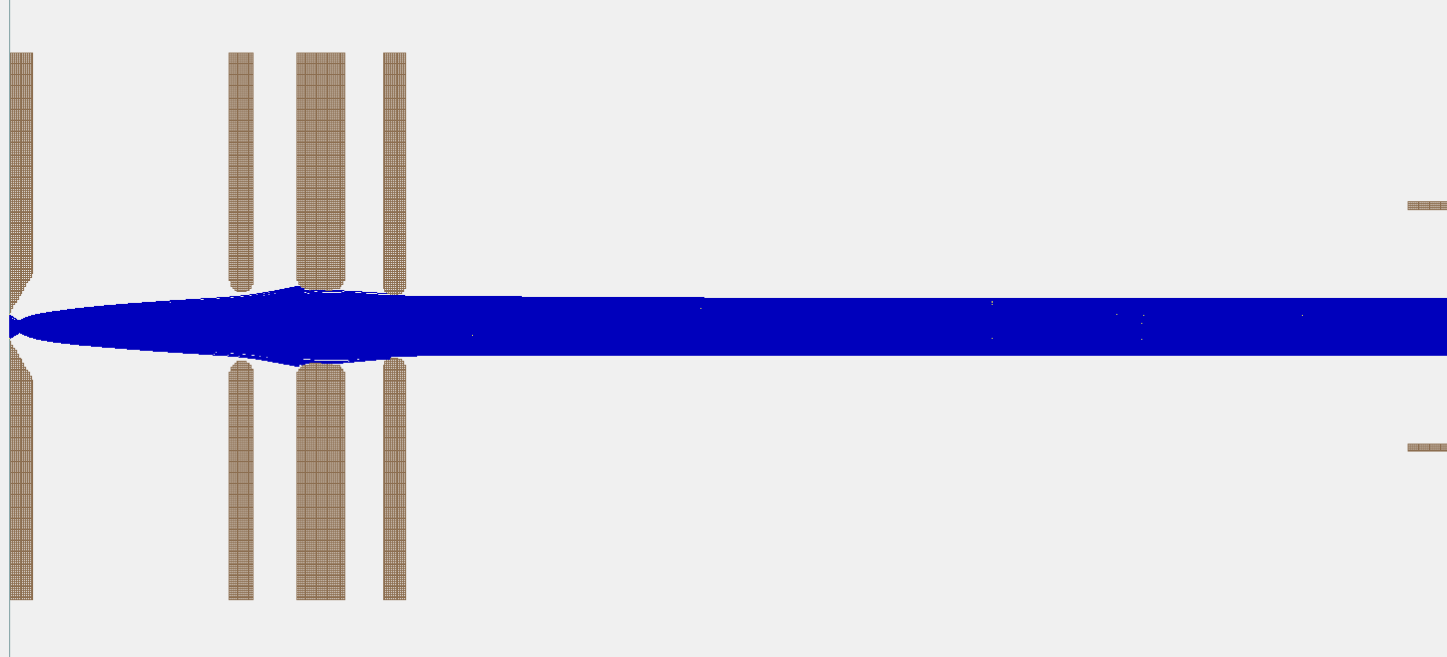
\includegraphics[width=\linewidth]{3 - COMSOL/simion_trajectories.png}
        \caption{SIMION-en.}
        \label{fig:simion_trajectory}
    \end{subfigure}
    \caption{Erauzketa-sistemaren partikulen ibilbideen simulazioen konparaketa.}
    \label{fig:partikula_ibilbideak}
\end{figure}

\begin{figure}[h]
    \centering
    \begin{subfigure}[b]{\textwidth}
        \centering
        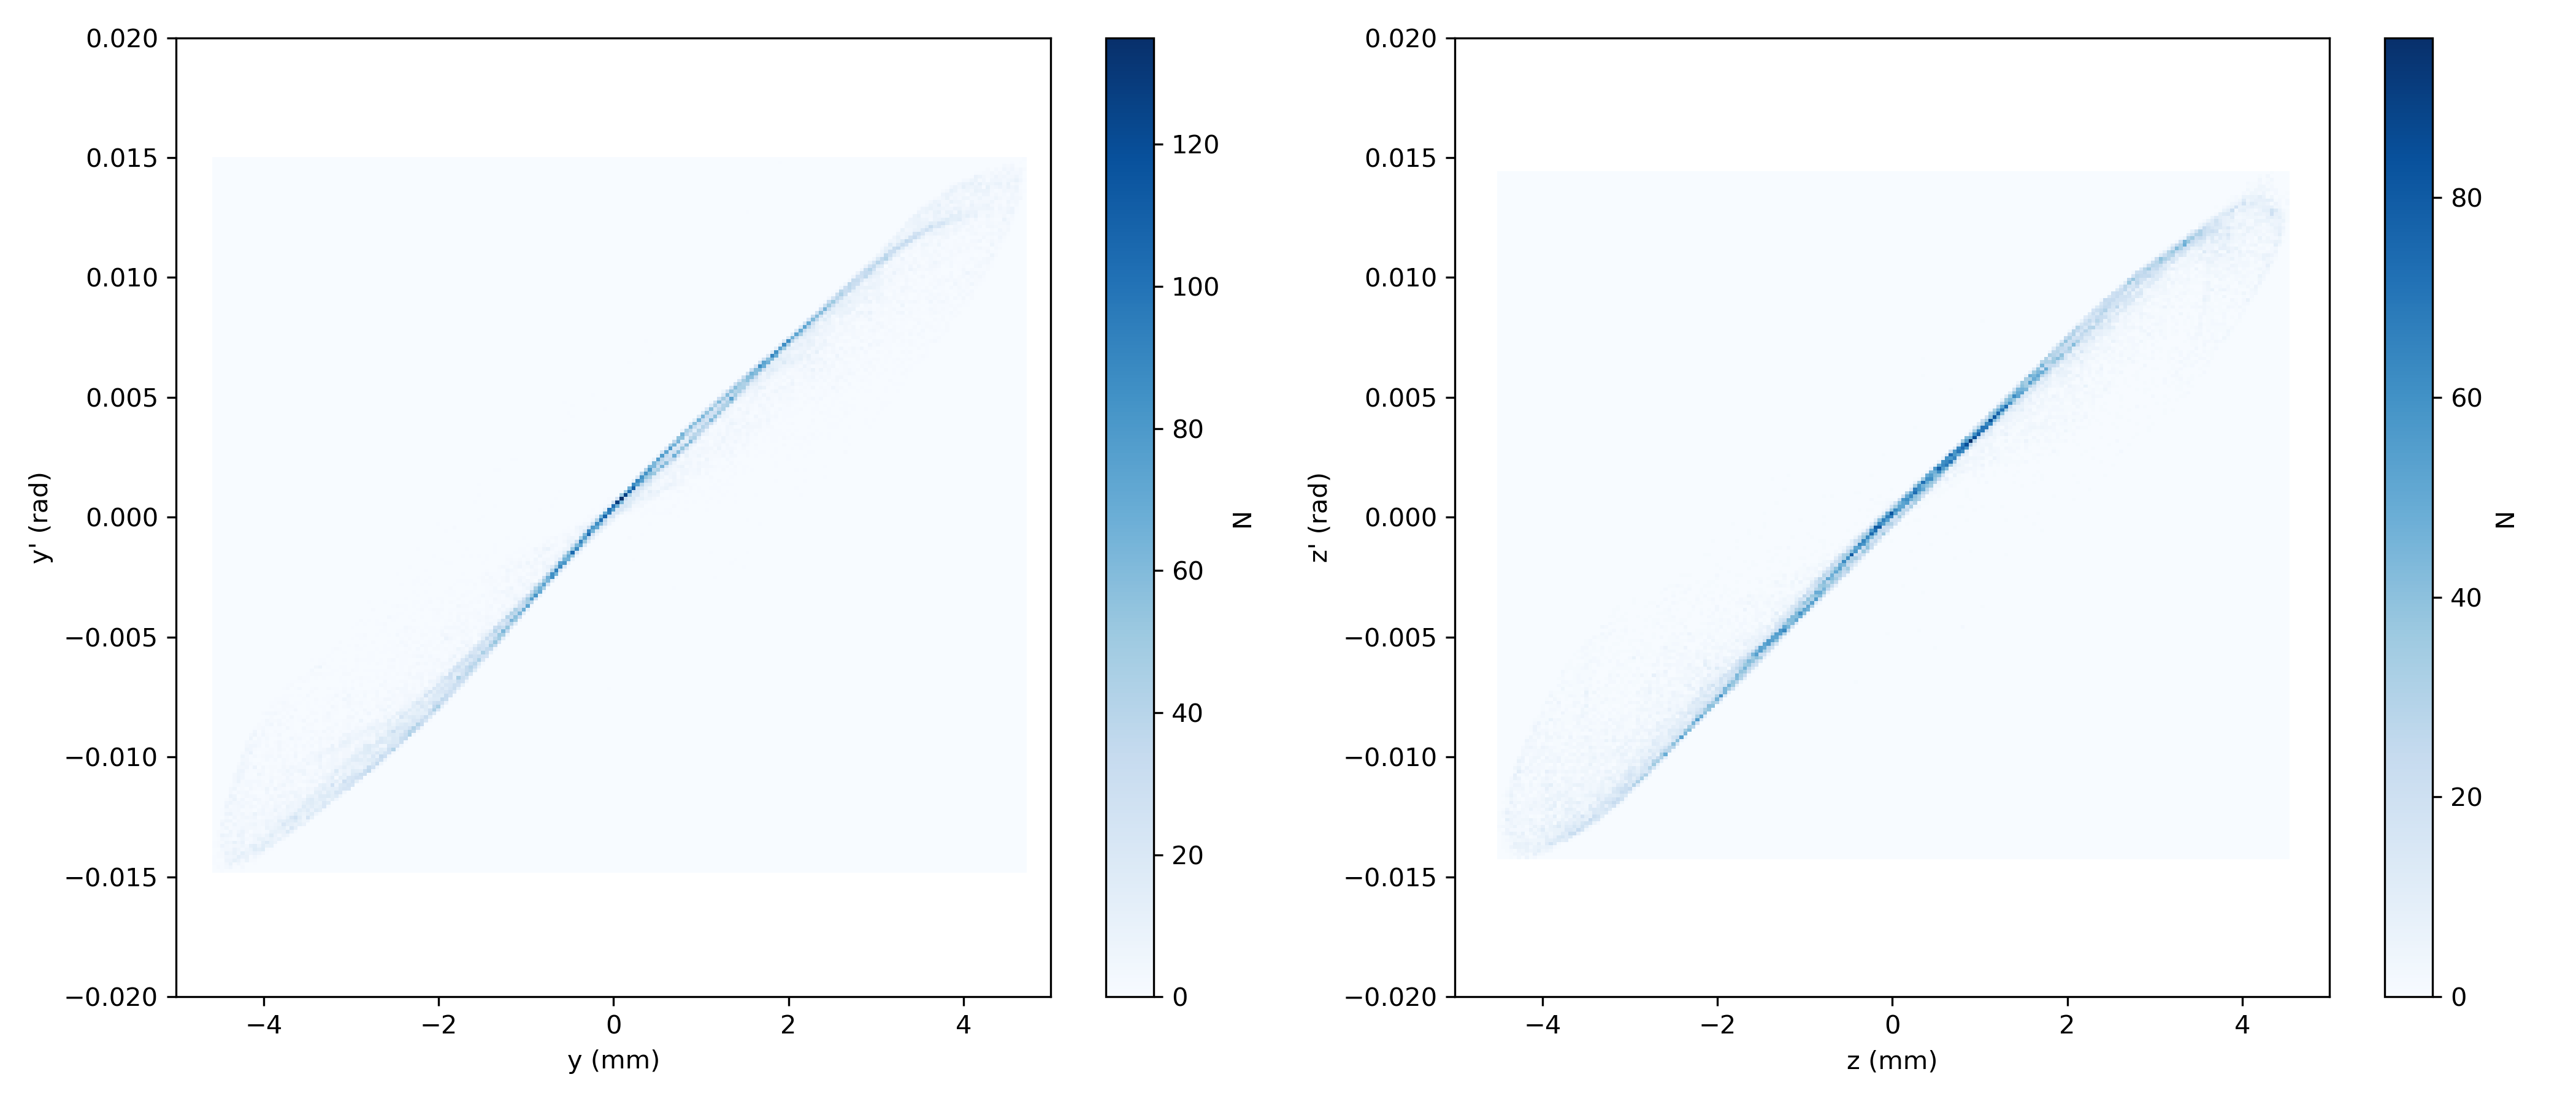
\includegraphics[width=0.8\linewidth]{3 - COMSOL/irteera_emitantziak.png}
        \caption{COMSOL-en.}
        \label{fig:comsol_emittance_valid}
    \end{subfigure}
    \vspace{0.2cm}
    \begin{subfigure}[b]{\textwidth}
        \centering
        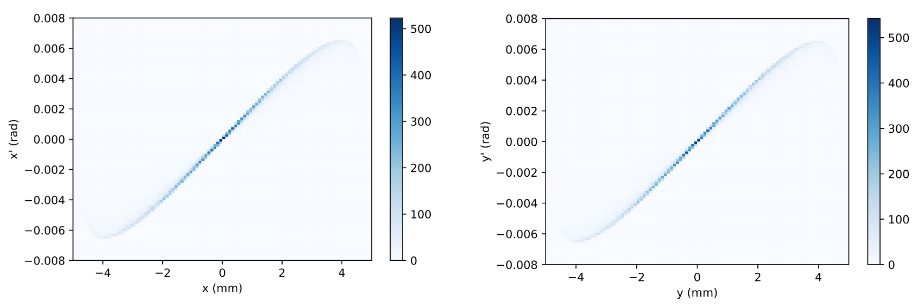
\includegraphics[width=0.97\linewidth]{3 - COMSOL/simion_emittances.png}
        \caption{SIMION-en.}
        \label{fig:simion_emittance}
    \end{subfigure}
    \caption{Ioi-izpiaren emitantziak LEBT-aren hodiaren sarreran ($x=187\;mm$).}
    \label{fig:emitantziak_valid}
\end{figure}
\newpage
\begin{table}[h]
    \centering
    \caption{LEBT-aren sarreran lortutako emitantziak ($mm\;mrad$) eta erroreak.}
    \begin{tabular}{ccc}
        \rowcolor{gray!20}
        \toprule
         & \textbf{$\epsilon_{yy',\mathrm{rms}}$} & \textbf{ $\epsilon_{zz',\mathrm{rms}}$}\\
        \specialrule{0.5pt}{0pt}{5pt} 
        COMSOL & $\num{2.508}$ & $\num{2.651}$ \\
        SIMION & $\num{2.585}$ & $\num{2.639}$\\
        \specialrule{0.5pt}{5pt}{5pt}
        Errorea & $\% \num{2.98}$ & $\% \num{0.45}$ \\
        \specialrule{1pt}{5pt}{0pt}
    \end{tabular}
    \label{tab:validation_emittances}
\end{table}

\begin{figure}[h]
    \centering
    \begin{subfigure}[b]{\textwidth}
        \centering
        \includegraphics[width=0.45\linewidth]{3 - COMSOL/exit_profile.png}
        \caption{COMSOL-en.}
        \label{fig:comsol_profile_valid}
    \end{subfigure}
    \begin{subfigure}[b]{\textwidth}
        \centering
        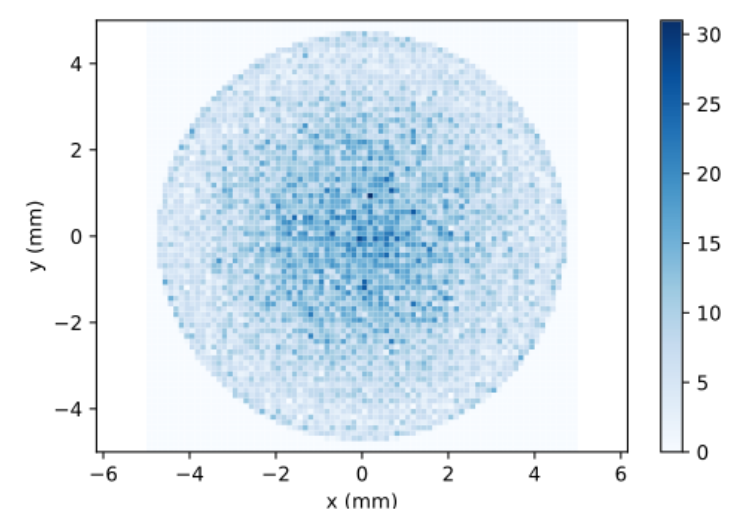
\includegraphics[width=0.45\linewidth]{3 - COMSOL/simion_profile.png}
        \caption{SIMION-en.}
        \label{fig:simion_profile}
    \end{subfigure}
    \caption{Ioi-izpiaren profila LEBT-aren hodiaren sarreran ($x=187\;mm$).}
    \label{fig:partikula_profilak_valid}
\end{figure}

Bi programetan lortutako emitantzien balioak oso antzekoak dira (\ref{tab:validation_emittances}. taula); aztarna-espazioak (\ref{fig:emitantziak_valid}. irudia) eta profilak (\ref{fig:partikula_profilak_valid}. irudia) bateragarriak dira ere, nahiz eta COMSOL-en partikula asko ertzetan pilatzen direla ikusten den. Beraz, emaitzen antzekotasuna kontuan hartuta, COMSOL-eko emaitzak fidagarritzat hartu dira, eta \textit{Wien Filter}-aren diseinua eta simulazioa bertan egin daiteke.

\newpage
\section{Diseinua eta simulazioak}
\label{sec:diseinusimulazio}
Linac-7 proiektuaren \textit{Wien Filter}-ean, eremu magnetikoa iman iraunkor finkoen bidez sortuko da; eremu elektrikoa, berriz, elektrodo paraleloekin sortuko denez, balioa aldatzeko aukera egongo da potentzialak zehaztuz, hainbat espezie aukeratzea ahalbidetuz.\\

Orokorrean, mota honetako dispositiboak Einzel lentearen ondoren instalatzen dira \cite{asaji_development_2019, storey_filtering_2024}, LEBT-an parte hartzen duten solenoideen korronteak espeziearen arabera doitzeko. Kasu honetan, LEBT-a aurretik diseinatu eta eraiki zenez, Einzel lentearekin akoplatuta dago, eta iragazkia inplementatzeko dimentsioak murriztuak dira: bi etapen arteko konexio-moduluan eraikitzea erabaki da, $118\;mm$ luzerako espazio librea dagoelako; espazio guztia ez hartzeko, ordea, $\mathbf{L=100\;mm}$-ko luzera zehaztuko da. Einzel lentearen irteeratik konexio-modulura $\num{5.8}\;mm$ daudenez, dispositiboa $12 mm$-tara ezarriko da distantzia uzteko, eta horrela iragazkiaren irteera LEBT-etik $\num{99}$ mm-ra egongo da.\\

\begin{figure}[h]
    \centering
    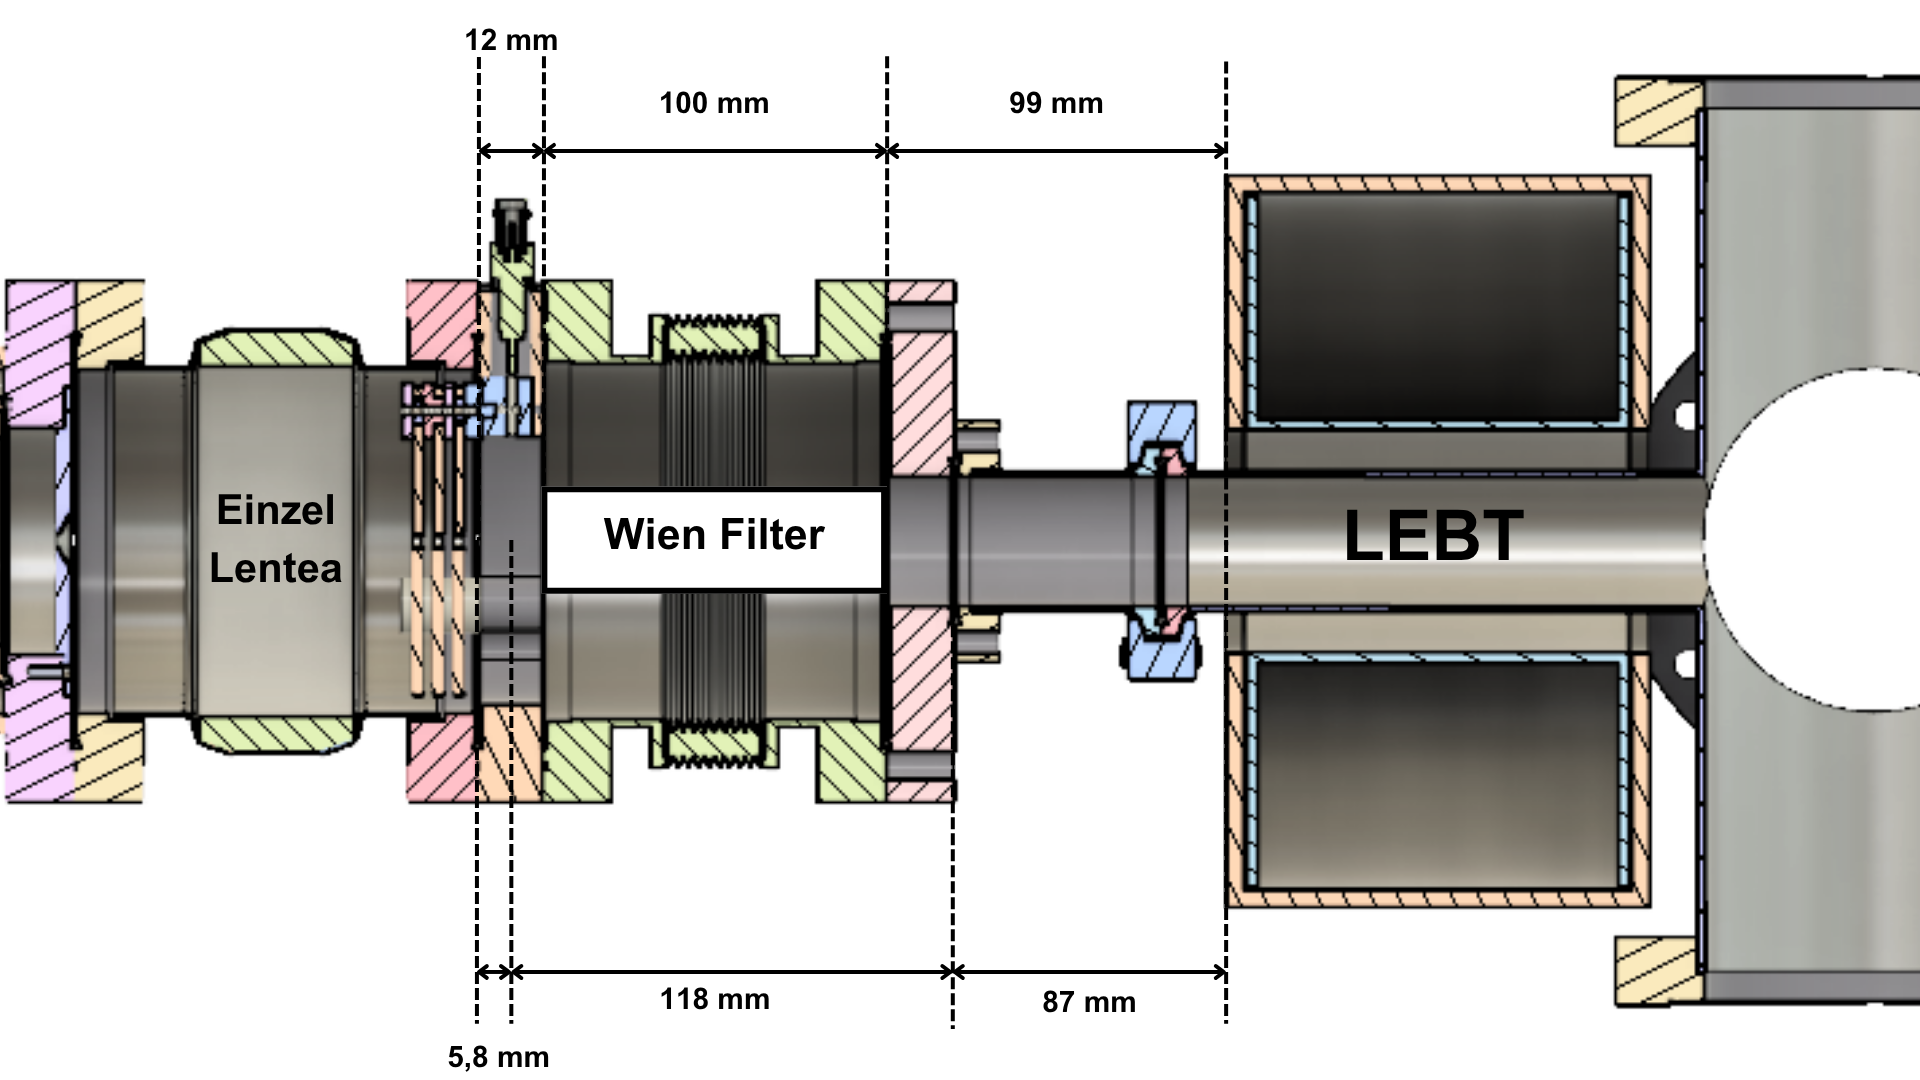
\includegraphics[width=\linewidth]{4 - Diseinua/wien_filter_position.png}
    \caption{}
    \label{fig:wien_position}
\end{figure}

Bestalde, sarrera eta irteerako zuloen erradioak zehazteko, sistemaren balidazioan lortutako izpiaren erradioak kontuan hartu dira. Profilei erreparatuz (\ref{fig:profilak} irudia), $\mathbf{r_{in}=3,5\;mm}$ aukeratu da sarreran izpi osoa sartzeko. Irteeran, ordea, izpia kolimatuko da: ertzetako partikulek Wien baldintza guztiz betetzen ez dutenez, apur bat desbideratzen dira, eta horiek baztertzea komenigarria da emitantzia hobetzeko \cite{zhang_beam_2012}. Beraz, $\mathbf{r_{out}=2,5\;mm}$ hartu da. Era berean, diseinurako simulazioen koste konputazionala murrizteko, sistema osoa simulatu ordez, iragazkiaren sarreran profil honen ezaugarriak dituen izpi bat definituko da.
\newpage

\begin{figure}[h]
    \centering
    \begin{subfigure}[b]{0.48\textwidth}
        \centering
        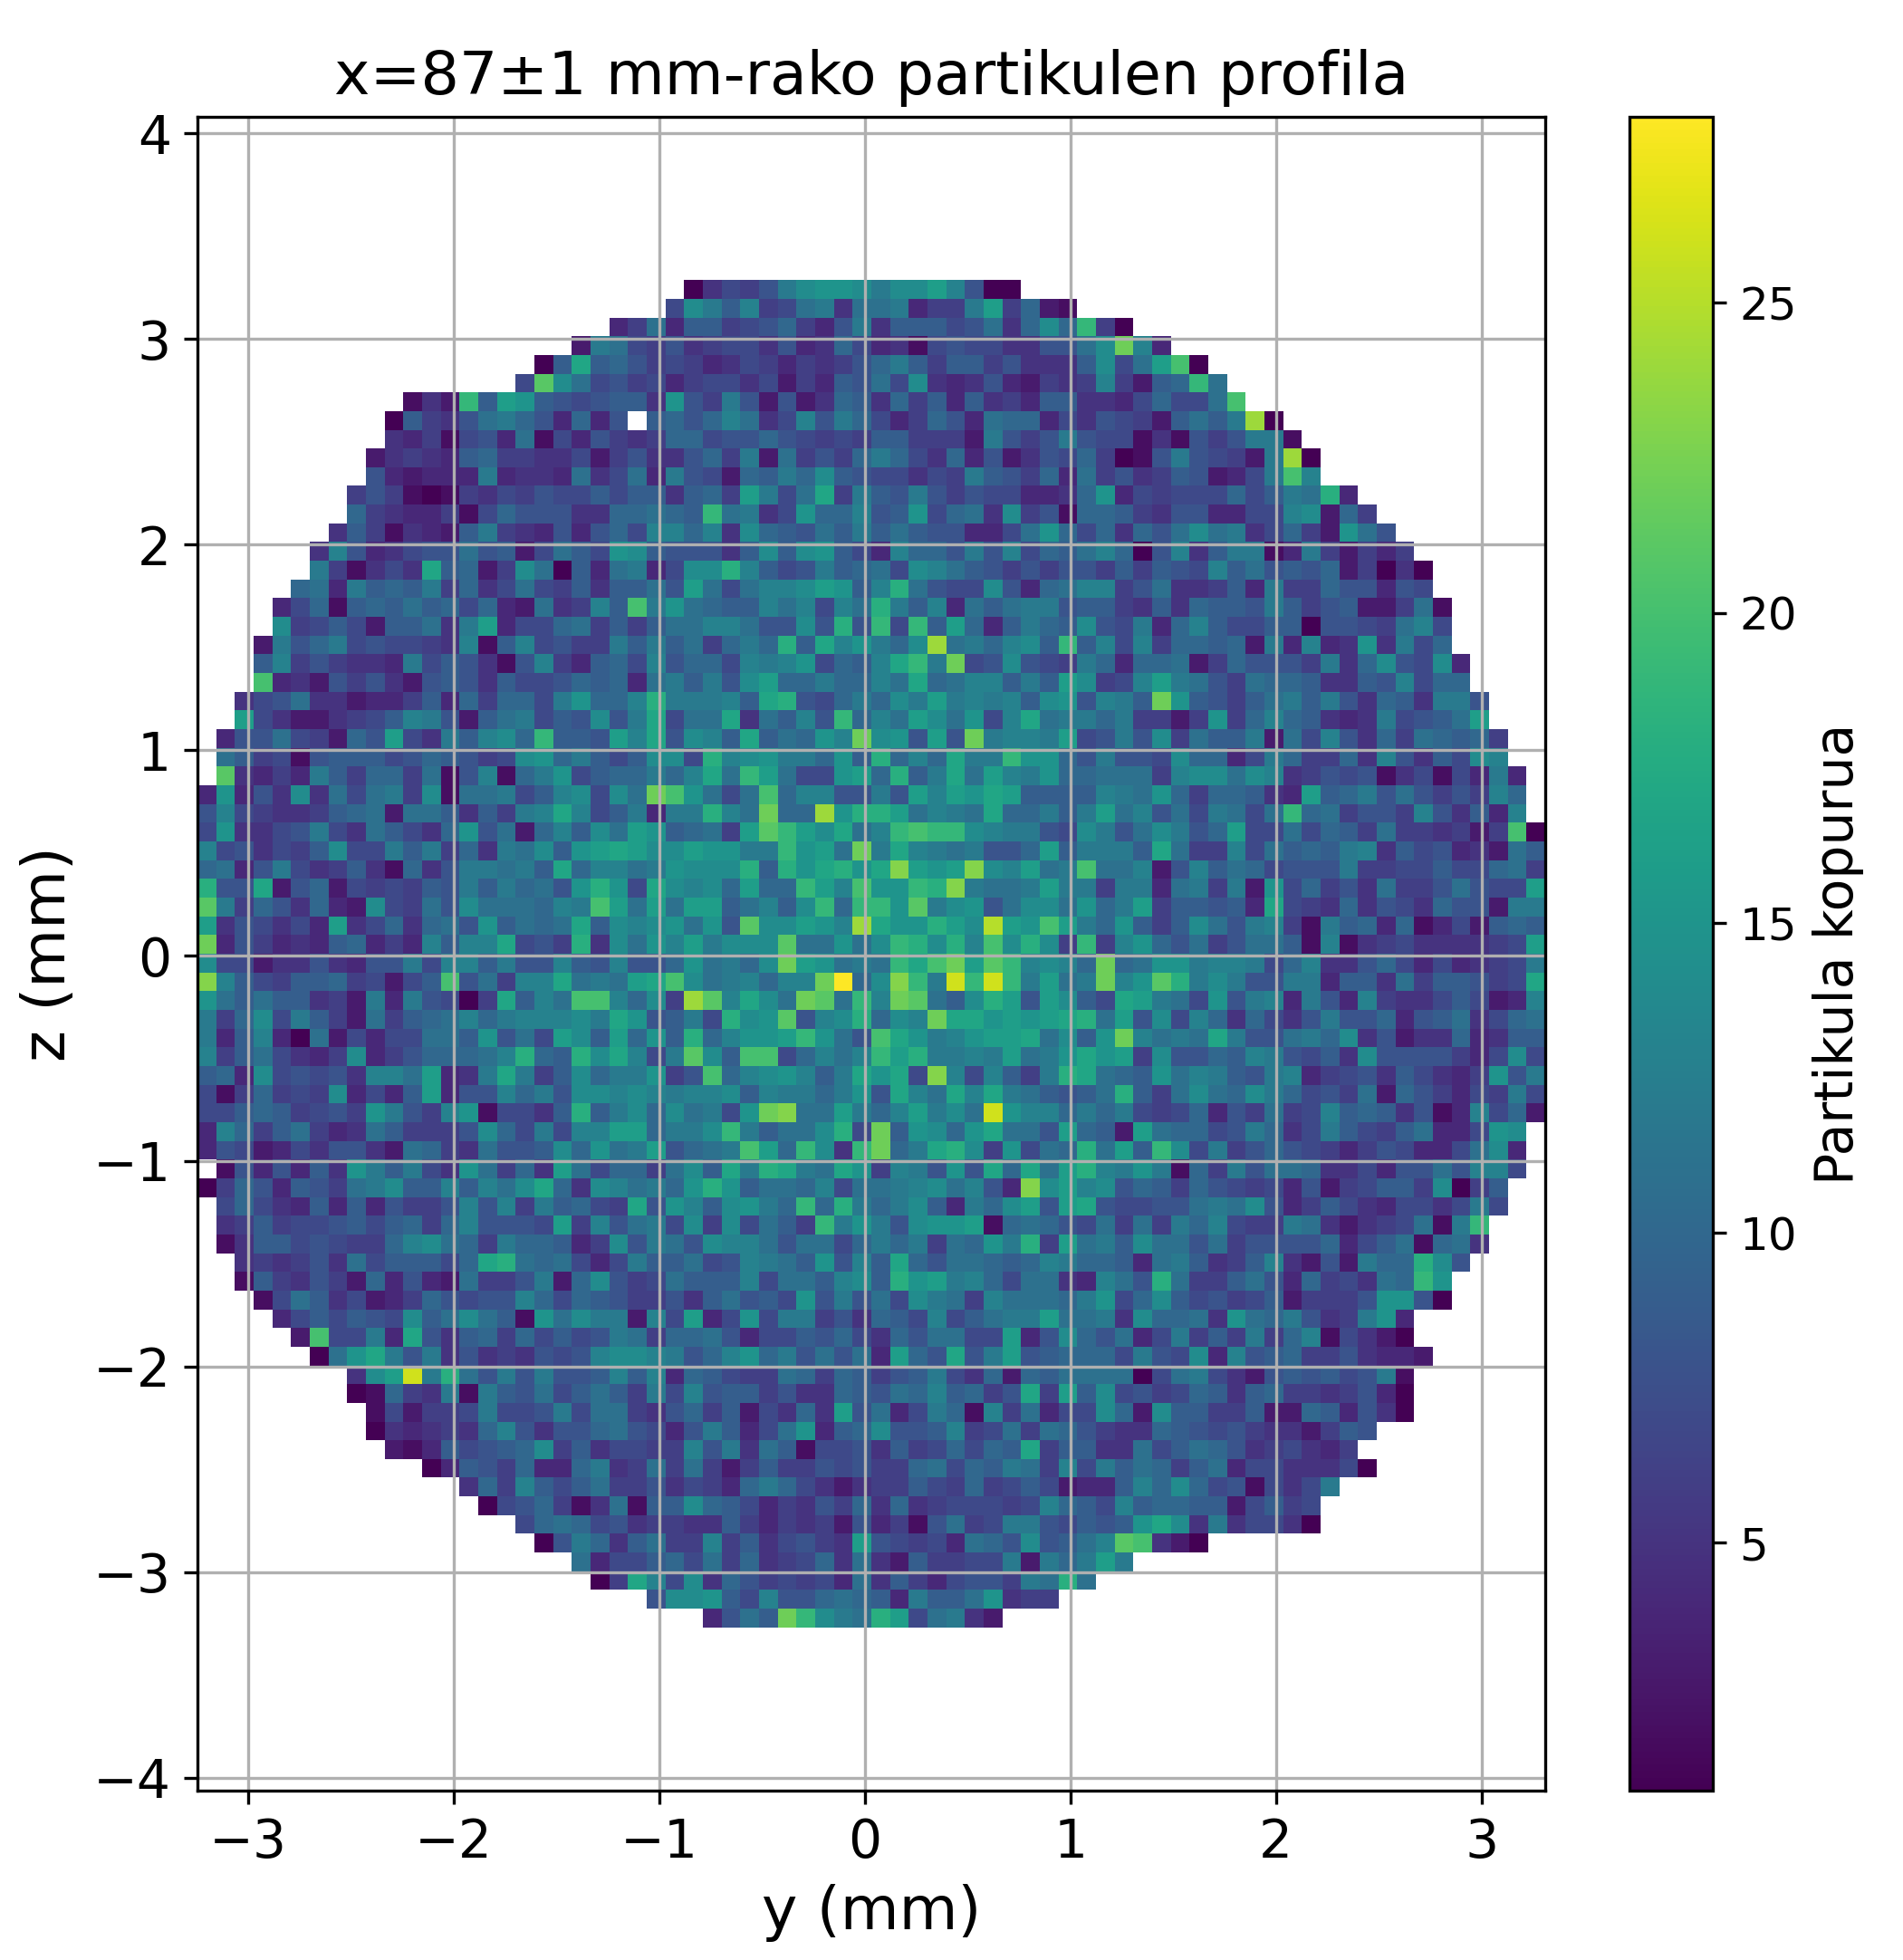
\includegraphics[width=\linewidth]{4 - Diseinua/enter_profile.png}
        \caption{Einzel lentetik $12\;mm$-ra (sarrera).}
        \label{fig:sarrera_profila}
    \end{subfigure}
    \hspace{0.01\textwidth}
    \begin{subfigure}[b]{0.48\textwidth}
        \centering
        \includegraphics[width=\linewidth]{4 - Diseinua/exit_profile.png}
        \caption{Einzel lentetik $112\;mm$-ra (irteera).}
        \label{fig:irteera_profila}
    \end{subfigure}
    \caption{Ioi-izpiaren profilak.}
    \label{fig:profilak}
\end{figure}

Hori kontuan hartuta, eremu magnetikoaren \textbf{balio minimoa finkatuko} da. Partikula baten abiadura hautatuz besteak guztiz desbideratzeko eremu magnetikoa, \ref{eq:desbiderapena} ekuazioaz kalkulatuz, \ref{tab:desbideraketa_eremuak}. taulan agertzen da, espezie bakoitzerako.\\ 

\begin{table}[h]
    \centering
    \caption{Espezie desberdinak guztiz desbideratzeko eremu minimoak.}
    \begin{tabular}{c|c|c|c}
         \rowcolor{gray!20}
         \toprule
         &$\mathbf{H^+}$ \textbf{aukeratzeko} & $\mathbf{H_2^+}$ \textbf{aukeratzeko} & $\mathbf{H_3^+}$ \textbf{aukeratzeko} \\
         \midrule 
         $\mathbf{H^+}$ \textbf{desbideratzeko} & & B = \num{102.5}\;mT & B=71\;mT\\
         \midrule
         $\mathbf{H_2^+}$ \textbf{desbideratzeko} & B = \num{102.5}\;mT  & & B = \num{231.5}\;mT \\
         \midrule
         $\mathbf{H_3^+}$ \textbf{desbideratzeko} & B=71\;mT & B = \num{231.5}\;mT & \\
        \bottomrule
    \end{tabular}
    \label{tab:desbideraketa_eremuak}
\end{table}

Kalkulatutako eremuak minimoak direnez, espezie guztien desbiderapena ziurtatzeko handiena hartuko da: $\mathbf{B_{min}=231,5\;mT}$. Garrantzitsua da eremu magnetikoa ahalik eta txikiena izatea, ezarriko den eremu elektrikoa horren proportzionala denez, elektrodoen potentzialak ere proportzionalak direlako, eta segurtasunerako tentsio baxuak ezartzea komenigarria da: $\mathbf{\pm4kV}$-etara mugatuko dira. Dena dela, iman iraunkorretarako balio zehatzak lortzea oso zaila denez, $B_{min}$ soilik behe-mugatzat hartuko da.

\subsection{Lehenengo diseinua eta mugaketak}

Lehenengo diseinurako, \ref{sec:elektrodo_paraleloak} eta \ref{sec:iman_iraunkorrak} ataletan landutako egitura idealak zuzenean simulatuko dira: elektrodo lau paraleloak eta aurrez-aurreko iman iraunkorrak, bien luzera dispositibo osoarena izanik, $L=100\;mm$ (\ref{fig:wien_ideal}. irudia). 
\newpage
\begin{figure}[h]
    \centering
    \begin{subfigure}[b]{0.45\textwidth}
        \centering
        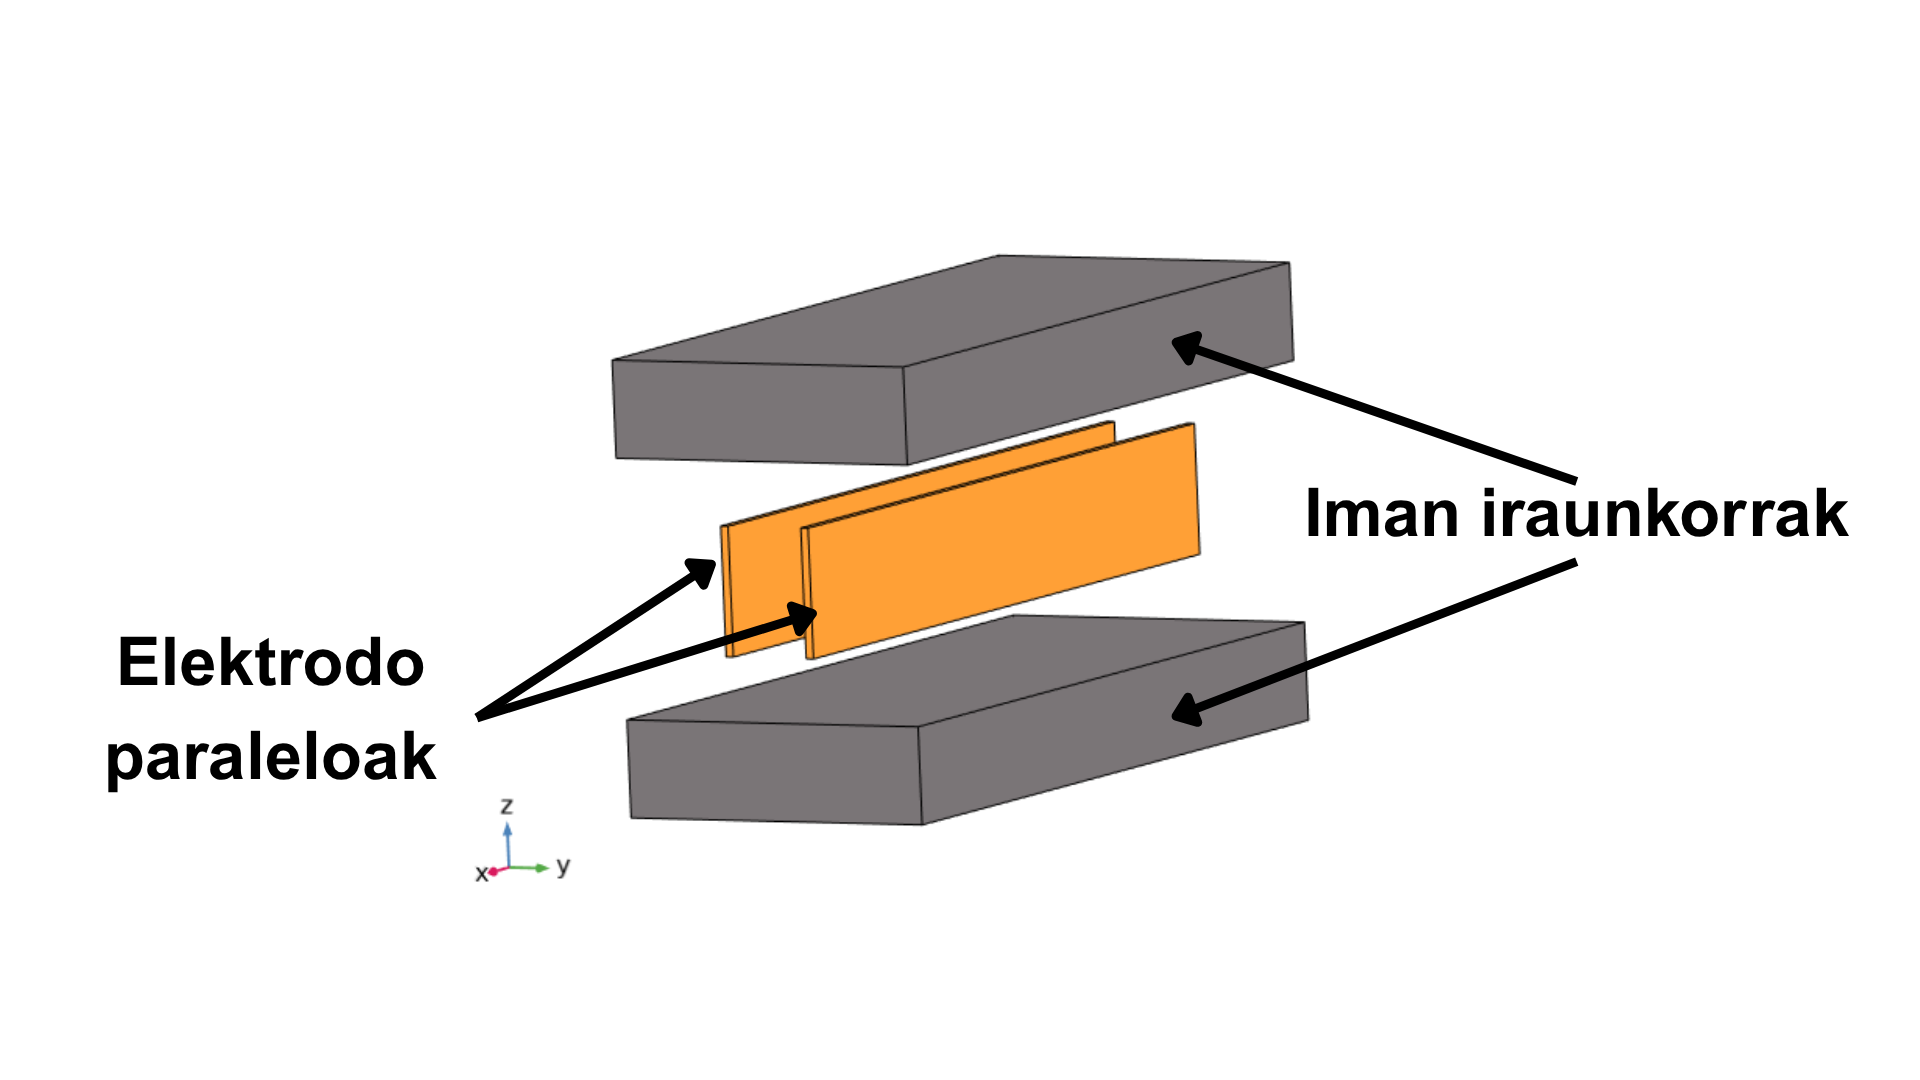
\includegraphics[width=\linewidth]{4 - Diseinua/wien_filter_ideal1.png}
        \caption{Ikuspegi orokorra 3D-n.}
        \label{fig:wien_ideal_1}
    \end{subfigure}
    \hspace{0.02\textwidth}
    \begin{subfigure}[b]{0.45\textwidth}
        \centering
        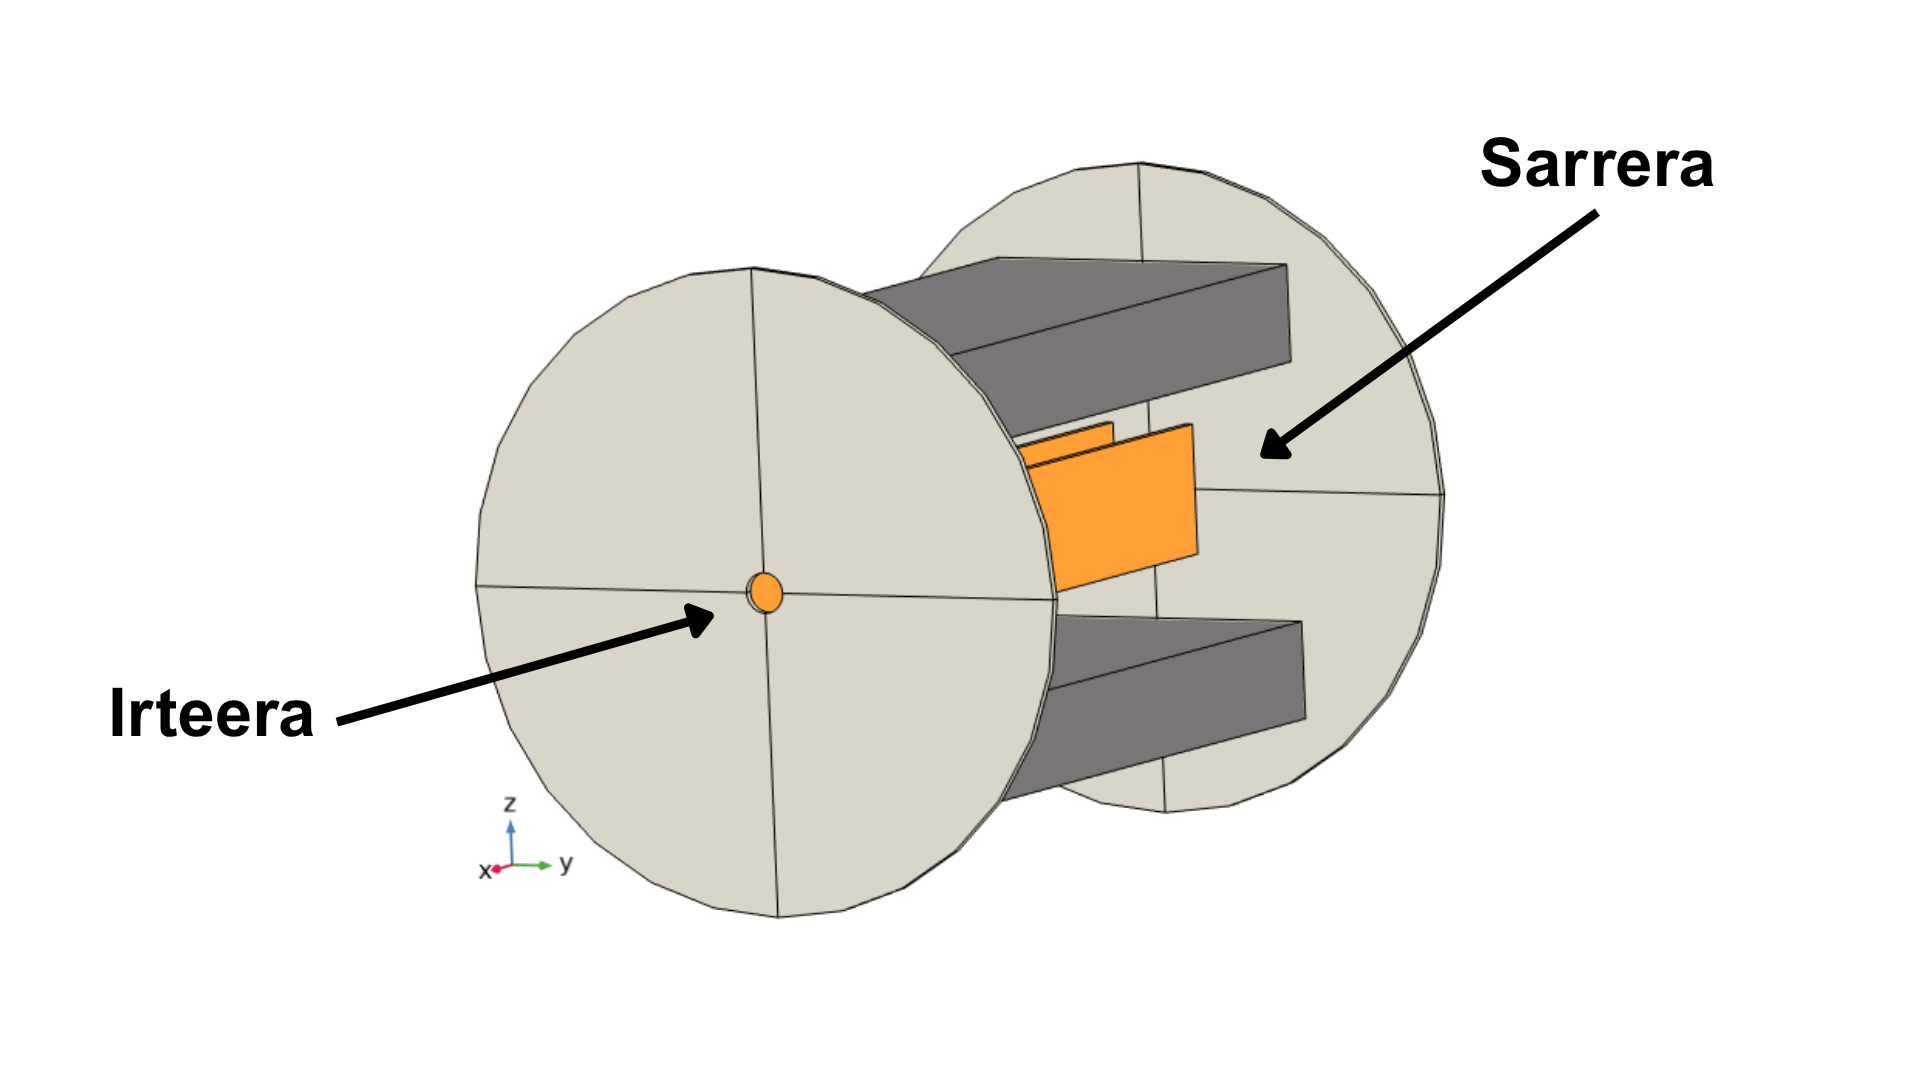
\includegraphics[width=\linewidth]{4 - Diseinua/wien_filter_ideal2.png}
        \caption{yz planoaren eskema.}
        \label{fig:wien_ideal_2}
    \end{subfigure}
    \caption{\textit{Wien Filter}-aren lehenengo diseinua COMSOL-en.}
    \label{fig:wien_ideal}
\end{figure}

Imanen kasuan, \textbf{NdFeB materiala} aukeratu da, N52 hain zuzen ere, indukzio magnetiko erremanente handia eskaintzen duelako ($B_{r,N52}\simeq \num{1.44}\;T$) prezio nahiko baxurako. \textit{Supermagnete}-n, adibidez, N52-ko $10\times10\times\num{1.2}\;mm$-ko blokeak $\num{0.51}$€/unitate-ra saltzen dira hamarnaka \cite{ag_bloque_nodate}, eta horiek hartuko dira erreferentziatzat diseinurako. Bi blokeen artean neurtutako eremua \ref{fig:bloke_magnetiko} ekuazioaz kalkulatu daiteke $B=2\cdot B_{bloke}(d_m/2)$ hartuz. Kalkuluen eta simulazioen emaitzak \ref{tab:eremumag_balio}. taulan ikusi daiteke, hainbat iman batera erabiliz.\\

\begin{table}[h]
    \centering
    \caption{Eremu magnetikoen kalkuluen eta simulazioen balioak.}
    \begin{tabular}{cc}
        \textbf{Iman luzera:} & $\mathbf{L=100\;mm}$ (10 iman)\\
        \textbf{Iman zabalera:} & $\mathbf{W=40\;mm}$ (4 iman)\\
        \textbf{Iman altuera:} & $\mathbf{D=12\;mm}$ (10 iman)\\
        \textbf{Iman arteko distantzia:} & $\mathbf{d_m=32\;mm}$ \\
        \midrule
        \rowcolor{gray!20}
        $\mathbf{B_{kalkulu}}$ & $\mathbf{B_{simulazio}}$\\
        \midrule
        $262\;mT$ & $265\;mT$\\
        \bottomrule
    \end{tabular}
    \label{tab:eremumag_balio}
\end{table}

Eremu magnetikoa izanda, espezie desberdinak aukeratzeko potentzialak kalkulatu ditzakegu elektrodoen arteko distantzia zehaztuz. Txikia izatea komenigarria da potentzialak ahalik eta txikienak izateko, baina haustura-tentsioa distantziaren araberakoa dela kontuan hartu behar da. Orduan, izpi osoa igaro dadin, $\mathbf{d_e=10\;mm}$ aukeratu da. \ref{tab:eremue_balio}. taulan ikusi daitezke \ref{eq:eremue_paralelo} ekuazioaz eta simulazioen bidez lortutako balioak.\\

\begin{table}[h]
    \centering
    \caption{Wien baldintza betetzeko eremu elektrikoak eta potentzialak.}
    \begin{tabular}{cccc}
        & \textbf{Elektrodo luzera:} & $\mathbf{L=100\;mm}$ &\\
        & \textbf{Elektrodo zabalera:} & $\mathbf{W=16\;mm}$ &\\
        & \textbf{Elektrodo altuera:} & $\mathbf{D=1\;mm}$ &\\
        & \textbf{Elektrodo arteko distantzia:} & $\mathbf{d_e=10\;mm}$ &\\
        \midrule
        \rowcolor{gray!20}
        & $\mathbf{E_{kalkulu}}$ (kV/m) & $\mathbf{V_{\pm}}$ (V)&$\mathbf{E_{simulazio}}$ (kV/m)\\
        \midrule
        $\mathbf{H^+}$ \textbf{aukeratzeko} & $\num{635.36}$ & 3177 & $\num{632.68}$\\
        $\mathbf{H_2^+}$ \textbf{aukeratzeko} & $\num{449.18}$  & 2246 & $\num{447.63}$\\
        $\mathbf{H_3^+}$ \textbf{aukeratzeko} & $\num{366.76}$ & 1834 & $\num{365.52}$\\
        \bottomrule
    \end{tabular}
    \label{tab:eremue_balio}
\end{table}

Eremuetarako simulazioak kalkulatutako balioekin bat datoz. Partikulen ibilbideak simulatzerakoan, ordea, ez da esperotakoa lortzen: hautatutakoak ez diren espezieak iragaztea lortzen da, baina izpi-nagusiak ere desbiderapena jasaten du, sistemaren portaera idealetik aldentzen dela azaleratuz. Erantzuna \textbf{ertz-eremuetan} (\textit{fringing fields}) aurkitu daiteke.

\begin{figure}[h]
    \centering
    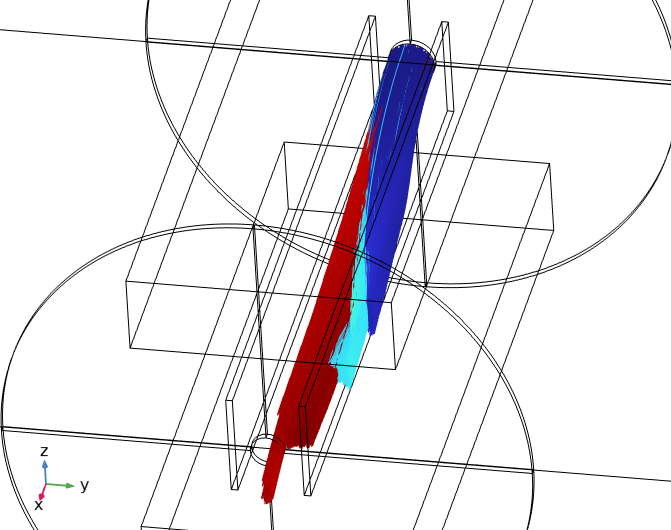
\includegraphics[width=0.6\linewidth]{4 - Diseinua/partikulak_ideal1.png}
    \caption{Partikulen ibilbideak, $B=265\;mT$, $V_\pm=3177\;V$ izanik (\colorbox{red}{$\mathbf{H_{ }^+}$}, \colorbox{cyan}{$\mathbf{H_2^+}$}, \colorbox{blue}{$\mathbf{H_3^+}$}).}
    \label{fig:partikulak_ideal1}
\end{figure}

Alde batetik, izpiaren hedatze-ardatzerako eremu elektriko eta magnetikoaren gainezarmenari erreparatuz gero (\ref{fig:eremu_gainezarmena_1}. irudia), erdialdeko zonaldean bat datozela eta konstanteak direla ikusi daiteke, baina sarrerako eta irteerako zonaldeetan, ordea, eremu elektrikoak gradiente espazial handiago du. Eremuen arteko desfaseak Wien baldintza ez betetzea eragiten du, iragazkiaren eraginkortasuna kaltetuz.

\begin{figure}[h]
    \centering
    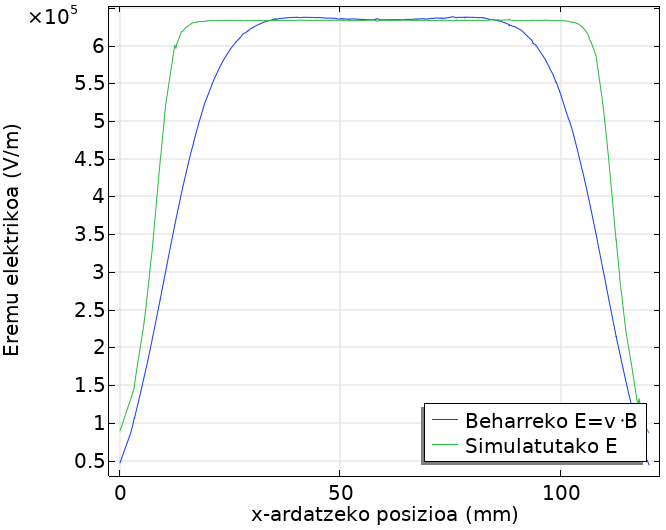
\includegraphics[width=0.6\linewidth]{4 - Diseinua/eremu_gainezarmena_1.png}
    \caption{Eremu elektriko eta magnetikoen gainezarmena ($E_f=B\cdot v_f$) $x$-ardatzean.}
    \label{fig:eremu_gainezarmena_1}
\end{figure}
\newpage

Bestetik, $y$-ardatzeko eremu magnetikoari dagokionez (\ref{fig:eremu_magnetikoa_1}. irudia), ertzetako balioa erdialdekoa baino txikiagoa dela ikus daiteke; izan ere, blokeen arteko distantziaren ondorioz, ertzetako eremu-lerroak kurbatzen dira, eremu magnetikoaren intentsitatea txikituz. Desoreka horrek iragazkiaren eraginkortasuna nabarmen kaltetzen du ere.

\begin{figure}[h]
    \centering
    \begin{subfigure}[b]{0.45\textwidth}
        \centering
        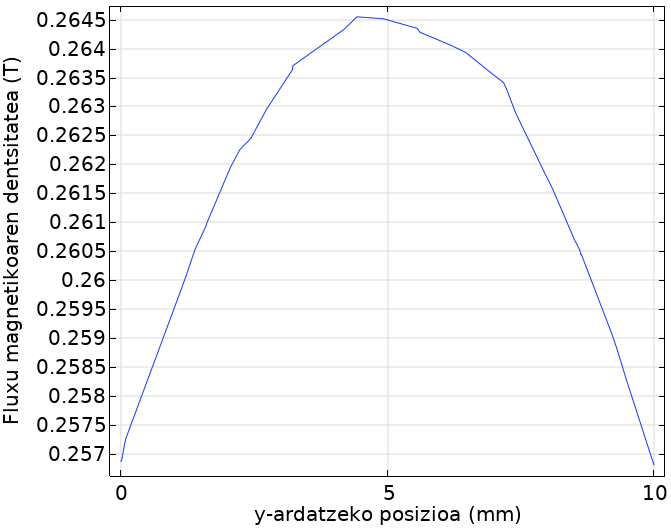
\includegraphics[width=\linewidth]{4 - Diseinua/eremu_magnetikoa_z1.png}
        \caption{Eremu-intentsitatea $y$-ardatzean.}
        \label{fig:eremu_magz_1}
    \end{subfigure}
    \hspace{0.02\textwidth}
    \begin{subfigure}[b]{0.45\textwidth}
        \centering
        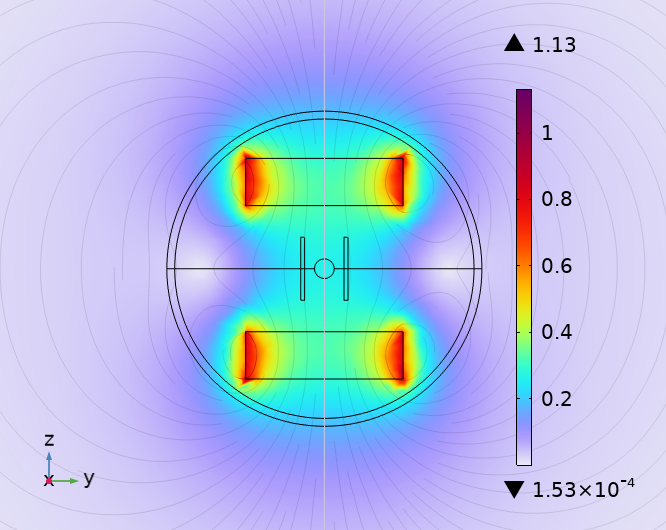
\includegraphics[width=\linewidth]{4 - Diseinua/eremu_magnetikoa_1.png}
        \caption{Fluxu-lerroen kurbatzea eta pilaketa.}
        \label{fig:fluxu_lerroak_1}
    \end{subfigure}
    \caption{Iragazkiko iman iraunkorrek sortutako eremu magnetikoa.}
    \label{fig:eremu_magnetikoa_1}
\end{figure}

\subsection{Eremu doiketa eta diseinu finala}
\label{sec:diseinu-finala}
Ertz-efektuek sortutako ez-idealtasunei aurre egiteko, bi konponbide aztertuko dira: \textbf{\textit{Rogowski}-ren profilak}, eremu elektrikoaren gradiente espaziala doitzeko, eta \textbf{burdin gozozko uztarria}, eremu magnetikoaren fluxu-lerroak bideratzeko.

\subsubsection{Rogowskiren profilak}

Elektrodoen amaierako ertzetako bat-bateko gradientea zuzentzeko, konponbide intuitibo bat muturrak kurbatzea izan daiteke, eremu elektrikoaren beherakada leuntzeko. Horren antzera, plaka paraleloen lerro ekipotentzialak jarraitzen dituzten profilak erabili daitezke, \textit{Rogowski}-ren profilak deritzenak \cite{rogowski_elektrische_1923} eta \textit{Wien Filter}-etan oso erabiliak direnak \cite{palacios_serrano_high_2021}. Orekako eroaleen gainazalak ekipotentzialak direnez, profilek lerro horiek jarraituz gero, lerroek ekipotentzial izaten jarraituko dute, eskualde idealeko eremu elektrikoa ez aldatuz eta beherakada leunduz.\\

\textit{Rogowski}-k lerro ekipotentzialentzat proposatutako parametrizazioa \cite{wei_designing_2021},

\begin{equation}
    \begin{aligned}
        x &= \frac{d_e}{\pi}(\phi + e^\phi \cos \psi)\\
        y &= \frac{d_e}{\pi}(\psi + e^\phi \sin \psi)
    \end{aligned}
\end{equation}
\\
non $d_e$ elektrodoen arteko distantzia den, eta $\phi$ eta $\psi$ eremu desberdinak eta lerro ekipotentzial desberdinak diren. $\psi \in (0,\pi)$ edozein baliorako eremu uniformeko elektrodoentzako profilak lortzen direnez, $\psi=\frac{\pi}{2}$ aukeratu da, parametrizazio sinpleena ematen duelako.

\begin{figure}[h]
    \centering
    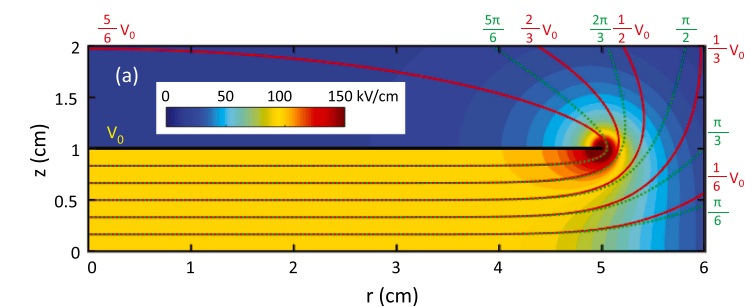
\includegraphics[width=0.75\linewidth]{4 - Diseinua/lerro_ekipotentzial.jpg}
    \caption{Elektrodo paraleloek sortutako lerro ekipotentzialak eta horien parametrizazioa \cite{wei_designing_2021}.}
    \label{fig:erro_ekipotentzial}
\end{figure}

\begin{equation}
    \begin{aligned}
        x &= \frac{d_e}{\pi}\phi\\
        y &= \frac{d_e}{\pi}(e^\phi+\frac{\pi}{2})
    \end{aligned}
    \label{eq:rogowski}
\end{equation}\\

Beraz, \ref{eq:rogowski} ekuazioko parametrizazioak COMSOL-en inplementatu dira $\phi \in (-2\pi, 0)$ hartuz, eta \ref{fig:rogowski_wien}. irudian ikus daiteke 3D-ko geometria elektrodo paraleloentzat. Elektrodoen zonalde laua profilarekin bat etortzeko doitu da.

\begin{figure}[h]
    \centering
    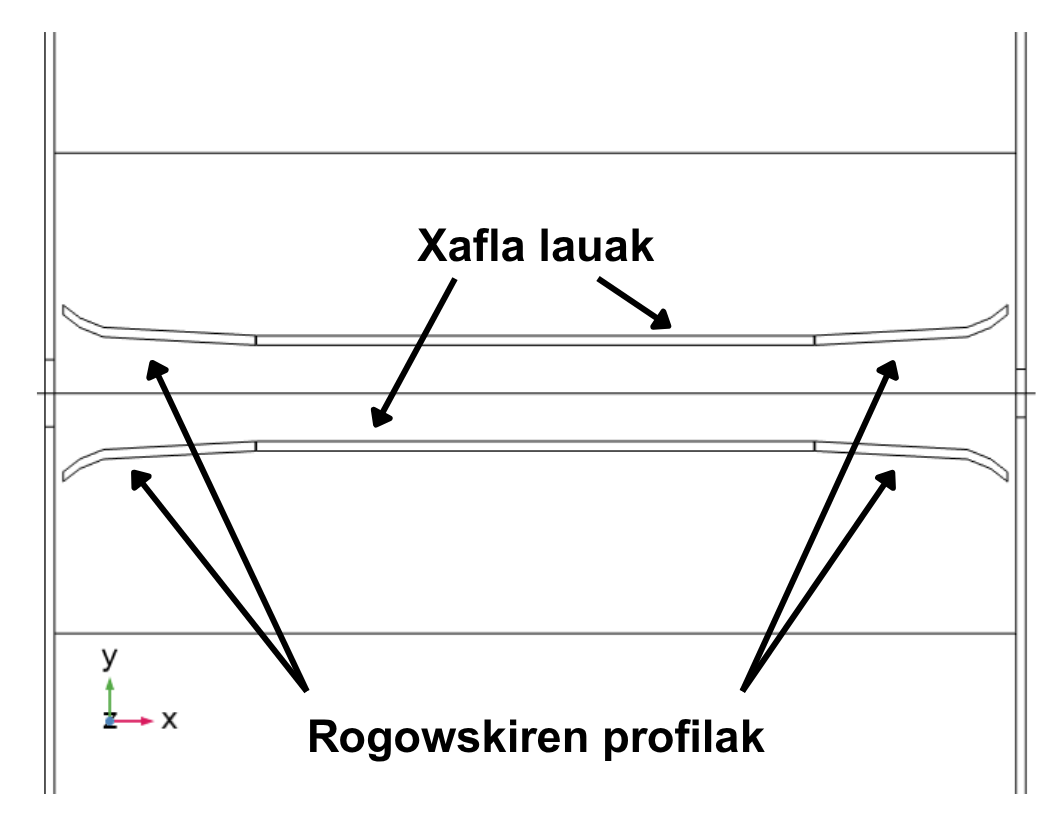
\includegraphics[width=0.6\linewidth]{4 - Diseinua/rogowski_profilak_wien.png}
    \caption{Diseinatutako \textit{Rogowski}-ren profilak, $d_e=10\;mm$ izanik.}
    \label{fig:rogowski_wien}
\end{figure}

\subsubsection{Burdin gozozko uztarria}

Eremu magnetikoaren fluxu-lerroen kurbatzea konpontzeko, ohikoa da burdin gozozko uztarriak erabiltzea \cite{peng_enhance_2023}, horren permeabilitate magnetiko handiari esker ($\mu_r\approx2000$) eremu-lerroak bertatik bideratzen baitira. Horrela, lerroak airean kurbatzea saihesten da, uniformetasuna nabarmen handituz.\\

Hala ere, material ferromagnetikoak asetu daitezke, eta uztarrien eraginkortasunean eragin handia izan dezake. Asetuz gero, fluxua ezin da uztarriaren barruan kontzentratu, eta berriro ere airera igarotzen denez, ertz-efektuak areagotuko dira. Garrantzitsua da uztarriarentzako neurri egokiak zehaztea, asetasuna zehar-sekzioaren araberakoa delako. Horrez gain, uztarriak zirkuitu magnetikoa aldatzen duenez, iman iraunkorrentzat garatutako \ref{eq:eremuuniforme} ekuazioa ez da erabilgarria, eta konfigurazioa guztiz aldatu behar da. Balioa zuzenean simulazioetatik lortuko da (\ref{tab:uztarri_magnetiko}. taula).\\

\begin{table}[h]
    \centering
    \caption{Burdin gozozko uztarriaren eta imanen neurriak, eta baita simulatutako eremu magnetikoaren balioa.}
    \begin{tabular}{cc}
        \toprule
        \textbf{Iman luzera:} & $\mathbf{L=100\;mm}$ (10 iman)\\
        \textbf{Iman zabalera:} & $\mathbf{W=60\;mm}$ (6 iman)\\
        \textbf{Iman altuera:} & $\mathbf{D=}$ \textbf{2,4 mm} (2 iman)\\
        \textbf{Iman arteko distantzia:} & $\mathbf{d_m=18\;mm}$ \\
        \midrule
        \rowcolor{gray!20}
        \multicolumn{2}{c}{$B_{simulazio}$} \\
        \midrule
        \multicolumn{2}{c}{$\num{287}\;mT$} \\
        \midrule
        \textbf{Uztarri luzera:} & $\mathbf{L_u=100\;mm}$\\
        \textbf{Uztarri zabalera:} & $\mathbf{W_u=120\;mm}$\\
        \textbf{Uztarri altuera:} & $\mathbf{D_u=}$ \textbf{32,8 mm}\\
        \textbf{Zuloaren zabalera:} & $\mathbf{w_u=}$ \textbf{110 mm} \\
        \textbf{Zuloaren altuera:} & $\mathbf{h_u=}$ \textbf{22,8 mm} \\
        \bottomrule
    \end{tabular}
    \label{tab:uztarri_magnetiko}
\end{table}
\begin{figure}[h]
    \centering
    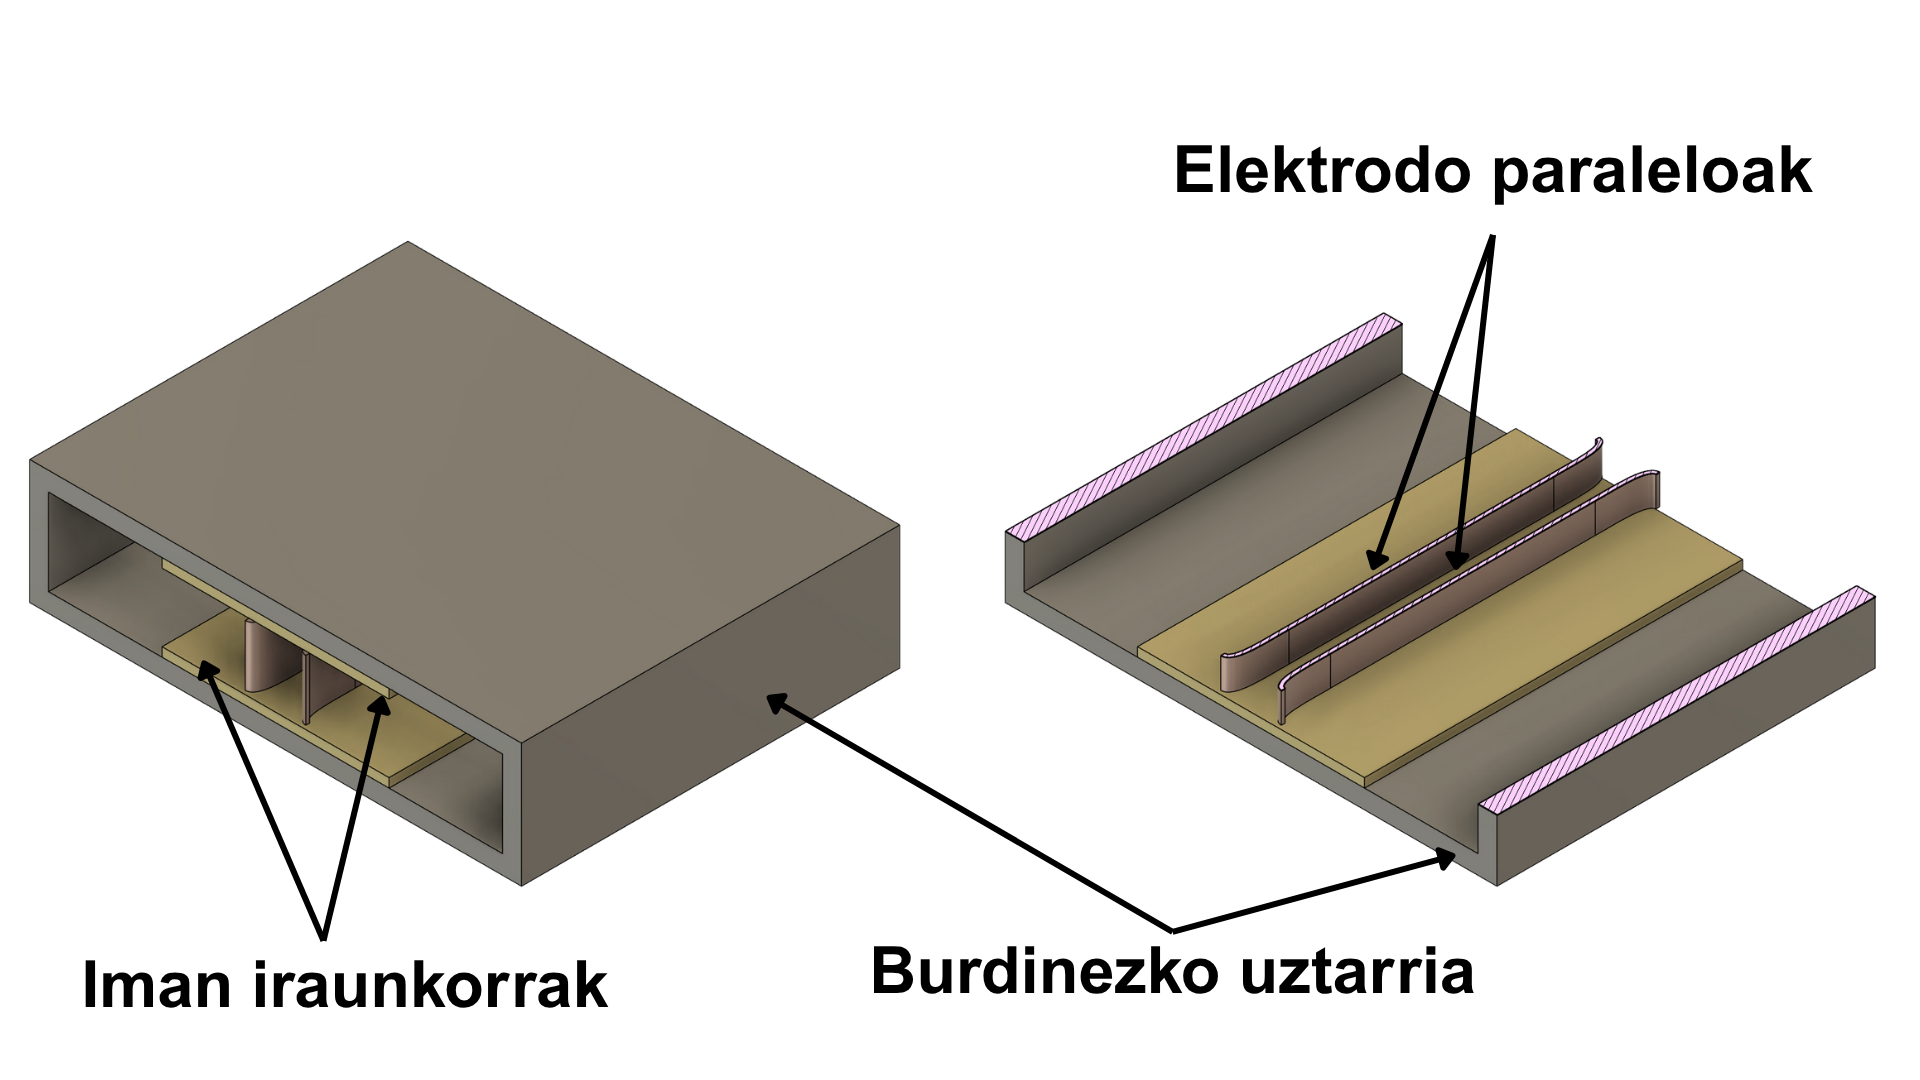
\includegraphics[width=0.9\linewidth]{4 - Diseinua/wien_filter_final1.png}
    \caption{\textit{Wien Filter}-aren diseinu finala 3D-n.}
    \label{fig:wien_final_1}
\end{figure}

\ref{fig:wien_final_1}. irudian ikus daitekeenez, uztarriak imanen arteko eremu magnetikoaren intentsitatea asko handitzen du, eta aurreko konfigurazioaren balio antzekoak lortzeko bi iman baino ez dira behar magnetizazioaren norabidean, imanen kostua murriztuz ere.\\

 Gainera, $y$-ardatzeko eremua askoz uniformeagoa da: lehen aldaketa $\% \num{3}$-koa zen, eta orain $\%\num{0.03}$-koa, espezifikazioak hobeto betez (\ref{fig:eremu_magnetikoa_z2}. irudia).\\

\begin{figure}[h]
    \centering
    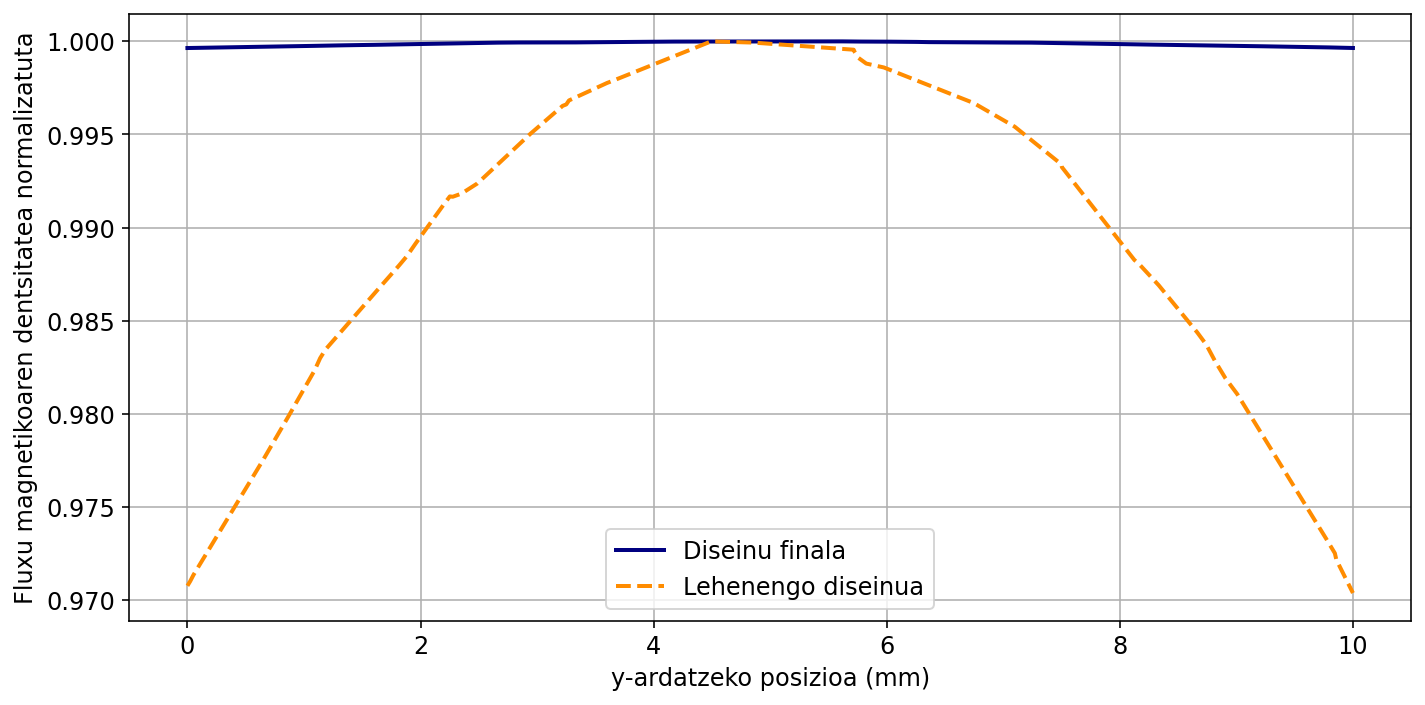
\includegraphics[width=\linewidth]{4 - Diseinua/eremu_magnetikoa_z_normalizatua.png}
    \caption{Iman iraunkorrek $y$-ardatzean sortutako eremu magnetikoaren konparaketa.}
    \label{fig:eremu_magnetikoa_z2}
\end{figure}

Beraz, eremu magnetikoaren balio hori finkatuz eta Wien baldintza erabiliz, eremu elektrikoaren balioa lortu daiteke, eta potentzialak zehaztuz, \textit{Rogowski}-ren profilen eragina ikus daiteke (\ref{fig:eremu_gainezarmena_2}. irudia): eremuen arteko gainezarmena erabatekoa da, baita sarrera eta irteerako zonaldeetan ere.\\

\begin{figure}[h]
    \centering
    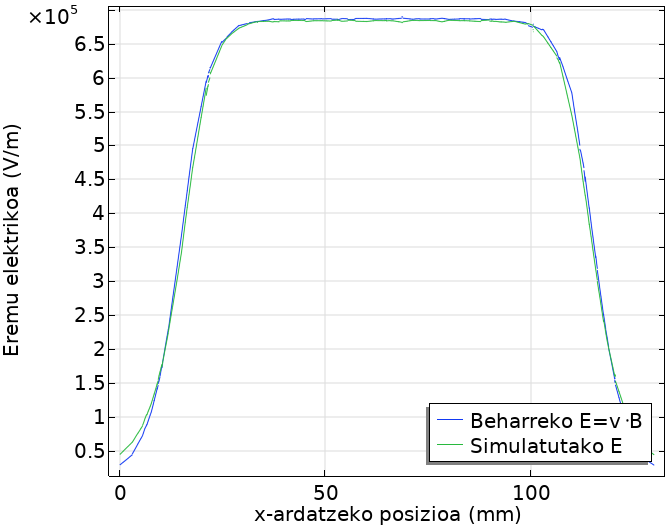
\includegraphics[width=0.6\linewidth]{4 - Diseinua/eremu_gainezarmena_2.png}
    \caption{Eremu elektriko eta magnetikoen gainezarmena ($E_f=B\cdot v_f$) x-ardatzean, \textit{Rogowski}-ren profilak erabiliz.}
    \label{fig:eremu_gainezarmena_2}
\end{figure}
\subsection{Sistema osoaren simulazioak}
Azken diseinuaren fidagarritasuna egiaztatzeko, dispositibo osoa erauzte\hyp{}sistemarekin batera inplementatu da (\ref{fig:sistema_finala_11}. irudia), eta espezie desberdinak aukeratzeko gaitasuna baloratu da. Horretarako, uztarriarekin eremu magnetikoaren balioa aldatu denez ($B'=\num{287}\;mT$), \ref{tab:eremue_balio}. taulan lortutakoa ez da baliagarria, eta elektrodoentzako tentsio berriak kalkulatu behar dira (\ref{tab:eremue_balio_1}. taula).

\begin{table}[h]
    \centering
    \caption{Wien baldintza betetzeko eremu elektrikoak eta potentzialak ($d_e=10\;mm$).}
    \begin{tabular}{cccc}
        \toprule
        \rowcolor{gray!20}
        & $\mathbf{E_{kalkulu}}$ (kV/m) & $\mathbf{V_{\pm}}$ (V)&$\mathbf{E_{simulazio}}$ (kV/m)\\
        \midrule
        $\mathbf{H^+}$ \textbf{aukeratzeko} & $\num{688.11}$ & 3440 & $\num{690.65}$\\
        $\mathbf{H_2^+}$ \textbf{aukeratzeko} & $\num{486.47}$  & 2432 & $\num{486.46}$\\
        $\mathbf{H_3^+}$ \textbf{aukeratzeko} & $\num{397.21}$ & 1986 & $\num{398.88}$\\
        \bottomrule
    \end{tabular}
    \label{tab:eremue_balio_1}
\end{table}

\begin{figure}[h]
    \centering
    \begin{subfigure}[b]{0.52\textwidth}
        \centering
        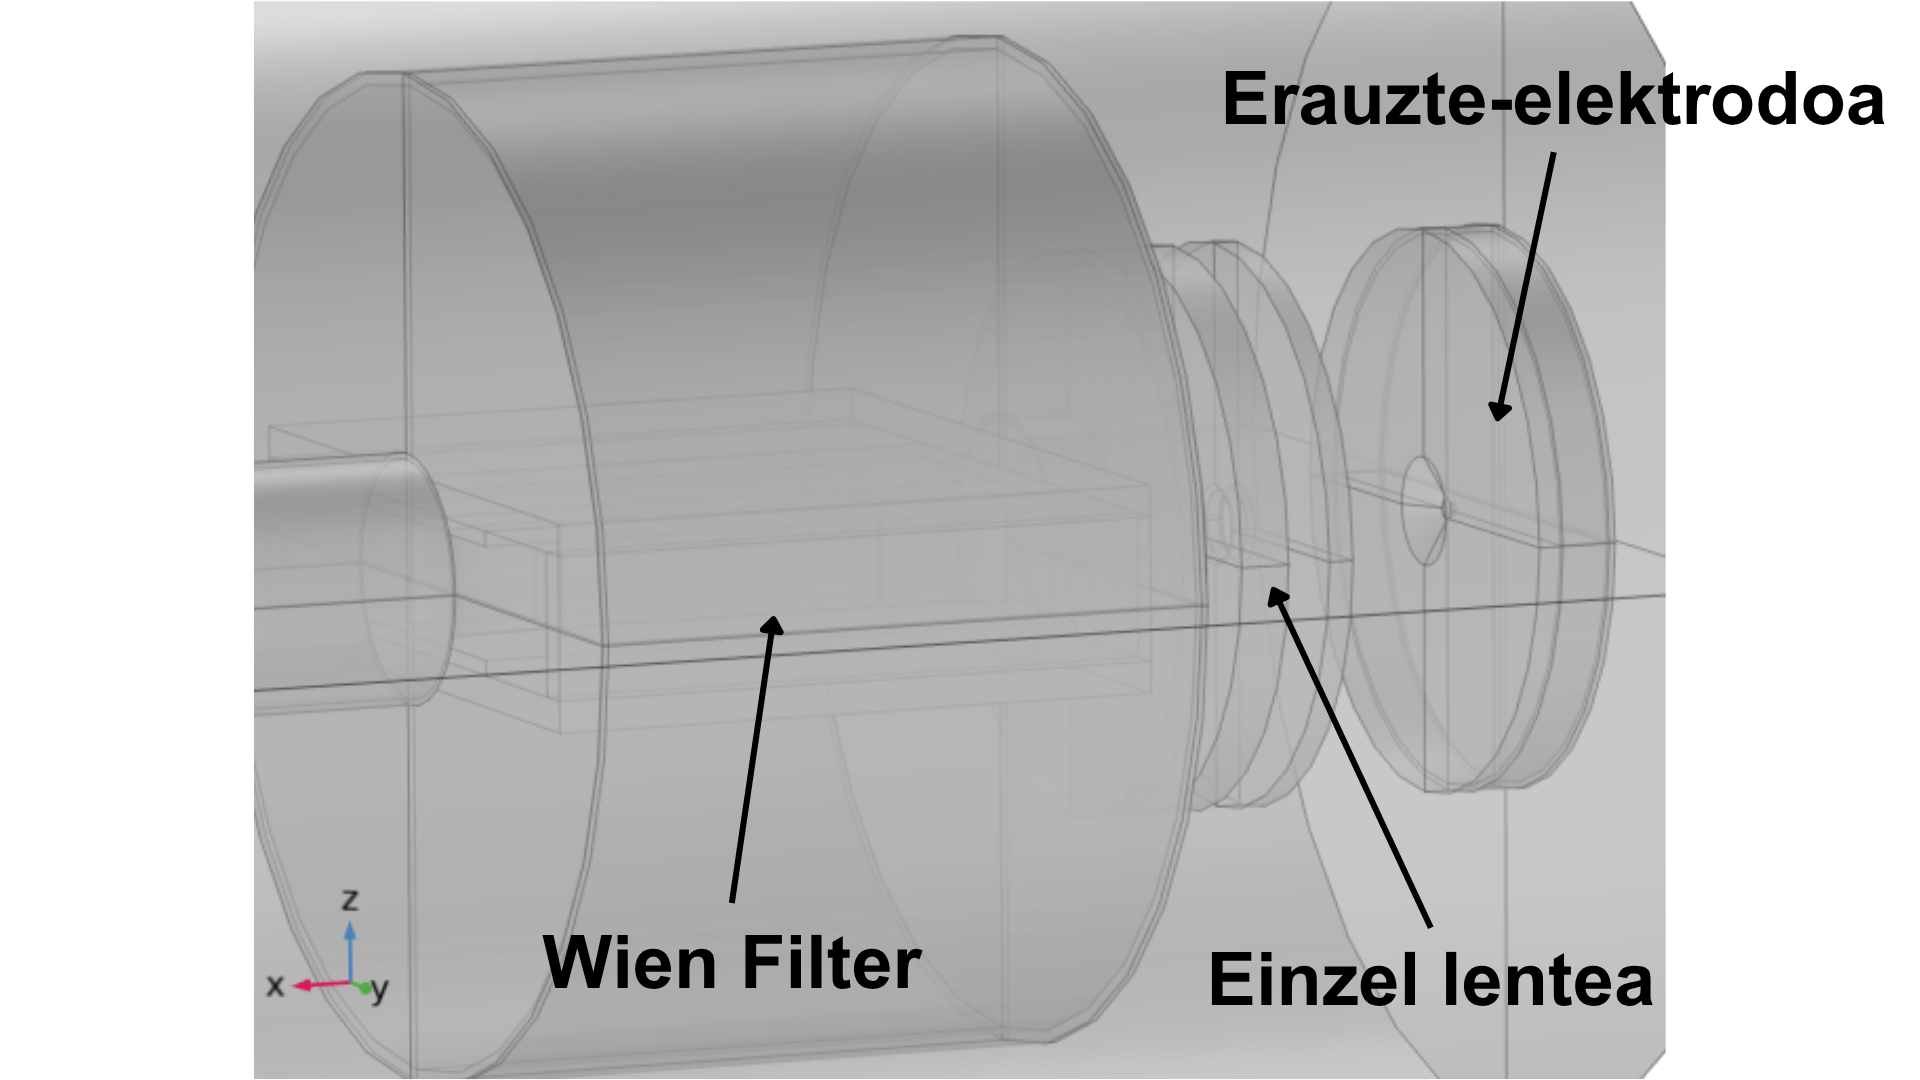
\includegraphics[width=\linewidth]{4 - Diseinua/sistema_osoa_finala.png}
        \caption{Geometria finala 3D-n.}
        \label{fig:sistema_finala_osoa}
    \end{subfigure}
    \hspace{0.02\textwidth}
    \begin{subfigure}[b]{0.4\textwidth}
        \centering
        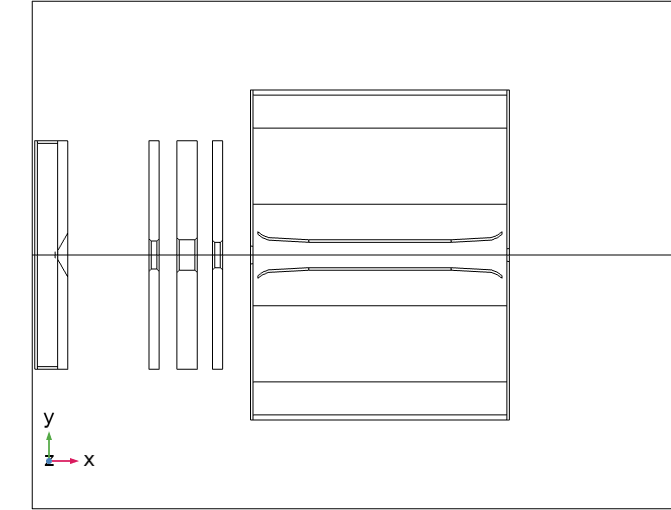
\includegraphics[width=\linewidth]{4 - Diseinua/sistema_osoa_finala_xy.png}
        \caption{Geometria $xy$ planoan.}
        \label{fig:sistema_finala_xy}
    \end{subfigure}
    \caption{Sistema osoaren amaierako diseinua COMSOL-en.}
    \label{fig:sistema_finala_11}
\end{figure}

\begin{figure}[h]
    \centering
    \begin{subfigure}[b]{0.3\textwidth}
        \centering
        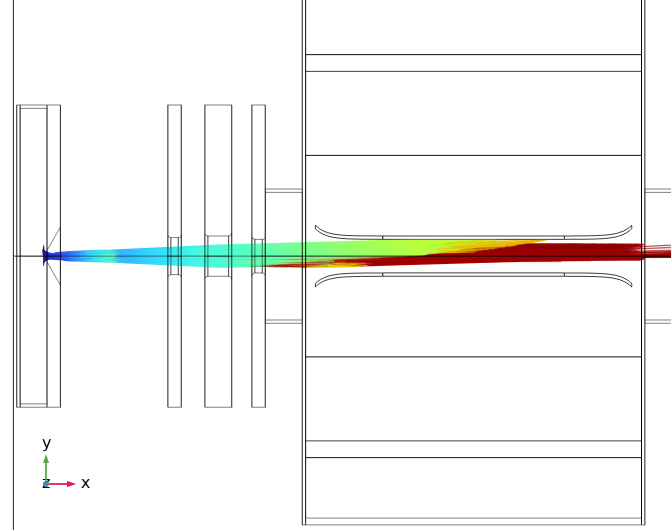
\includegraphics[width=\linewidth]{4 - Diseinua/h+_sistema_osoa.png}
        \caption{\colorbox{red}{$\mathbf{H_{ }^+}$} aukeratuz.}
        \label{fig:sistema_finala_osoa}
    \end{subfigure}
    \hspace{0.01\textwidth}
    \begin{subfigure}[b]{0.3\textwidth}
        \centering
        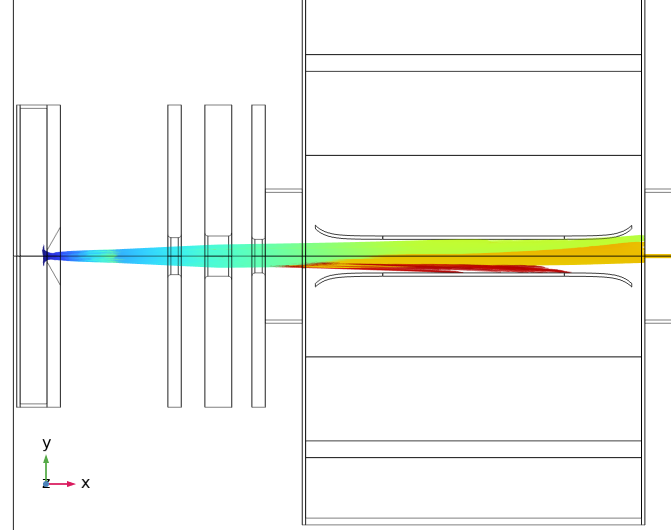
\includegraphics[width=\linewidth]{4 - Diseinua/h2+_sistema_osoa.png}
        \caption{\colorbox{yellow}{$\mathbf{H_2^+}$} aukeratuz.}
        \label{fig:sistema_finala_xy}
    \end{subfigure}
    \hspace{0.01\textwidth}
    \begin{subfigure}[b]{0.3\textwidth}
        \centering
        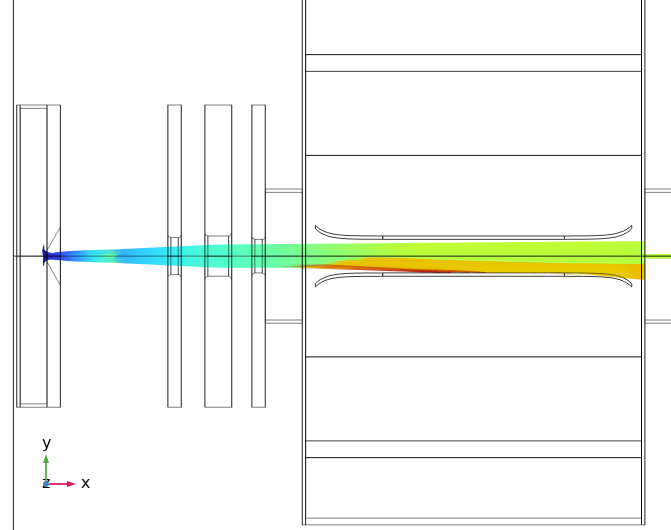
\includegraphics[width=\linewidth]{4 - Diseinua/h3+_sistema_osoa.png}
        \caption{\colorbox{lime}{$\mathbf{H_3^+}$} aukeratuz.}
        \label{fig:sistema_finala_xy}
    \end{subfigure}
    \caption{Partikulen ibilbideak \ref{tab:eremue_balio_1}. taulako tentsioen balioetarako.}
    \label{fig:iragazketa}
\end{figure}

Iragazkiko elektrodoetan tentsio horiek aplikatuz gero, espezie desberdinak aukeratzea posiblea dela frogatu da, beste espezieak guztiz iragaziz (\ref{fig:iragazketa}. irudia). Hala ere, potentzialentzat lortutako balioak adierazpen teorikoetan oinarrituta daude, eta posiblea da espezie bakoitzaren korrontea maximizatzeko balio zehatzak ez izatea. Hori dela eta, komenigarria da iragazkia eraiki ondoren potentzialen ekorketak egitea, izpiaren korronteak neurtuz eta balio maximoei erreparatuz.\\

Bestalde, nahiz eta ertz-efektuak leundu diren, eremu magnetikoa ez da guztiz uniformea $y$-ardatzan, eta beraz, Wien baldintza puntuz puntu desberdina da. Hori dela eta, nahiz eta iragazkira sartzen diren partikulek abiadura berdina izan, ertzetako partikulek indarrak jasaten jarraitzen dute, izpiaren formari eta emitantziari eraginez \cite{Yasuda:2019rzc}.

\begin{figure}[h]
    \centering
    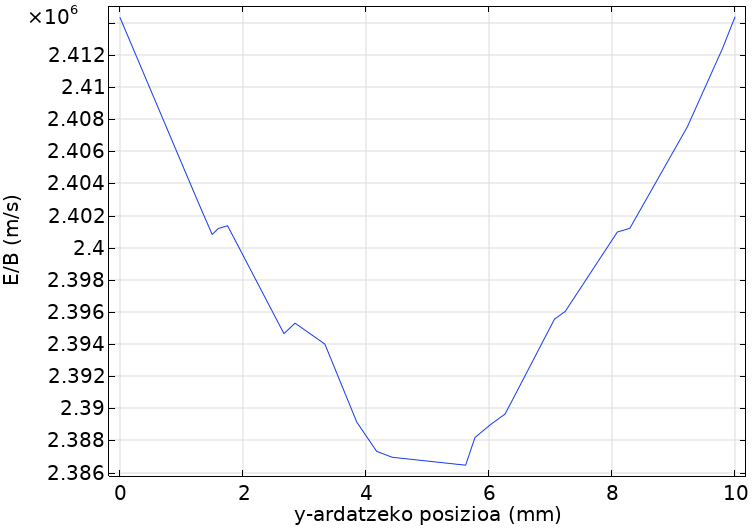
\includegraphics[width=0.5\linewidth]{4 - Diseinua/wien_baldintza.png}
    \caption{Wien baldintzak zehaztutako abiadura $y$-ardatzan, protoiak aukeratuz.}
    \label{fig:wien_baldintza}
\end{figure}

Izpiaren ezkerraldeko partikulek Wien baldintza baino abiadura txikiagoa dutenez, indar elektrikoa jasango dute $+y$ norabidean, eta erdian baldintza ondo betetzen dutenez, bertan pilatuko dira. Modu berean, eskuineko partikulek indar elektrikoa jasango dute $+y$ norabidean, baina norabide horretan eremu magnetikoa txikitzen jarraitzen denez, gehiago desbideratuko dira.

\begin{figure}[h]
    \centering
    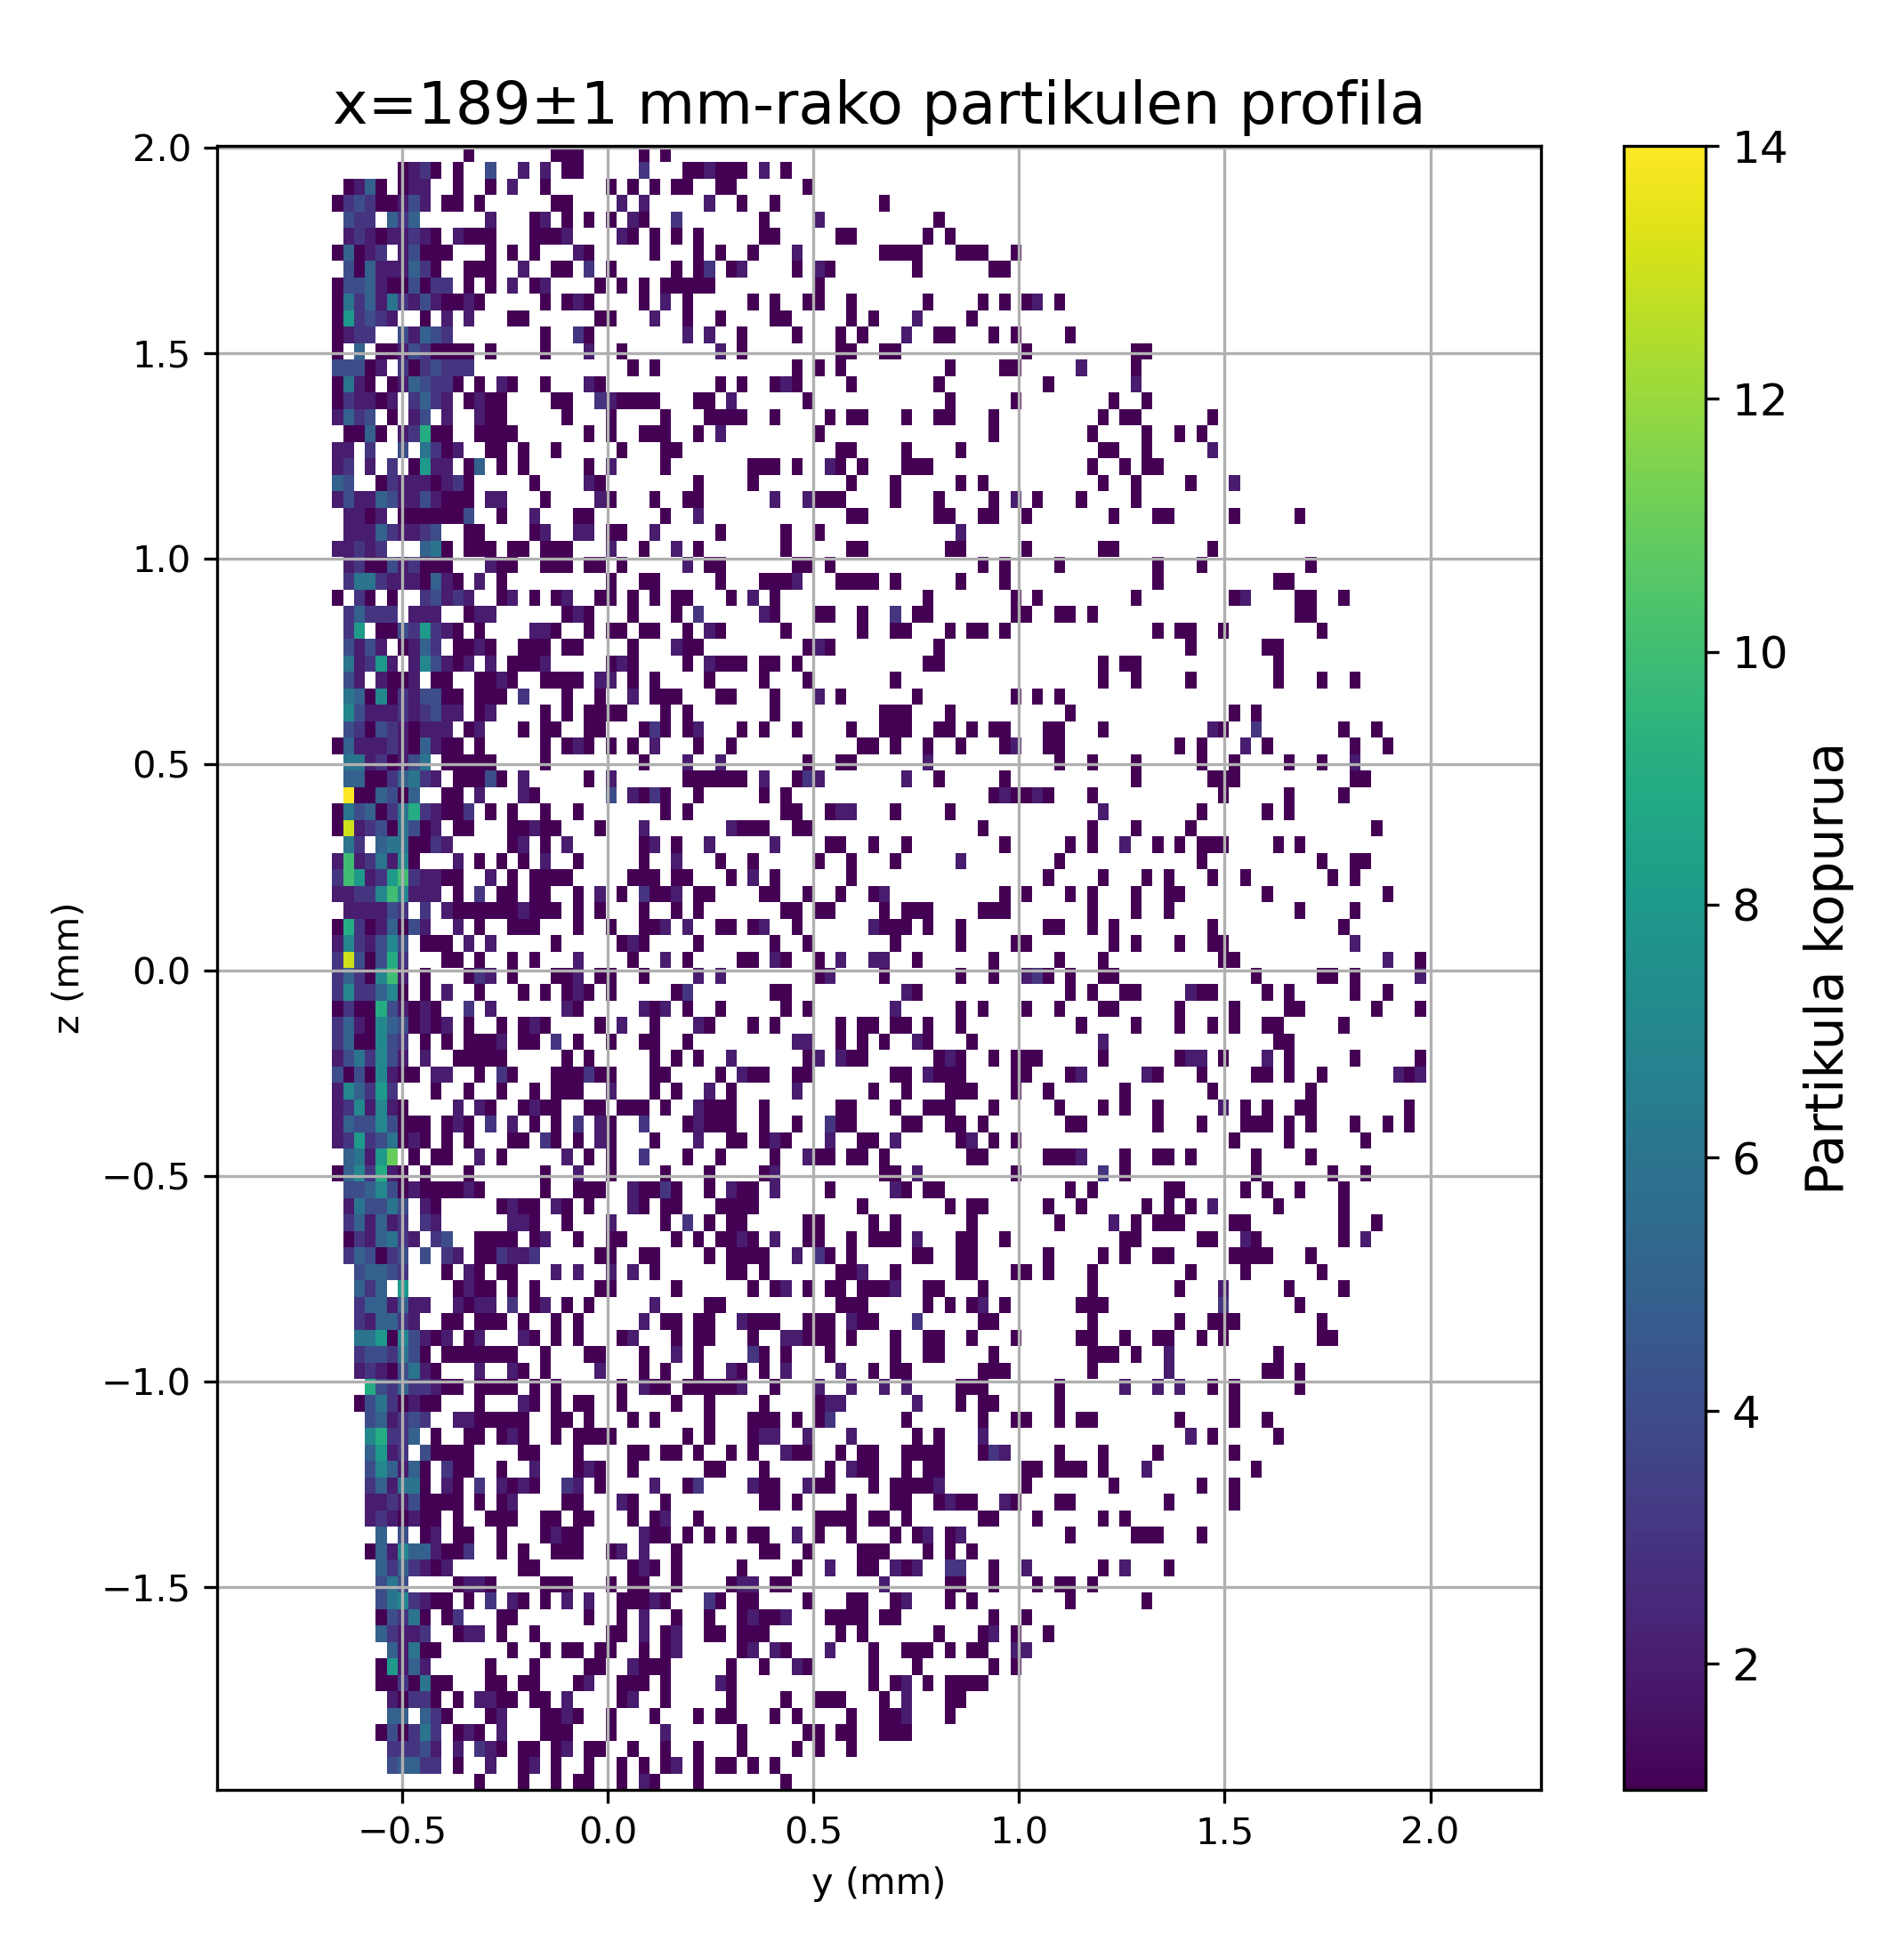
\includegraphics[width=0.4\linewidth]{4 - Diseinua/wien_final_profile.png}
    \caption{Izpiaren profila iragazkiaren amaieran ($x=189\;mm$), protoiak aukeratuz.}
    \label{fig:wien_profile}
\end{figure}

Horrela, amaierako izpiak $D$ itxura du, partikula gehienak bertikalki pilatzen direlarik. Ondorioz, iman iraunkorreko iragazkietan ohikoa da zirrikitu moduko irteerak erabiltzea \cite{zhang_new_2004}. Hala ere, nahiz eta horrek izpiaren biraketa simetria apurtu, LEBT-eko solenoideen fokatzeari esker aurrerago berreskuratuko da. \\

Protoiak aukeratuz ($V_\pm \approx 3450\;V$) eta $r_{out}=\num{0.5}\;mm$ erradioko irteera zirkularra zehaztuz, adibidez, iragazkitik 459 partikula ateratzen dira; hau da, hasieran sortutakoen $\%\num{3.2}$-a. Bestalde, LEBT-aren sarreran lortutako izpia propagazio ardatzan zentratutako elipsoide bertikala da, eta kalkulatutako emitantziak \ref{tab:final_emittances}. taulan ikus daitezke, izpia dibergentea izanik (\ref{fig:final_emittances}).

\begin{figure}[h]
    \centering
    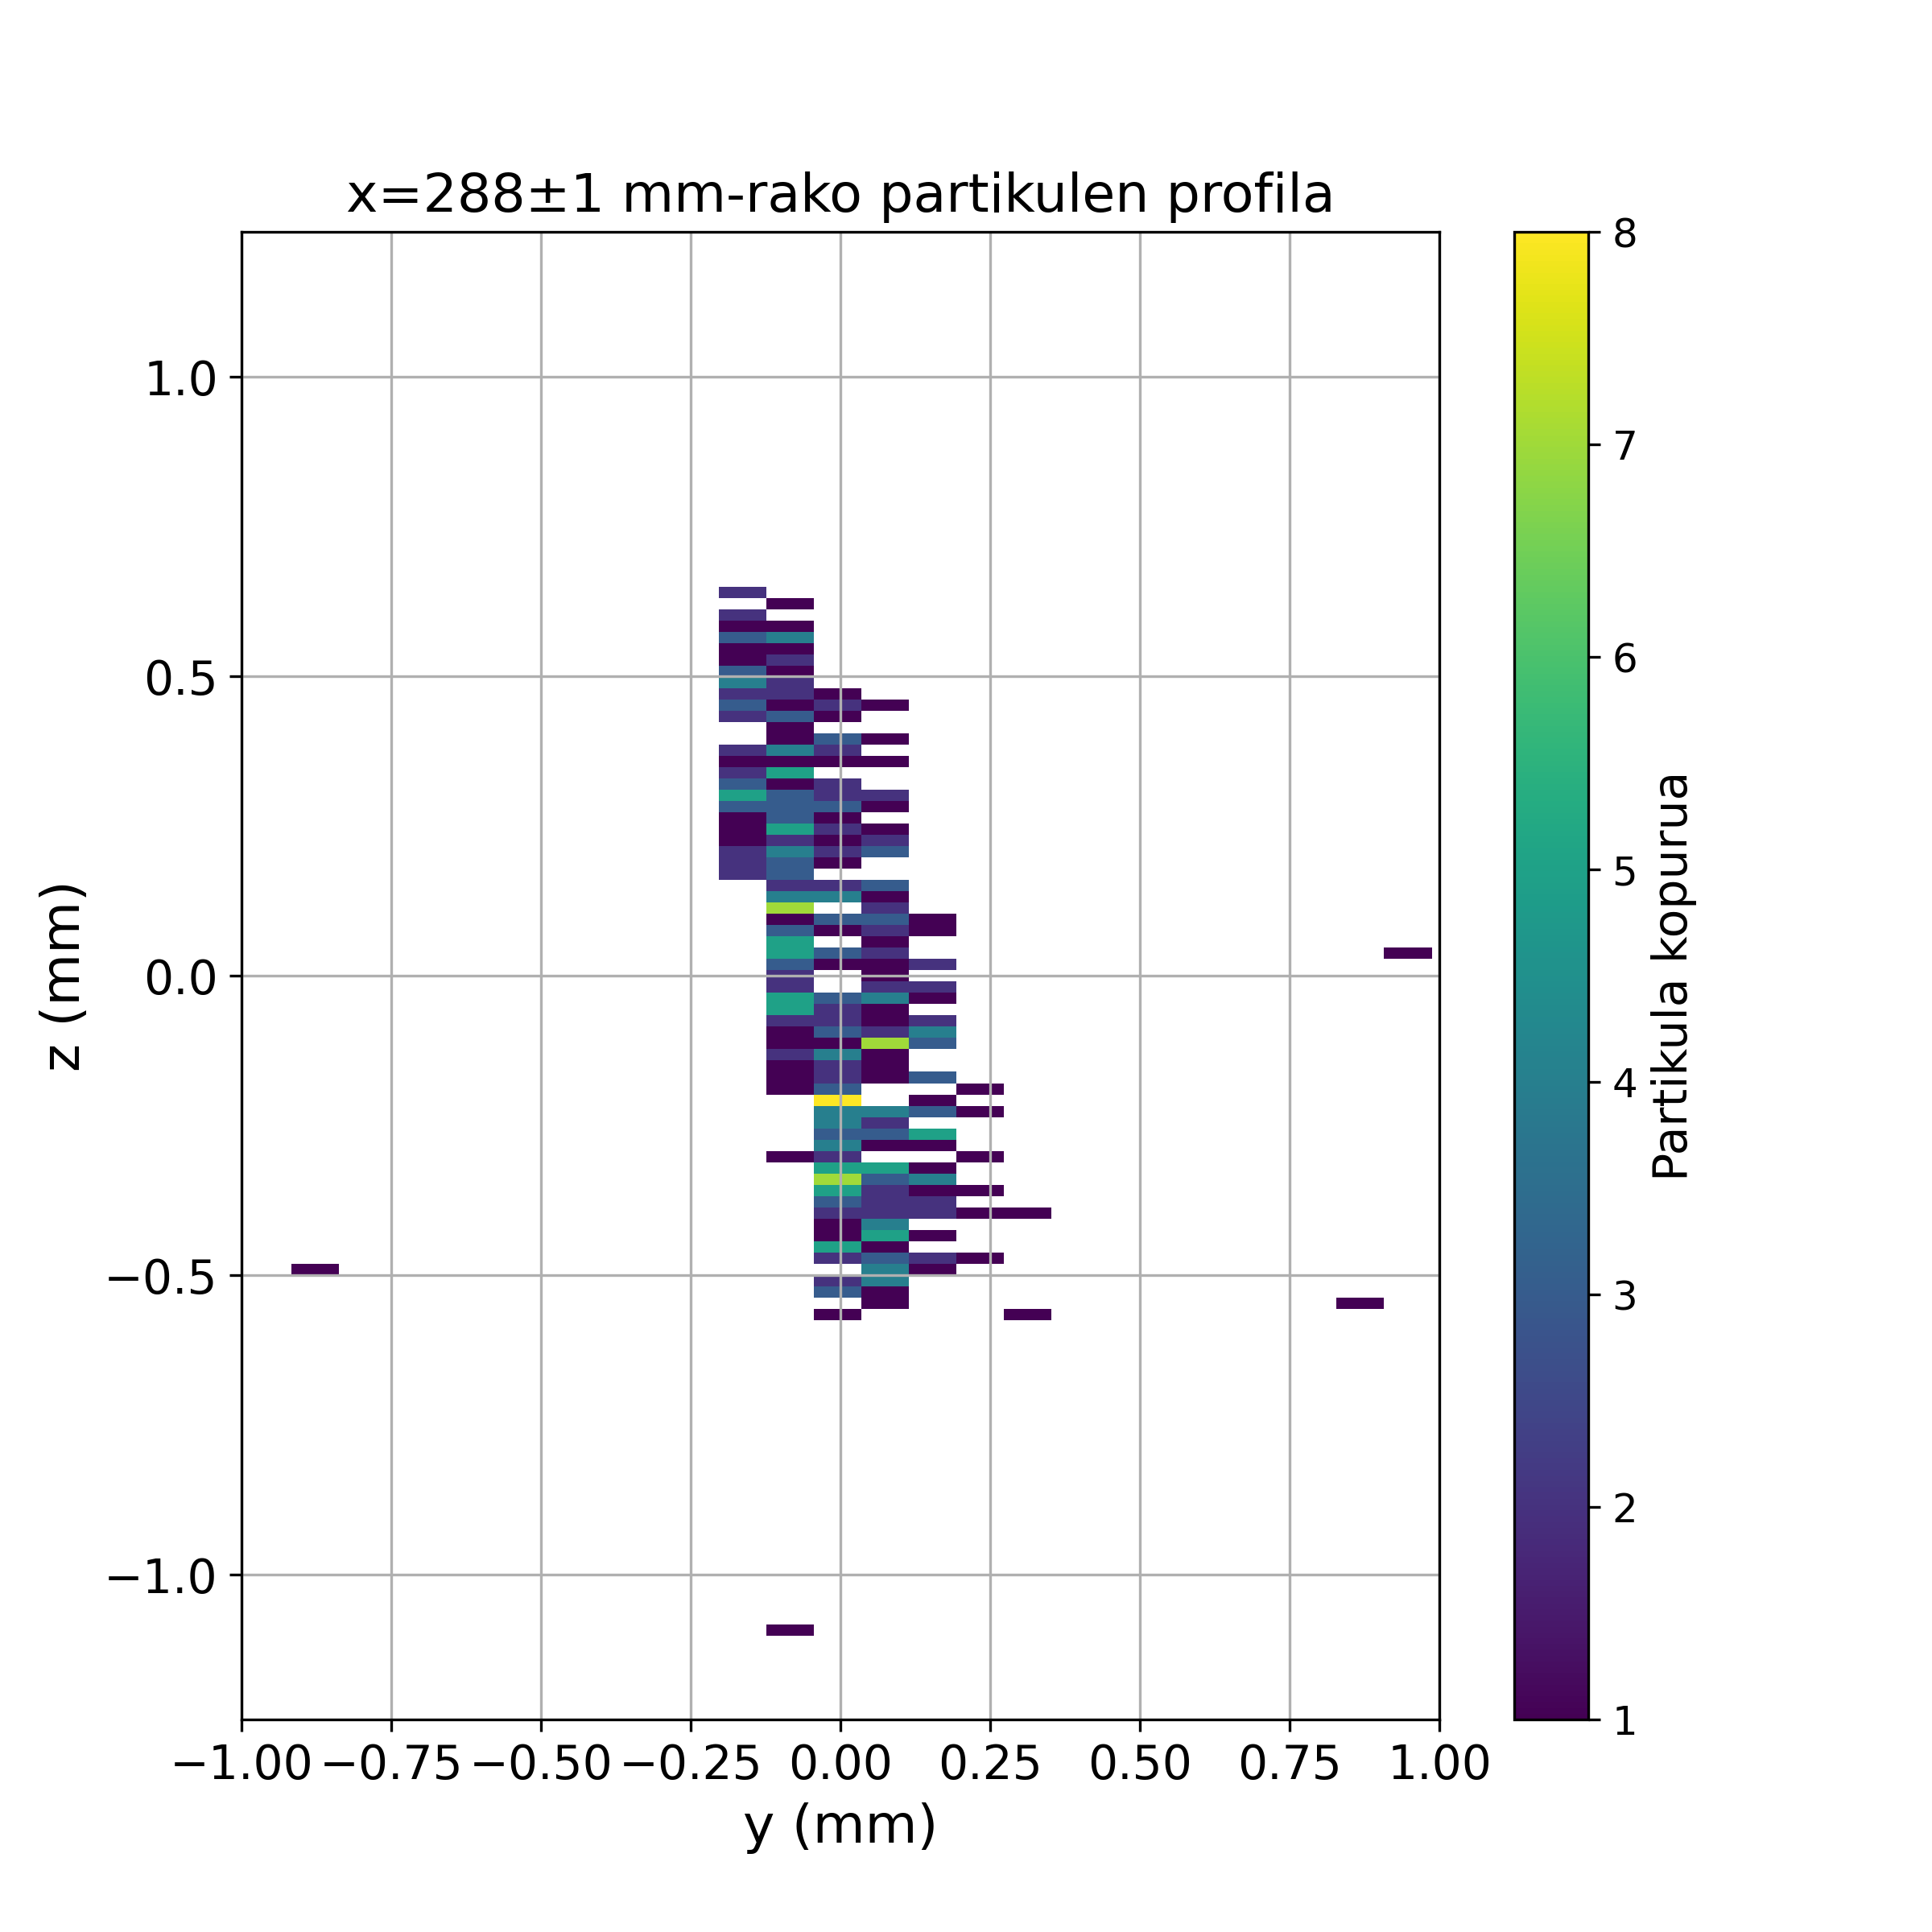
\includegraphics[width=0.38\linewidth]{4 - Diseinua/lebt_profile.png}
    \caption{Izpiaren profila LEBT-aren sarreran ($x=288\;mm$).}
    \label{fig:kolimazio_profil}
\end{figure}

\begin{table}[h]
    \centering
    \caption{Emitantzien ($mm\;mrad$) konparaketa.}
    \begin{tabular}{ccc}
        \rowcolor{gray!20}
        \toprule
         & \textbf{$\epsilon_{yy',\mathrm{rms}}$} & \textbf{ $\epsilon_{zz',\mathrm{rms}}$}\\
        \specialrule{0.5pt}{0pt}{5pt} 
        Einzel lentearen irteeran & $\num{2.508}$ & $\num{2.651}$ \\
        LEBT-aren sarreran & $\num{1.673}$ & $\num{0.491}$\\
        \bottomrule
    \end{tabular}
    \label{tab:final_emittances}
\end{table}

\begin{figure}[h]
    \centering
    \begin{subfigure}[b]{0.38\textwidth}
        \centering
        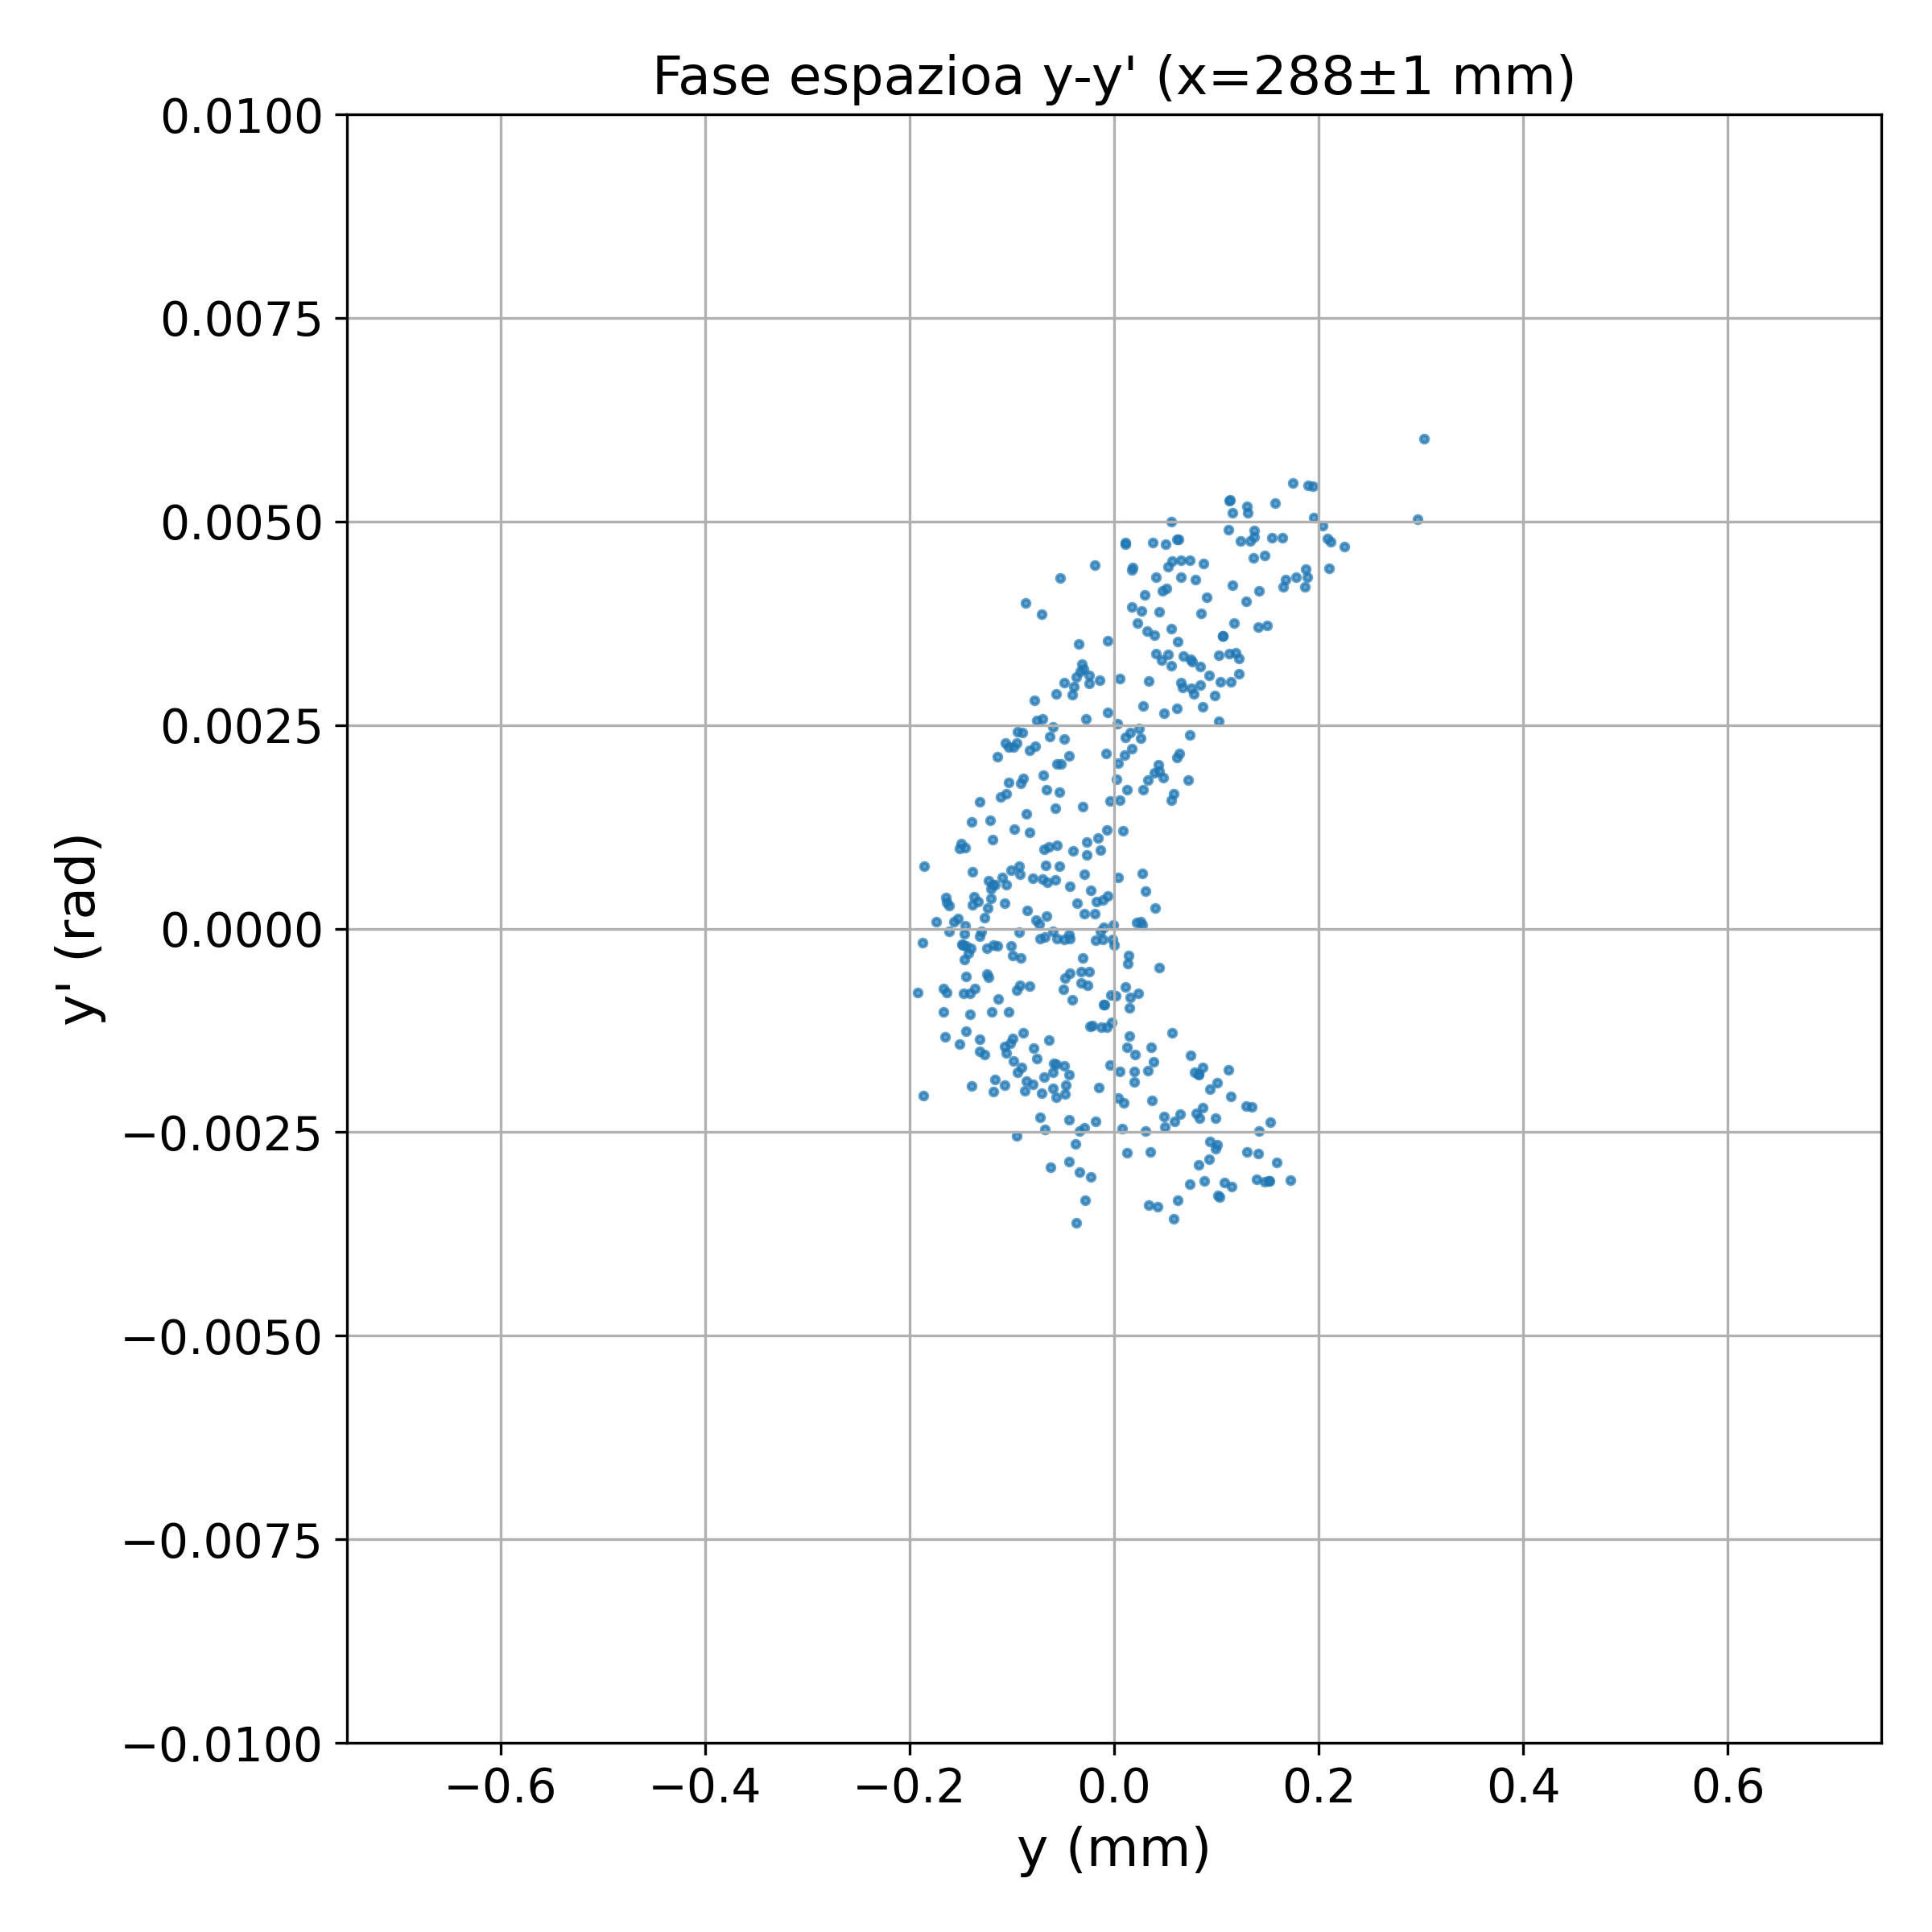
\includegraphics[width=\linewidth]{4 - Diseinua/lebt_emitantzia_y.png}
        \caption{$yy'$ planoan.}
        \label{fig:final_emitantzia_y}
    \end{subfigure}
    \hspace{0.02\textwidth}
    \begin{subfigure}[b]{0.38\textwidth}
        \centering
        \includegraphics[width=\linewidth]{4 - Diseinua/lebt_emitantzia_z.png}
        \caption{$zz'$ planoan.}
        \label{fig:final_emitantzia_z}
    \end{subfigure}
    \caption{LEBT-aren sarreran ($x=288\;mm$) lortutako aztarna-espazioak.}
    \label{fig:final_emittances}
\end{figure}



\newpage
\section{Ondorioak eta etorkizuna}
Lan honetan Linac-7 azeleragailurako \textit{Wien Filter} baten lehen diseinua eta simulazioak garatu dira. Horretarako, hauek izan dira landutako atalak, eta baita horietan lortutako ondorioak.\\

Lehenik eta behin, Mikel Elorzak garatutako hidrogeno plasmaren modelizazioa landu da, izpiaren karakterizazio zehatza lortzeko eta baita plasmaren parametro operazionalekiko portaera hobeto ulertzeko. Espezie ionikoen frakzioak lortuz, \textbf{sistemaren portaera errealista lortu} da, simulazioen emaitzak ahalik eta erabilgarrienak izateko. Bestalde, \textbf{ioi-izpien portaera ondo ulertzea} lortu da, propietateak definituz eta horiek manipulatzeko beharreko lente elektrostatikoak teorikoki garatuz.  \\

Ondoren, COMSOL Multiphysics softwarea aurkeztu da, iragazkiaren diseinurako erabilitako tresna. Proiektuko aurreko simulazioetan SIMION softwarea erabiltzen zenez, bi programak konparatu dira, eta COMSOL-en emaitzak SIMION-en lortutakoekin balidatu dira erauzketa sistemarako. Horrela, proiektuaren etorkizuneko lanetan \textbf{COMSOL erabili daitekeela ziurtatu} da, eta baita erauzketa sistemaren eta iragazkiaren artxiboak eskuragarri utzi dira.\\

Iragazkiaren diseinuan, oinarri teorikoan garatutako elektrodo paraleloek eta aurrez-aurreko iman iraunkorrek sortutako mugapenak azaleratu dira: ertz-efektuak. Orduan, horiek leuntzeko, \textit{Rogowski}-ren profilak eta burdin gozozko uztarria eraginkorrak direla erakutsi da, eta horiek erabiliz \textbf{hidrogeno espezie desberdinak iragaztea lortu} da amaieran.\\

Hori guztia kontuan hartuta, hasieran planteatutako helburuak bete dira, eta gainera, lanak hainbat erronka irekita uzten ditu, etorkizunean bai graduko bai graduondoko ikerketetarako aukera emanez:\\

\begin{enumerate}
    \item Irteerako irekiduraren hautaketa zehaztu behar da. Iman iraunkorren sistema mantentzen bada, horiek sortutako eremua guztiz uniformea ez denez, zirrikitua erabili daiteke, sistemaren simetria zirkularra hautsiz, baina intentsitatea maximizatuz. Bestalde, eremu magnetiko uniformeagoa sortzeko, elektroimanak erabili daitezke ere, irekiera zirkularra mantenduz.
    \item Iragazkiaren diseinu mekaniko zehatza egin daiteke, gaur egungo sisteman akoplatzeko. Gainera, azeleragailuan hutsa beharrezkoa denez, dispositiboaren huts sistema landu behar da.
    \item Materialen iraunkortasuna ere aztertu daiteke: espezieak desbideratzean dispositiboaren elementuekin talka egiten dutenez, materialek higadura jasango dute, eta erabileran eragin dezake.
    \item Prototipoa eraiki eta esperimentalki testatu daiteke simulazioen fidagarritasuna egiaztatzeko, eta diseinuan aukeratutako balioak doitzeko ere: imanen arteko distantzia, elektrodoen arteko distantzia, potentzialen aukeraketa neurtutako intentsitatearen arabera...
\end{enumerate}



\section{Garapen Iraunkorrerako Helburuak}
Lan hau Nazio Batuen Erakundeko (NBE) Garapen Iraunkorrerako 2030 Agendako hainbat helburuekin lerrokatzen da:\\

\begin{itemize}
    \item \textbf{3. GIH: Osasuna eta ongizatea.} Linac-7 proiektuaren helburu nagusia PET (\textit{Positron Emission Tomography}) diagnostikorako erabiltzen diren isotopoak lokalki ekoiztea da, aktibitate handiko eta erdibizitza luzeko isotopo garesti eta arriskutsuak saihesteko. Lan honen bidez, azeleragailu trinko eta merkeen garapena bultzatzen da, gaixoen tratamendu azkarragoa eta seguruagoa eskaintzeko.
    \item \textbf{4. GIH: Kalitatezko hezkuntza.} Lan honek ezagutza teknikoa euskaraz garatzea eta zabaltzea ere du helburu. Arlo teknikoetan, euskararen presentzia mugatua denez, ezinbestekoa da maila altuko baliabideak euskaraz sortzea, hezkuntza-sistemaren kalitatea hobetzeko.
    \item \textbf{9. GIH: Industria, berrikuntza eta azpiegitura.} Lan honetan diseinatzen den \textit{Wien filter}-a azeleragailu linealen funtsezko etapa da, eta diseinu orokorra izanik, beste azeleragailu linealetan ere erabil daiteke. Gainera, Linac-7 proiektuan Euskal Herriko enpresekin lan egiten denez ere (Tekniker, Egile), tokiko industria-ehuna sendotzea du helburu.
\end{itemize}
\newpage
\printbibliography

\newpage
\appendix
\section{Eranskina: Garraio-matrizeen garapena}
\label{ap:matrizeak}
\paragraph{Eremu elektrostatiko uniformea}\leavevmode\\

$V_1$ eta $V_2$ potentzialeko planoen artean $\vec{E}=E\cdot \hat{z}$ eremu-elektriko konstante bat sortzen da (\ref{fig:euniforme}. irudia). Partikula baten energia zinetikoa $V_i$ potentzialeko edozein puntutan $qV_i$ bada, higidura-ekuazio diferentzialak eta hasierako baldintzak,

\begin{equation}
   \begin{aligned}
    m\ddot{r}&=0 \qquad m\ddot{z}=qE\\
    z_1 = r_1 = 0 \qquad \dot{r}_1&=v_1sin\,\alpha_1 \qquad v_1 = \sqrt{2q\frac{V_1}{m}}
    \end{aligned} 
\end{equation}
\\ 
zuzenean integratu daitezke,

\begin{equation}
    \begin{aligned}
        \dot{z}=\frac{qE}{m}t+v_1 cos\, \alpha_1 \xRightarrow{} z&=\frac{qE}{2m}t^2+v_1 cos\, \alpha_1 \cdot t\\
        \dot{r}=\dot{r}_1=v_1sin\, \alpha_1 \xRightarrow{} \ r&= v_1 sin\,\alpha_1 \cdot t
    \end{aligned}
\end{equation}
\\
eta t askatuz eta ordezkatuz, partikularen ibilbidea lortu,

\begin{equation}
    \frac{qE}{2mv_1}t^2+ cos\, \alpha_1 \cdot t - \frac{z}{v_1}=0 \xRightarrow{} r= \frac{2V_1}{E}sin\, \alpha_1 \cdot(\sqrt{\frac{E}{V_1}z+cos^2\alpha_1}-cos\,\alpha_1)
\end{equation}
\\
Beraz, garraio-matrizea lortzeko, $V_2$ potentzialeko planoko posizioa eta malda lortu behar dira. Eremu elektrikoa $E=\frac{V_2 - V_1}{L}$ modura hurbilduz,\\
\begin{equation}
    \begin{aligned}
         r_2 &= r(z=L) = \frac{2L sin\, \alpha_1}{\frac{V_2}{V_1}-1}\cdot(\sqrt{\frac{V_2}{V_1}-sin^2\alpha_1}-cos\, \alpha_1)\\
         r_2'&=\frac{dr}{dz}|_{z=L}=sin\, \alpha_1 \cdot(\frac{V_2}{V_1}-sin^2\alpha_1)^{-\frac{1}{2}}
    \end{aligned}
    \label{eq:eremuuniforme}
\end{equation}


\begin{figure}[h]
    \centering
    \includegraphics[width=0.9\linewidth]{2 - Oinarri teorikoa/eremuuniforme.png}
    \caption{Ioi baten azelerazioaren eskema eremu elektriko uniforme batean \cite{liebl_applied_2008}.}
    \vspace{-15pt}
    \label{fig:euniforme}
\end{figure}

Azkenik, \eqref{eq:eremuuniforme} adierazpenean hurbilpen paraxiala erabiliz ($\alpha_1\ll1$), $sin\, \alpha_1 \approx r_1'$ eta $cos\, \alpha_1 \approx 1$ moduan hurbilduz, eta bigarren ordenako elementuak arbuiatuz,

\begin{equation}
    \begin{aligned}
        r_2 &\approx \frac{2Lr_1'}{\frac{V_2}{V_1}-1}(\sqrt{\frac{V_2}{V_1}-1}) =\frac{2L}{\sqrt{\frac{V_2}{V_1}}+1} r_1'\\
        r_2' &\approx \sqrt{\frac{V_1}{V_2}}r_1'
    \end{aligned}
\end{equation}\\

Horrela, garraio-matrizea lortu dezakegu, $r\neq 0$ denean $\tilde{r_2}=r_1+r_2$ eginez,

\begin{equation}
\boxed{
    R_U = \begin{pmatrix}
            1 & \frac{2L}{\sqrt{V_2/V_1}+1}\\
            0 & \sqrt{\frac{V_1}{V_2}}
    \end{pmatrix}
}
\end{equation}

\paragraph{Irekiera zilindrikoko elektrodoak}\leavevmode\\

Praktikan, ordea, ioiek ez dituzte potentzial planoak zeharkatzen, baizik eta potentzial horiek dituzten elektrodoetako irekieretatik igarotzen dira. Irekiera horien inguruan, gainazal-ekipotentzialak kurbatzen dira, eremu-elektrikoaren osagai erradialak sartuz, $E_r$. Hori dela eta, irekierek lente moduan jokatzen dute.

\begin{figure}[h]
    \centering
    \includegraphics[width=0.8\linewidth]{2 - Oinarri teorikoa/aperture_lens.png}
    \caption{Eremu elektrikoaren gainazal-ekipotentzialen kurbatzea irekieretan.}
    \label{fig:enter-label}
\end{figure}

Eremu elektrikoaren fluxu-lerroen kontserbaziotik hurrengoa lortu daiteke, karga\hyp{}espaziorik ez badago,

\begin{equation}
    r^2 \pi E_1 + 2 r \pi \int_{-a}^{+b} E_r dz=r^2 \pi E_2 \quad \Longrightarrow \quad r(E_1-E_2)+2\int_{-a}^{+b} E_r dz=0
    \label{kontserbazio}
\end{equation}
\\
non −a eta +b mugak irekieraren inguruko eremu elektriko erradiala esanguratsua den z ardatzeko tartea adierazten duten. Ezkerretik eskuinera igarotzen den ioiek jasandako momentu erradiala, $v_z =\frac{dz}{dt}$ izanik,

\begin{equation}
    \begin{aligned}
    mv_r&= -\int qE_rdt
    \end{aligned}
    \quad \Longrightarrow \quad
    mv_r = -\frac{q}{v_z}\int_{-a}^b E_r dz
\end{equation}\\

Ibilbidea paraxiala izanik, $v_x$ konstantetzat hartu daiteke, eta \eqref{kontserbazio} ordezkatuz, hurrengo aldaketa erradiala lortzen da,

\begin{equation}
    mv_r=\frac{qr}{2v_z}(E_1-E_2) \quad \Longrightarrow \quad \Delta r' = \frac{v_r}{v_z}=\frac{q(E_1-E_2)}{2mv_z^2}r
\end{equation}\\

Orduan, $r_2=r_1$ eta $r_2'=r_1'+\Delta r'$ direla kontuan hartuz, garraio-matrizea,\\

\begin{equation}
\boxed{
    R_A = \begin{pmatrix}
            1 & 0\\
            \frac{q(E_1-E_2)}{2mv_z^2} & 1
    \end{pmatrix}
}
\end{equation}\\

\end{document}
